%!TEX TS-program = xelatex
%!TEX encoding = UTF-8 Unicode

\documentclass[dsingle]{Dissertate}

\begin{document}

% the front matter
%!TEX root = ../dissertation.tex
% Some details about the dissertation.
\title{Development and Application of a Computational Platform for Complex Molecular Design}
\author{Jaime Rodríguez-Guerra Pedregal}

%If you have one advisor
\advisor{Prof. Dr. Jean-Didier Maréchal}
\tutor{Prof. Dr. Jordi Joan Cairó Badillo}
\committeeInternalOne{Person Inside One}
\committeeInternalTwo{Person Inside Two}

%If you are coadvised
\coadvisorOne{Delightful Researcher}
\coadvisorTwo{Equally D. Researcher}
\committeeInternal{Person Inside}

% Everyone has an External committee member
\committeeExternal{Person Outside}

% ... about the degree.
\degree{Doctor of Biotechnology}
\field{Biotechnology}
\degreeyear{2018}
\degreeterm{Summer}
\degreemonth{July}
\department{Department of Chemistry}

% ... about the candidate's previous degrees.
\pdOneName{B.S.}
\pdOneSchool{Universidad de Salamanca}
\pdOneYear{2013}

\pdTwoName{M.S.}
\pdTwoSchool{Universitat Autònoma de Barcelona}
\pdTwoYear{2014}

\frontmatter
%\listoftodos

\makeatletter
    \if@twoside
        \pagestyle{fancy}
        \fancyhf{}%
        \renewcommand{\headrulewidth}{0pt}%
        \renewcommand{\chaptermark}[1]{\markboth{#1}{}}
        \fancyhf[leh,roh]{\thepage}%

    \fi
\makeatother
\setstretch{\dnormalspacing}

% % include each chapter...
%\setcounter{chapter}{4}  % start chapter numbering at 0
%!TEX root = ../dissertation.tex

\chapter*{Preface}
\addcontentsline{toc}{chapter}{Preface}
\label{chap:preface}

\Lettrine{Scientific} progress is tightly linked to human curiosity, a driving force that has brought us further and further every decade. The same impulses that thrusted imagination into wondering what those lights in the sky are, kept us on Earth trying to figure out how far we can get splitting matter into pieces. A mountain can be reduced to rocks, stones, pebbles, sand, dust and$ \ldots $  where do we stop? That question gave birth to the \textit{atomism} philosophy in Ancient Greece, when the term for the modern word \textit{atom} was coined: \textit{ἄ$\tau$ο$\mu$ο$\nu$ (atomon, indivisible)}. In atomism, all matter is composed of atoms and void. Those philosophical atoms, in all shapes and sizes, could collide with each other or hook together to form clusters resulting in their observable, macroscopic counterparts or \textit{substances}.

\textit{Atomism} was just a philosophical current trying to explain the world without any empirical observations to prove those hypotheses. It can be considered the first atomic model; albeit a useless one. This does not necessarily mean it is a bad model. Models are \textbf{simplifications of reality that can provide explanations and predictions of reproducible observations}. In this case, atomism failed to explain actual phenomena, but did satisfy the philosophical curiosity behind its inception. As a result, one can only assess the quality of a model in terms of its purpose: it will be valid as long as this is fulfilled (see fig. \ref{fig:penicillin}).



\begin{figure}[H]
	\includegraphics[width=\textwidth]{./figures/01/penicillin.jpg}
	\cprotect\caption[Dorothy M. Crowfoot's 1945 Penicillin model]{In the pre-computer era, models were built physically. Here depicted, Dorothy M. Crowfoot's 1945 penicillin model. Reproduced from UK's Science Museum.\cite{uksciencemuseum}}
	\label{fig:penicillin}
\end{figure}


Since the clusters described by atomism do not provide useful predictions on molecules, new models have been described over the past decades, each replacing the previous one to address new conflicting observations: Dalton, Thomson, Rutherford, Bohr$ \ldots $ \  During the past century, we have seen the atom acquiring unthought complexity: nuclei, electrons, protons, neutrons, quarks$ \ldots $  Harnessing this complexity in a new model does not mean that we always use the most sophisticated theories. Sometimes, it is simply overkill and unnecessary. The same way relativistic effects are not considered during the preparation of a cheesecake, quantum effects can be ignored in some types of studies. Other times, they must be considered, though.

The complexity of the underlying theory of a model usually correlates with the mathematical principles behind, so the more complex a model becomes, the harder it is to apply it. Even if the model itself it is not mathematically complex, the accumulated steps to obtain a satisfactory answer can make it costly. Fortunately, the uprising of computation in last decades has greatly eased the resolution of the equations proposed by the advances in theoretical chemistry. In fact, the marriage of modeling and computation is so widespread that when one says ‘modeling’, it is commonly understood as ‘computational modeling’.

% Something personal here

When I first started this Ph. D., I did not know the grounds I was standing on. I was very interested in computers and technology, but I had reduced experience with programming. The fascinating field of molecular modeling, and in particular its structural aspects, gave me something visual to work with and taught how little changes in an algorithm can have radical effects on the modeled structure. The following chapters will tell the story of how I found passion in research.

\todo[inline]{Repasar esto}

\makeatletter
    \if@twoside
        \fancyhf[loh]{\textit{\leftmark}}%
        \fancyhf[reh]{\textit{Chapter \thechapter}}
    \fi
\makeatother

%!TEX root = ../dissertation.tex

\begin{savequote}[0.6\textwidth]
	\itshape I suppose it is tempting, \\
	\itshape if the only tool you have is a hammer, \\
	\itshape to treat everything as if it were a nail.
	\qauthor{---Peter H. Salus}
\end{savequote}

\chapter{Introduction}
\label{chap:01}

\Lettrine{Molecular} modeling and simulation, defined as the use of \textbf{computational methods to describe the behavior of matter at the atomistic or molecular level},\cite{maginn2009} comprises a large array of software designed to solve very different problems in wide areas of molecular biology and theoretical chemistry: characterization of reaction profiles, drug discovery, optimization of catalytical processes$ \ldots $  A good modeler knows which techniques and theories must be applied depending on the task at hand, which is even more difficult if one has to take into account the software diversity. Just choosing where to begin can be a daunting task.

This introductory chapter will provide a brief overview on: (1) the major software categories in molecular modeling, which will be further detailed in \autoref{chap:02}; (2) how they can be used together in integrative approaches; and (3) the difficulties, caveats and pending challenges present in these approaches.

\section{In silico molecular modeling}
% \addcontentsline{toc}{section}{In silico molecular modeling}
\subsection{Overview of molecular modeling tools}
% \addcontentsline{toc}{subsection}{Overview of molecular modeling tools}

After decades of development, the number of readily available computational tools can be overwhelming. Depending on the phenomena studied, different techniques are more appropriate than others. This section only provides an overview on the fields and hills that populate the current landscape. A more detailed description on the available techniques can be found in \autoref{chap:02}.

The most popular task performed in molecular modeling consists of describing the energetics of a system, which can then be used as a proxy for structure optimization, reaction path guessing or studies on dynamic behavior, among others. Depending on the method employed to obtain those energies, the results will resemble the experimental observations with higher or lower accuracy.

Atop the accuracy curve we can find Quantum Mechanics (QM) methods, which are based on quantum chemistry and the equations proposed by Schrödinger in 1925. This family of methods consider electrons explicitly, which allows them to study chemical reactivity with highest precision. However, given the complexity of the calculations involved, even modern hardware cannot deal with more than a few hundred atoms.

The next major family, Molecular Mechanics (MM), discards electronics for the sake of speed and scale. Instead of applying Schrödinger’s theory, it considers molecules as a set of spheres connected by carefully calibrated springs, whose energy is given by Newton’s laws of motion. This results in much simpler calculations which can deal with thousands of atoms almost instantaneously. In fact, their most popular usage is its time-dependent implementation, Molecular Dynamics (MD), which analyzes the evolution of a system over millions of timesteps to obtain an accurate representation on the molecular behavior along a few nanoseconds.

QM and MM can be used simultaneously in the same system using an approach called QM/MM. This hybrid method allows to consider larger structures by splitting the calculations in two regions modeled differently. QM is applied to a reduced part of the system that requires an accurate electronic representation, while the rest of the structure is processed with the simpler MM techniques. Both calculations are then integrated by using hybrid schemes such as IMOMM $ \{ $ $ \} $ , IMOMO $ \{ $ $ \} $  or, most popularly, ONIOM $ \{ $ $ \} $ .

Even though it can be argued that energy calculations are behind every molecular modeling study, not all methods focus on obtaining an accurate value. Sometimes, a distantly close one is enough. For example, protein-ligand docking studies are designed to obtain probable orientations in which a small molecule (ligand) can bind to a bigger one (protein). For this assessment, obtaining an accurate binding energy is not as important as navigating the search space reliably: it is preferred to focus on the fast generation of reasonable candidate poses instead of a locating a true global minimum. To\ do that in an affordable time, accurate energies are normally replaced by scoring functions that return pseudo-energies or even unitless scalars. These functions can be based on simplified molecular mechanics, knowledge-based potentials, shape complementarity or even simple geometric measurements.

Drastic simplifications of energy are not uncommon in molecular modeling, especially if large search spaces must be analyzed efficiently. Normal Mode Analysis (NMA) apply an even simpler ball-and-springs model to obtain the principal vibration frequencies of a molecular structure. Under this approach, collective motions can be assessed in minutes without resorting to long molecular dynamics, which can take days or weeks to finish.

Vast search spaces are not limited to macromolecules with large number of atoms. Every variable considered during an analysis generates an additional dimension in the search space. Any slight change in the topology of the molecule can incur in more complexity, such as exploring point mutations in the protein sequence (biological space) or testing different functional groups in one part of the ligand (chemical space). Exploring (bio)chemical spaces require very specific tools and there is no general-purpose utility in that regard. For chemical spaces, QSAR (for Quantitative Structure-Activity Relationship) can be applied: these are classification or regression methods that can predict chemical properties of a compound (like biological activity of a drug) by relating key properties in big datasets (presence of certain functional groups, for example).

Regardless what method is finally applied, any software will always need input information to work with. Depending on the tasks to perform, the required data can range from simple geometry specifications, to connectivity, atom types, charges, spin state, temperature, optimization steps or algorithmic treatment. While helper software exists, it is the user’s responsibility. In some cases, it will be as trivial as downloading a file from a database, but in others it can be more difficult. Carrying out these tasks efficiently is also part of the skillset expected of a molecular modeler and will be further discussed in \autoref{chap:02} and \autoref{chap:03}.

\subsection{Multiscale and integrative modeling}
% \addcontentsline{toc}{subsection}{Multiscale and integrative modeling}
Multidimensional search spaces are hard to navigate with a single method, so most popular approaches resort to multistep protocols that recruit different techniques along the process. This adds one more challenge to the scientific work: putting all the software to work together.

Multiscale modeling is often necessary because many molecular phenomena comprise a wide range of magnitudes at different scales. The covalent bond of a hydrogen atom stretches at a frequency of 1ps, but other harmonic vibrations can take up to nanoseconds in macromolecules where collective motions are present. A key cofactor in a new catalysis method can be comprised of less than 10 atoms, while proteins and nucleic acids that develop critical functions in our cells can be made of tens of thousands. Some studies like enzyme inhibition, biocatalysis or artificial metalloenzymes often require looking at both sides of the scale to obtain valuable information.

This is hard because the bigger a system is and slower the phenomena, less accuracy can be afforded in reasonable time periods. Highly accurate methods like quantum mechanics are usually disregarded when more than 500 atoms are considered. Faster methods like semi-empirical approaches to QM or polarizable molecular mechanics can help in bigger systems, but at the cost of less accuracy. Following that trend, mesoscale methods stop considering atoms individually altogether and group them in coarse-grained entities. If possible, they can also take great advantage of the existing symmetry in the structures under study.

The consequences of having different methods for different size and timescales is that those methods must be combined in well-designed hybrid protocols. There is no clear strategy that dictates the proper sequence of methods and levels of theory. Most common protocols start with less accurate methods like docking, select some poses for further assessment using MD simulations, and pick some representative states frames to be optimized in QM or QM/MM schemes $ \{ $ $ \} $  (see fig. \ref{fig:multiscale}). However, depending on the information available, a study can begin with a DFT optimization of a reduced model and then progressively consider more atoms by decreasing the method accuracy: freezing some atoms in a cluster model, using semi-empirical approaches or hybrid methods and finally checking stability with a MD simulation $ \{ $ $ \} $ .

Every study is different and presents unique scientific and technical challenges, which are almost always overcome on an individual basis. Workarounds, patches and scripts are so commonly needed that it becomes an art on its own. In the future, this will be less of an issue as hardware gets faster and software smarter, but in the meantime standardizing some common workarounds can produce successful results.



\begin{figure}[H]
		\includegraphics[width=\textwidth]{./figures/01/multiscaleprotocol.png}
		\caption[Example of a multiscale protocol]{Example of a multiscale protocol applied for the identification of the catalytic mechanism of a metallic cofactor inside a metalloenzyme.\cite{victor2014} (Reproduced from Simulating Enzyme Reactivity : Computational Methods in Enzyme Catalysis., Chapter: 15, Publisher: The Royal Society of Chemistry, Editors: Iñaki Tunon, Vicent Moliner, p. 514).}
		\label{fig:multiscale}
\end{figure}


\section{Unresolved and challenging issues and how to deal with them today}
% \addcontentsline{toc}{section}{Unresolved and challenging issues and how to deal with them today}
Even though the horizon might look like exciting, we still must solve some issues in the current state of the art. Only by providing solid foundations we will be able to build a strong future. In molecular modeling, problems may arise anytime during the full process. Missing structural data, lack of parameters or software incompatibilities are the most common issues and will be detailed in the following points.

\subsection{Dealing with software fragmentation}
% \addcontentsline{toc}{subsection}{Dealing with the software fragmentation in molecular modeling}
The vast landscape of molecular modeling is comprised of hundreds of programs that have been developed to address different problems and, most of the time, with only that problem in mind. They were not designed to be part of a bigger, integrated workflow. This is important because few computational studies are composed of only one step that relies on a single program to obtain a one-shot result after the first calculation. They usually comprise multiple stages that combine several theory levels and software packages to achieve the intended results. This is especially true in multiscale approaches, as pointed out by Grimme and Warshel (see \autoref[Appendix]{chap:appendix-a}). Subsequently, good integration is needed between the involved software, which unfortunately, it is not always the case.

Each of the steps will require different information depending on the supporting theory (in addition to atoms and coordinates, some will need connectivity, residue grouping, charges, parameters) and each of the involved programs might exhibit slight differences in how the exchanged files are parsed or exported. For example, one particular tool handles element names as case-independent, while the next one would only accept uppercased names, or use different unit systems and a conversion is required (nanometers and angstroms is a common one). As a result, even after managing to correctly thread the needed file formats as required, a robust behavior of the workflow is not guaranteed and ends up in fragile, unexpected performance.

This is both cause and consequence to the absence of a standard file format to deal with biomolecules and chemical compounds. On the contrary, the first programs created custom file formats to deal with their own necessities, which has led to several file formats coexisting with an overlapping set features. XYZ is the simplest, with only providing a list of elements and their coordinates, line by line; crystallographers use PDB files to handle big macromolecular structures such as proteins; MDL (now part of Dassault Systems) created MOL and SDF files to deal with small compounds; Tripos’ Sybyl (now part of Certara) introduced MOL2 for their docking studies$ \ldots $  only to name a few.




After so many years of battling the file format war, a true standard is yet to be defined. While there are ongoing efforts trying to solve part of the issue --the crystallographic community is slowly replacing the troublesome PDB file format with mmCIF--,\cite{bourne1997,berman2007}) new developments still have to deal with multiple input and output files to be competitive (see fig. \ref{fig:xkcd}). Some projects exist to cover the compatibility issues, such as the popular OpenBabel suite, \cite{oboyle2011} but that constitutes only a band-aid and not a true solution.

\begin{figure}[H]
	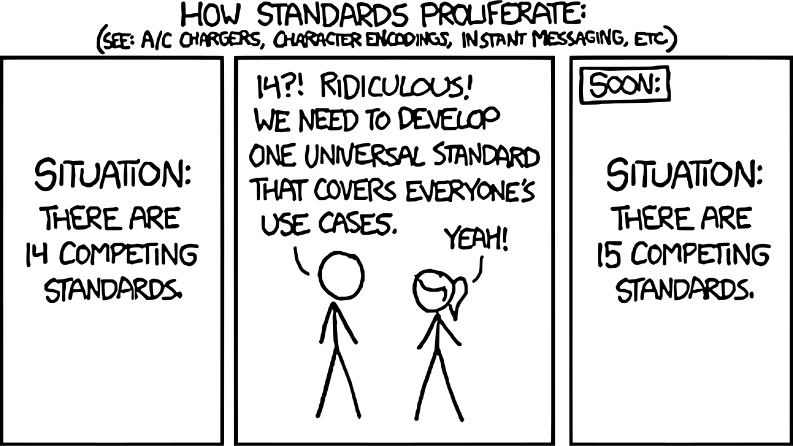
\includegraphics[width=\textwidth]{./figures/01/xkcd927.png}
	\caption[Proliferation of standards]{How standards proliferate. Reproduced from XKCD 927 (www.xkcd.com).}
	\label{fig:xkcd}
\end{figure}


\colorbox{yellow}{ [Other problems to mention?]}

The solution to this fragmentation is not an easy feat, and several strategies could be implemented to alleviate the issue. The first milestone is, simply put, write good documentation: time-tested protocols, which detail the software and versions used in each step are of utmost importance. If files need to be exchanged and/or edited along the process, these editions must be noted too. Of course, multiscale protocols are only a patch and do not solve the background problem: fragmentation. In this matter, several software-only attempts have been made throughout last decades and will be further detailed in \autoref{chap:05}.

\subsection{Missing or partial structural data}
% \addcontentsline{toc}{subsection}{Missing or partial structural data}
modeling a compound or structure usually requires a good enough starting point, which depends on the type of structure. For example, building a small molecule like a drug or a catalyst has nothing to do with obtaining a macromolecular structure.

To work with small compounds, researchers usually draw a 2D depiction in software like ChemDraw $ \{ $ $ \} $  and then obtain a 3D structure out of it. Sometimes, the 2D->3D conversion is not trivial and a 3D model is sketched by hand in GaussView $ \{ $ $ \} $ , Avogadro $ \{ $ $ \} $  or similar software. $ \{ $ $ \} $  The automatic procedures are good enough to provide a reasonable structure, but more often than not the final structure has been manually adjusted. If the system features many degrees of freedom, this can be tedious. A common alternative consists of performing high-temperature molecular dynamics simulations to navigate the conformational landscape. Once the researcher is satisfied, the small compound can be directly minimized with quantum mechanics algorithms, but if the size is too large a short MD run might be required instead, in this case to ‘relax’ the structure.

Manually building molecules is feasible when the number of atoms is reasonable, but with macromolecular structures such as proteins or DNA this does not hold true. For this type of systems, the initial model will ideally come from experimental data such as atomic-resolution 3D coordinates obtained with X-Ray crystallography (XRC) or Nucleic Magnetic Resonance (NMR). However, even if a 3D model is available, a part of the structure can be missing, which is very common with flexible loops. If that is the case, the researcher must model the missing parts by rebuilding the known sequence with sensible spatial restraints. In other cases, the full 3D structure might be missing, but similar structures (homologs) are available and can be used as a template -the perfect application for homology modeling (see \autoref{chap:02}). In both cases, the resulting structures should be quality-assessed with utilities like ERRAT $ \{ $ $ \} $  or PROSESS $ \{ $ $ \} $ . Sometimes, MD simulations are needed to check if the structure is stable along time, which can be also recommended in some other cases like XRC models with high B-Factors or deviant multi-model NMR structures.

Even with a proper protein structure, if the study features custom ligands, obtaining a good candidate for further steps in the protocol is not as simple as one might think. Assuming the required ligand structure is available, a regular protein-ligand docking simulation can provide an initial guess of the complex, but this is usually processed with long MD runs to assess the stability of the interactions. However, if the ligand is not known and must be designed from scratch, there is no consensus strategy. Two common approaches involve: (1) creating a library out of ligands that exhibit the needed chemical features using a reverse pharmacophoric approach, which then would be screened to assess their stability within the protein; (2) applying topology operators during the docking simulation itself using topology operators to dynamically build the ligand out of smaller fragments. The latter has been applied successfully in one the programs presented in this thesis, and will be discussed in \autoref{chap:06}.

For larger scale systems like viral capsids or lipid bilayers, which can feature millions of atoms, building a starting structure can be daunting at first, but fortunately they all exhibit some kind of symmetry that can be used to assemble the full structure out of the involved subunits with specialized software. $ \{ $ $ \} $

\subsection{Living with metal ions in macromolecules}
% \addcontentsline{toc}{subsection}{Living with metal ions in macromolecules}
One of the most exciting areas of molecular modeling sits at the frontier between organometallics and biochemistry, two fields that have been studied separately in computational chemistry for decades now. Globally, chemists exploit their features differently and, as such, present different computational challenges. Traditionally, organometallic systems feature a reduced number of atoms and accommodate transition metal centers within their structure, whose exotic electronic behavior can only be accurately computed with quantum chemistry approaches. Studies on biological problems such as the early work on folding of peptides and proteins had to face a larger number of atoms (hundreds or thousands) from the beginning, forcing the authors to use classical mechanics approaches to deal with the added dimensionality after realizing that the electronics of the system were not very important in that process.

However, metals do take part in biological processes as mainstream as oxygen transportation and muscle contraction. As such, the existence of metalloproteins cannot be neglected by the modeling community, who should bring these two areas together in a more seamless experience. Given the diverging efforts accumulated for decades, the gap is not easily overcome, but some solutions exist. Depending on the properties to study, one can resort to different approaches, as detailed below.

\subsubsection{Quantum Mechanics}
% \addcontentsline{toc}{subsubsection}{Quantum Mechanics}
Since quantum mechanics deal explicitly with the electronic shells of atoms, the immense diversity of electronic configurations of metal ions does not represent a problem. If such, the only challenge this might present is choosing the adequate functionals, basis sets or starting-point structures.

The challenge is more technical than scientific. While advances in DFT theories and hardware architectures allow us to deal with up to 500-atom systems in feasible timescales, this is still far from the number of atoms usually present in protein structures. For this, hybrid QM/MM studies are more adequate: the QM layer is responsible for dealing with the metal and its surroundings (at least, the first coordination sphere), while the, comparatively cheap, MM layer governs the rest of the structure. Even with this approach, time-dependent schemes still represent a huge computational effort, not to mention the difficulties in setting up the system adequately. One must still deal with layer boundaries effects or the parameterization needed for the MM calculations.

\subsubsection{Molecular Mechanics}
% \addcontentsline{toc}{subsubsection}{Molecular Mechanics}
Sometimes, QM is not necessary for a modeling study, since the metal might only play a structural role without exhibiting reactivity. In these cases, it is more interesting to gather an insight into the structural behavior of the system along time. Nowadays, for macromolecular systems, this is only feasible with molecular dynamics approaches, which require accurately parameterized force fields. Traditionally, force fields were developed to solve problems existing with proteins, nucleic acids and organic compounds $ \{ $ Lifson, Allinger, and so on; lots of references in the UFF paper$ \} $ , so historically transition metals have not been considered in force field development. Additionally, they present complexities not present in the reduced set of organic elements: several coordination geometries, different charge states, exotic polarizable behavior... As a result, dealing with metals in molecular mechanics is usually challenging. One must choose between (1) not considering them at all, (2) using a low-accuracy general-purpose force field, or (3) facing the tedious process of parameterization.

Ignoring or removing the metal ions can be acceptable in certain cases where they do not play a crucial role in the structure or dynamics of the system, but that is rarely the case. While general purpose force fields are numerous and heavily used, they mostly target organic compounds (such as CGenFF,\cite{Vanommeslaeghe2009} GAFF,\cite{Wang2004} Tripos 5.2 force field\cite{clark1989}). Only some include parameters for metal ions: UFF (for Universal Force Field,\cite{rappe1992} MMFF\cite{halgren1996}) covers the full periodic table, but Dreiding\cite{Mayo1990} only contains parameters for Na, Ca, Zn and Fe. While useful for organic chemistry, they are not as used in simulations including biological systems $ \{ $ $ \} $ , since they tend to rely on the Lennard-Jones based ‘nonbonded model’ $ \{ $ $ \} $ .

A feasible alternative for bio-containing systems is the so-called ‘bonded model’, which treats metal ion interactions with both bonded and non-bonded parameters; i. e., the metal is assumed to bond to some residues. Some of the protein-oriented force fields like AMBER $ \{ $ $ \} $  or CHARMM $ \{ $ $ \} $  distribute force field extensions for some of the most common metal ions in proteins, such as hemo-coordinated iron, but mainly as examples on how custom parameters can be added in the software. These types of force field extensions are only valid for the context where the parameters were obtained; i. e., the iron parameters for the heme groups will not reproduce the behavior of iron in other organic contexts such as ferrocenes. While the file format is easily understood, the values of the parameters are not easy to obtain: one has to resort to experimental data or \textit{ab initio} calculations to get adequate constants for bonded (distances, angles, dihedrals) and nonbonded (electrostatic, Van der Waals) interactions. While an expert user can decide to obtain those values manually, the process is not trivial and some protocols and tools have appeared to assis. They are mostly based on the Seminario’s method and his FUERZA software, \cite{Seminario1996} such as MCPB, MCPB.py,\cite{li2016} VFDFT.\cite{zheng2016} Recently, alternative approaches based on machine and statistical learning, \cite{fracchia2017,li2017b} and non-Seminario strategies\cite{Burger2012, allen2017} have also appeared, but the principle remains the same: extract the information from \textit{ab initio} calculations. Given the complexity of the task, some specific force fields have arisen lately to provide parameters for certain metals:

\begin{itemize}
	\item \href{http://onlinelibrary.wiley.com/doi/10.1002/9780470125830.ch2/summary}{http://onlinelibrary.wiley.com/doi/10.1002/9780470125830.ch2/summary}

	\item \href{http://onlinelibrary.wiley.com/doi/10.1002/jcc.10171/full}{http://onlinelibrary.wiley.com/doi/10.1002/jcc.10171/full}

	\item \href{http://pubs.acs.org/doi/abs/10.1021/ic00068a012?journalCode=inocaj}{http://pubs.acs.org/doi/abs/10.1021/ic00068a012?journalCode=inocaj}

	\item \href{http://pubs.acs.org/doi/abs/10.1021/jp046244d}{http://pubs.acs.org/doi/abs/10.1021/jp046244d}

	\item \href{http://pubs.acs.org/doi/abs/10.1021/ja00001a001?journalCode=jacsat}{http://pubs.acs.org/doi/abs/10.1021/ja00001a001?journalCode=jacsat}

	\item \href{http://onlinelibrary.wiley.com/doi/10.1002/jcc.20634/full}{http://onlinelibrary.wiley.com/doi/10.1002/jcc.20634/full}

	\item \href{http://onlinelibrary.wiley.com/doi/10.1002/pssb.201248460/full}{http://onlinelibrary.wiley.com/doi/10.1002/pssb.201248460/full}

	\item \href{http://pubs.acs.org/doi/abs/10.1021/ct400952t}{http://pubs.acs.org/doi/abs/10.1021/ct400952t}
\end{itemize}

A radically different strategy consists of mimicking the interactions of the metal site with positively-charged pseudoatoms strategically placed at around 0.9A from the metal nucleus following the vertices of the adequate coordination geometry. The Cationic Dummy Atom Model (CDAM) was introduced for Mn2+ ions by Aaqvist $\&$  Warshel in 1990\cite{aaqvist1990} and has been successfully implemented in further studies fore Zn, Mg, Ca, Fe, Co, Ni, Cu and more $ \{ $ duarte2014, 788, 790-795 in li2017$ \} $ . Among its advantages, once parameterized the CDAM approach is context-independent, but it forces a fixed coordination number and geometry on the modeled metal site.

The application of polarizable force fields (Fluctuating Charge methods, ABEEM, Drude oscillators and rods, induced dipoles, AMOEBA, PFF) or more exotic models based on Angular Overlap and Valence Bond Theory are also promising approaches, but the additional calculations incur in a big performance penalty when compared to other strategies and still require additional parameterization. Further details on the topic can be found in the extensive review published by Li and Merz Jr. in 2017.\cite{li2017}

\subsubsection{Lower levels of theory}
% \addcontentsline{toc}{subsubsection}{Lower levels of theory}
If the study at hand does not require a molecular mechanics treatment, such as docking studies of virtual screening approaches, the parameterization problem is usually not present or, at least, not that complicated. Docking studies, which try to accommodate small compounds within macromolecules, have not considered metals for years, since they were originally designed to find drug-like, organic compounds suitable for the pharmaceutical industry. Fortunately, over time some of the most popular docking packages have included strategies to deal with metals $ \{ $ FlexX$ \} $ , albeit sometimes they could only be part of the host (usually a protein), and not part of the probe (the ligand) $ \{ $ GOLD$ \} $ . To overcome the problem, approaches inspired in the Cationic Dummy Atom Model implemented in MM studies have been designed (‘H-bond trick’): in this case, the dummy atoms are hydrogen atoms that behave as a hydrogen bond donor, a chemical feature commonly implemented in docking software.

Other approaches involve considering the metal problem as a geometric optimization problem, restraining their position with distances, angles and dihedrals measurements. This strategy is partially implemented in homology modeling software like MODELLER, \cite{Sali1993} and is one of the main features of the developments presented in this thesis (detailed in \autoref{chap:03}).

In cheminformatics, explicit consideration of atoms is not as important and strategies like the pharmacophoric studies only have to consider metals as a custom type of interaction hotspot $ \{ $ johns2009,kawasuji2012,carcelli2014.pdf,yang2016$ \} $ . In QSAR, a catalogue of metal empirical properties is enough to build the dataset (QSAR $ \{ $ Fundamental QSARs for Metal Ions, John D. Walker, Michael C. Newman, Monica Enache, CRC Press; December 2012$ \} $ , especially in toxicity studies. \cite{enache2003,can2007,puzyn2011,gajewicz2014,pan2016}.


%!TEX root = ../dissertation.tex
\chapter{Materials \& Methods}
\label{chap:02}

\Lettrine{Computational chemistry} was first coined by Schleyer at a conference in 1966 to refer to Allinger’s work on molecular mechanics, separating it from other studies that would fall under the ‘theoretical chemistry’ category at that time. Nowadays, the term is broader and considers far more techniques. In fact, under the modern definition earlier works would be considered ‘computational chemistry’; albeit analog ones. In 1930, Kettering and more researchers in General Motors, built ball-and-spring models for several molecules and correlated their vibration modes with their Raman spectra. This work, titled ‘A representation of the dynamic properties of molecules by mechanical models’ could be considered one of the first ‘molecular modeling’ works.

\section{Origins of molecular modeling}
% \addcontentsline{toc}{section}{Origins of molecular modeling}
The birth of theoretical chemistry, from a quantum chemistry perspective, can be pinpointed with the description of the Schrödinger equations in 1925-1926 $ \{ $ $ \} $ . The first application of quantum mechanics came a year later, in 1927, with the publication of Burrau’s studies on $H_{2}^{+}$\cite{burrau1927} and Heitler and London calculations on H2 $ \{ $ Heitler $\&$  London, 1927$ \} $ . The field began to grow rapidly (Teller $ \{ $ $ \} $ , Mulliken $ \{ $ $ \} $ , Born $ \{ $ $ \} $ , Oppenheimer $ \{ $ $ \} $ , Pauling $ \{ $ $ \} $ , Hückel $ \{ $ $ \} $ , Hartree $ \{ $ $ \} $ , Fock $ \{ $ $ \} $ $ \ldots $ ) and computational implementations of the new theoretical framework started to be feasible after the advances in computer technology during the late 40s $ \{ $ $ \} $ . In the 50s and 60s, several milestone papers were published, making for the first documented computational chemistry calculations (refer to $ \{ $ https://onlinelibrary.wiley.com/doi/10.1002/9780470125823.ch1$ \} $  and CCL conversation $ \{ $ http://www.ccl.net/cgi-bin/ccl/message-new?2018+04+19+002$ \} $  for further information). Also, non-quantum, classical approaches stemming from theoretical physics started to emerge, although not strictly dealing with chemistry problems. \cite{Alder1959,Gibson1960,Rahman1964}

By the 70s, several journals had appeared to target computational chemistry and the first quantum chemistry packages began to be distributed (including the first version of the now ubiquitous Gaussian $ \{ $ $ \} $ ). The available hardware back then only allowed for ab initio\footnote{ A model is said to be ab initio when it only considers the resolution of the first principle equations (Schrödinger’s), without support from experimental observations. Empirically derived models do take these observations into account, very often as a workaround to avoid solving the full equation system. When the two approaches are combined, those are semi-empirical methods.  } calculations of molecules as big as naphthalene and azulene (18 atoms). In those same years, molecular mechanics methods became more popular, especially with the contributions by Lifson’s CFF $ \{ $ Warshel1969, Hagler et al., 1974; Hagler and Lifson, 1974; Niketic and Rasmussen, 1977$ \} $ , Allinger’s MM series $ \{ $ Allinger1973, Allinger1977$ \} $ , Scheraga’s ECEPP potentials $ \{ $ Momany et al.,1975; Némethy et al., 1983$ \} $ , Karplus’ CHARMM,\cite{brooks1983} van Gunsteren’s GROMOS $ \{ $ 1978$ \} $  and others, proving the power of empirical parameterization. By the 80s, Computer Assisted Molecular Design (CAMD) was the new hype that would revolutionize the pharmaceutical industry $ \{ $ Next Industrial Revolution: Designing Drugs by Computer at Merck, Fortune cover 1981$ \} $ , and by the 90s it was clear that computational chemistry was broader than quantum chemistry. In the preface of Reviews in Computational Chemistry Volume I $ \{ $ Kenny B. Lipkowitz, Donald B. Boyd, 1990$ \} $ , editors acknowledge that:

\begin{quote}
	"[...] we do not view the terms theoretical chemistry and computational chemistry as synonymous. Computational chemistry sometimes involves application of computerized algorithms from quantum theory, but computational chemistry is certainly more than quantum chemistry [...]. Molecular mechanics, molecular dynamics, computer graphics, molecular modeling, and computer-assisted molecular design are other important aspects of computational chemistry [...]".
\end{quote}

Nowadays, molecular modeling encompasses techniques and strategies beyond what is traditionally considered computational chemistry (this is, quantum and molecular mechanics, mainly). While a brief overview was already given in \autoref{chap:01}, more details are needed to fully comprehend the applicability of each method. However, this chapter is not intended as a manual on any of these methods, but a reasonably complete introduction to the numerous molecular modeling manifestations.

% [FIGURE: Timeline of molecular modeling milestones] TODO!

\section{State of the art of molecular modeling }
% \addcontentsline{toc}{section}{State of the art of molecular modeling }
These light notions on the history of molecular modeling introduced a key concept in model categorization: the \textit{theory level}, an estimation of the complexity of the theory supporting the method, that while arbitrary, gives a quick understanding of the intricacies involved. Higher theory levels usually refer to highly accurate, computationally demanding methods that rely on complex mathematical models. Lower theory levels, on the contrary, refer to less accurate and computationally cheap methods relying on simpler models.

In addition to quantum mechanics and molecular mechanics, after decades of progress, the currently available modeling toolbox is a rather diverse set of software utilities that apply very different theories, simplifications and approaches to deal with very particular problems. There are also a lot of different areas where they can be applied, and depending on the originating field, a very different mindset has permeated into the model. The following pages will introduce the major families of software approaches in computational chemistry and molecular modeling. They will be listed in two major groups depending on the focus (energy description or search space exploration), and in descending order of level of theory, which, in practice, means going from high-accuracy to lower-accuracy methods.

Lists: https://www.click2drug.org/index.html, https://omictools.com/

\subsection{Methods focused on energy description}
% \addcontentsline{toc}{subsection}{Methods focused on energy description}
\subsubsection{Quantum Mechanics (QM)}
% \addcontentsline{toc}{subsubsection}{Quantum Mechanics (QM)}
The main idea behind quantum chemistry is that molecules and, by extension, all ordinary matter, can be viewed as composed only of positively charged nuclei and negatively charged electrons. Mathematically, this can be expressed with the time-independent Schrödinger equation:

\begin{align}
	H \Psi =E \Psi =T_{n}+T_{e}+V_{ne}+V_{ee}+V_{nn} \\ \tag{Time-independent Schrödinger equation}
\end{align}

, where $H$ is the Hamiltonian operator, $E$ is the total energy of the system, $T_{n}$ and $T_{e}$ are the kinetic energies of nuclei and electrons, respectively, and $V_{ne}$, $V_{ee}$ and $V_{nn}$ are the potential energy between nuclei and electrons, electrons against each other, and nuclei against each other, respectively. Solving this equation for any system would mean seeking the eigenfunctions and eigenvalues of that Hamiltonian.

The details of such resolution are out of the scope of this thesis, but some comments can be made about its practical effects. Since only one-particle and two-particle systems can be solved analytically, numerical methods are employed to approximate the solution for systems of 3 or more particles: the many-body problem. While not analytical, the same methods can be applied iteratively to any given precision; the only restraints are computational and time resources. As a result, some approximations have been developed over the years to simplify the equation solving process without much accuracy loss.

The first approximation to appear was the Born-Oppenheimer approximation. It relies on the big mass difference between nuclei and electrons. In hydrogen, the monoprotonic nucleus is already 1800 times heavier than the electron; for uranium, the nucleus/electron mass ratio goes up to 430,000. This leads to consider that, given the enormous mass difference, electrons and nuclei move in different time-scales: if the nucleus moves, the electrons would follow ‘instantaneously’. This means that the nucleus can be considered stationary for electronic timescales, and appear as parameters in the equation, greatly simplifying its solution.

Even with uncoupled motions, the dynamics of electrons are complex and require advanced computational methods. A significant simplification would be to treat electrons as independent from each other by introducing a ‘independent-particle’ model, either by neglecting all interactions altogether, or, even better, by introducing an average interaction factor: the Hartree-Fock (HF) theory. In HF methods, electronic interactions are not explicitly described, but with a large basis set$\ast$  99$\%$  of the energy can be described by the HF wave function. The difference between the energy predicted by (Restricted) HF calculations and the real energy is called ‘electronic correlation’, which in certain chemical phenomena is key to obtaining accurate predictions. As a result, three main strategies have been developed to calculate it explicitly: Configuration Interaction (CI), Many-Body Perturbation Theory (MBPT) and Coupled Cluster (CC).

Evidently, these methods involve extra computational complexity, so in some cases, more aggressive approximations have been applied. This is the case of semi-empirical methods, which instead of trying to resolve some of the most complex integrals, resort to experimental parametrization of the results. While it is true that this leads to less accurate results, they are way faster and, with sensible parameters, the difference can be neglected depending on the study at hand.

HF theory is not the only applicable approximation to simplify the many-electron problem. In a way, Density Functional Theory (DFT) can be seen as a more efficient strategy to tackle the challenge. DFT is based on the Hohenberg and Kohn proof, which suggests that the ground state electronic energy can be determined completely by the electron density. This is, knowing the electron density leads to knowing the energy unequivocally. The only unknown here is guessing that correspondence, expressed as a functional\footnote{Not to be confused with a function: a function takes variables and produces numbers; a functional takes functions and produces numbers out of them.} or function of function(s). As opposed to HF methods, where the complexity of a wave function increases exponentially with the number of electrons, in Orbital-Free DFT, the electron density has always the same number of variables, independent of system size. However, describing the kinetic energy with a functional of the density is not accurate enough for the current demands of computational chemistry, so the most used approach today, based on the Kohn-Sham Theory, reintroduces orbitals to calculate the kinetic energy. This has three consequences: (1) accuracy is dramatically increased, (2) the complexity grows from 3 variables to 3N, (3) electronic correlation must be calculated separately.

Since HF-style orbitals now give 99$\%$  of the correct kinetic energy, the remaining energy can be absorbed in the correlation term, which is still calculated through an unknown functional. Even with higher complexity (N->3N) than Orbital Free DFT, it still less complex than the HF methods that explicitly consider electronic correlation. Thus, KS-DFT methods are generally preferred: the offer a computational cost similar to HF theory, but with the possibility of providing more accurate results. They need a good exchange-correlation functional, though, which can only be obtained exactly for the free electron gas; for other cases, approximations must be employed, like local-density (LDA), local spin-density (LSDA) or generalized gradient (GGA, meta-GGA) approaches.

All these methods are applied to solve the time-independent Schrodinger equation; this is, to obtain the energy of a system with given coordinates. If the dynamics of the system (i.e. evolution along time) must be studied, the time-dependent equation must be solved, which involves highly complex calculations to obtain reasonable accuracy. With current resources, only di- and triatomic species can be simulated this way. Additional atoms would need to be frozen or treated classically.

A workaround would involve a semi-classical approach. In Ab Initio Molecular Dynamics (AIMD), electrons are treated quantum-mechanically, and nuclei, classically (Born-Oppenheimer Molecular Dynamics, BOMD). At each time step, a converged wave function is obtained and the corresponding nuclear gradients are used to propagate the time-evolution. However, for accurate results, one must resort to tightly converged wave functions (in BOMD) or very small timesteps (in Car-Parrinello Molecular Dynamics, CPMD).

\subsubsection{Force fields: Molecular mechanic, Molecular dynamics and Metadynamics}
% \addcontentsline{toc}{subsubsection}{Force fields: Molecular mechanic, Molecular dynamics and Metadynamics}
Depending on the phenomena under study, explicit consideration of electrons is not always necessary. If that’s the case, the Schrodinger equation can be bypassed and \textbf{the electronic energy can be written as a parametric function of the nuclear coordinates}. Those parameters are fitted to reproduce either experimental measurements or results obtained with higher levels of theory (i.e. QM). The set of parameters needed to write the set of equations is called ‘force field’, and the theory behind this strategy is called ‘Molecular mechanics’ (MM). Given the size of nuclei, these can be treated classically with Newton’s second law with sufficient accuracy, resulting in equations much simpler than their QM counterpart, which allow faster computations and, as a result, dealing with larger systems (tens of thousands of atoms). Neglecting the existence of electrons has some consequences, though: bonding information is lost and must be provided explicitly, rather than being an inherent result of the equation.

In MM, molecules are described by a ‘ball and spring’ model: atoms are abstracted as spheres of given radius and ‘softness’, and bonds have length and ‘stiffness’. In such an ensemble, the potential energy of the system can be described as the sum of several components: stretching, bending, torsions, non-bonding interactions (usually, Van der Waals and Coulomb), and a cross-term of the first three.

 \begin{align}
	E_{FF}=E_{stretching}+E_{bending}+E_{torsional}+E_{non-bonding}+E_{cross} \\ \tag{Force field energy}
\end{align}

If each of the terms can be expressed as a function of the coordinates for the involved atoms, the potential energy can be obtained, and geometries and relative energies can be calculated by optimization. Thus, all that remains is to obtain the parameters for each type of interaction involved in the system under study. Fortunately, most molecules can be described as a composition of a small set of functional subunits or groups, the properties of which rarely change. For example, all \texttt{C=O} bonds are around 1.22 \AA long. Instead of having to parameterize each type of atom and bond for each type of molecule, these similarities allow to construct set of parameters with reasonable easiness, in principle.

As opposed to QM, these equations can be solved efficiently enough to consider time-dependent analysis. If one takes the force field equations and calculates the resulting forces and velocities, the position of the atoms can be figured out with high accuracy if the timestep is small enough (i.e. in the same order of magnitude as the smallest perturbation studied: hydrogen vibration, in the order of femtoseconds). This strategy gives rise to a field called Molecular Dynamics, which allows to study the behavior of molecules along time. Modern computer architectures allow to resolve each timestep around 10\textsuperscript{8 }times daily! Processes involving seconds in real-life can be calculated within a month.

Gaining access to such magnitudes allows to calculate properties not available in other higher levels of theory: conformational changes, binding pathways, or thermodynamic magnitudes such as free energy. However, in those calculations the potential energy surface (PES) must be well-sampled. Several methods account for this issue, such as metadynamics (MTD), umbrella sampling or adaptively-biased MD. In the case of MTD, the system is assumed to be describable by a few collective variables or reaction coordinates, which are then explored in such a way that revisiting sampled states is discouraged.

\subsubsection{QM/MM}
% \addcontentsline{toc}{subsubsection}{QM/MM}
Dealing with big systems (more than 300-500 atoms) with QM techniques is not feasible due to computational restraints. In some cases, though, only a subset of the system actually needs explicit consideration of the electrons. One strategy would consist of pruning the nonimportant parts, replacing them by smaller functional units which would keep the system’s $``$chemical identity$"$ .

In other studies, like enzyme reactivity, the nonreactive part of the enzyme is assumed to be important in keeping the active site conformation, and as such, cannot be pruned out. While some authors do model enzyme reactivity with a prune-and-freeze strategy $ \{ $ Himo$ \} $ ,\ a large part of the research community prefers to consider all the protein in the calculation.  This can be approached with QM/MM methods, in which the reactive atoms and its immediate surroundings are studied with QM, while the rest of the system is treated classically. The energy of the system is then calculated as a sum of the QM energy, the MM energy and the interaction between both.


\begin{align}
	E_{total}=E_{QM}+E_{MM}+E_{QM/MM} \\ \tag{QM/MM energy}
\end{align}


The independent QM and MM terms can be calculate straightforwardly as explained before, but deciding on how to calculate the interaction is not as intuitive. In general, three strategies can be applied: (1) mechanical embedding, which only considers bonded and steric effects; (2) electrostatic embedding, which also considers the electric field of the MM part; and (3) polarizable embedding, which also adds polarizabilities between the QM and MM parts. Even in the simplest case, mechanical embedding, technical difficulties may arise if a bond is cleaved by the QM/MM partitioning, which would require balancing the unpaired electrons in the QM part by adding a hydrogen ‘link’ atom invisible to the MM part. Similarly, the dangling bond in the MM part must be dealt somehow, normally adding the needed stretching, bending and torsional terms.

Mixing methods of different level theories for a single system is generalized in the ONIOM approach, which assumes additivity of the different ‘layers’. For two layers, it classifies the system in ‘model’ (the subset of the system which is dealt with a higher level of theory) and ‘real’ (the full model, including the ‘model’ subset). The ‘model layer’ is calculated both with the higher level of theory (usually QM) and the lower one (usually a force field), while the real layer is only calculated with the lower level of theory. Then, the energy is given as:

\begin{align}
  E_{ONIOM}=E_{high}^{real}=E_{high}^{model}-E_{low}^{model}+E_{low}^{real} \\ \tag{ONIOM energy}
\end{align}


Another intrinsic problem to QM/MM methods is the sampling. As the contribution of the MM part to the QM/MM energy is larger than the QM due to the number of atoms involved (around 100 in QM or 1,000-10,000 in MM), reported energy will be very sensitive to even small changes in the MM layer. As a result, when an energy profile must be calculated, the MM part is kept rigid during the whole process, which requires a carefully chosen initial structure to begin with. This usually involves a protocol where a long MD run is performed to obtain a representative snapshot of the simulation.

% [Figure: ONIOM scheme] % TODO!

\subsection{Methods focused on search space exploration}
% \addcontentsline{toc}{subsection}{Methods focused on search space exploration}
\subsubsection{Spatial exploration: normal modes $\&$  docking (protein-ligand docking)}
% \addcontentsline{toc}{subsubsection}{Spatial exploration: normal modes $\&$  docking (protein-ligand docking)}
Even with latest advances in computer architecture and software improvements to make the most out of it, some potential energy surfaces are too vast and complex to be explored efficiently with molecular dynamics, let alone quantum dynamics. While this might not apply in the next decade, techniques that take educated shortcuts to traverse broad conformational spaces are still necessary. This is particularly true in large molecules such as proteins, where structural fluctuations occur at very different time scales and amplitudes: local motions take place are fast and short (10\textsuperscript{-15} to 10\textsuperscript{-1}s, 0.01-5 \AA), and collective motions are slow and long (10\textsuperscript{-9} to 1s, 1-10 \AA). This category is too broad to be analyzed exhaustively, but two approaches can be highlighted due to their popularity: normal modes analysis (NMA) and docking procedures.

In NMA, slow, collective motions of a molecular structure can be approximated through the composition of its independent (normal) harmonic oscillations (modes). NMA approach is parallel to MM in its theoretical support, meaning that bonds are replaced by ‘springs’ or harmonic oscillators. As a result, the mathematical treatment consists of finding the eigenvalue of each coupled oscillator, which is simple enough to be calculated efficiently for thousands of atoms. In fact, there is no obligation to treat each atom and bond independently, as nearby atoms can be grouped together in a new body to reduce the needed number of oscillators (coarse-grained NMA). All these approximations allow dynamic insights on the movements of a macromolecule without the technical limitations of MD, which require long runs to observe slowest motions. Since NMA does not consider time at all and only requires an initial structure on which to compute the normal modes, the vibrations obtained only apply to that particular conformation. In other words, only the local potential energy wells are explored, which can provide a short-sighted analysis if no other conformations are assessed.

Recognition processes involve large conformational changes and are key in research areas such as drug development or metabolic studies. Again, MD principles should be able to simulate them with long runs, and would definitely be the way forward in the near future,\cite{devivo2017} but since the 90s a different shortcut was devised. Docking techniques were developed to describe feasible binding modes of small molecules (ligands) within a bigger macromolecule (the host, which is normally a protein). To do that, potential binding pockets in the host are explored explosively by placing the ligand in random orientations and positions (rigid body transformations), contemplating some internal flexibility if necessary (through torsions in the small molecule or rotamer exchange for the side chains in the protein), and finally assessing their non-bonding interactions. Since the spatial landscape needs to be explored efficiently, with thousands of attempts before finding a good pose, the energy representation is often cruder than in higher levels of theory in honor of speed and efficiency: the scoring function. While in principle it could use a full MM force field $ \{ $ $ \} $ , most popular approaches resort to simplifications, like knowledge-based parameters obtained out of structural databases $ \{ $ PDB$ \} $  or empirical evidences $ \{ $ $ \} $ . Other approaches resort to shape complementarity between the Van der Waals surfaces of the involved molecules and, more recently, to Artificial Intelligence (AI) deep learning techniques $ \{ $ $ \} $ .

Docking techniques can also involve other type of molecules, like protein-protein or protein-nucleic acid studies. In this variant, more approximations are needed due to the broader conformational space involved, like only considering rigid-body transformations.

\subsubsection{Chemogenetic exploration (assess mutation stability, chemical functionalization$ \ldots $ )}
% \addcontentsline{toc}{subsubsection}{Chemogenetic exploration (assess mutation stability, chemical functionalization$ \ldots $ )}
Of all the techniques detailed until know, only QM studies allow topology changes like bond breaking or creation. This is, when dealing with MM, NMA or docking, most approaches will assume that the starting set of atoms and their connectivity will be the same during the whole simulation. As a result, to assess different variants of the same compound one must run the same protocol separately for each variant.

The most popular technique employing this strategy is virtual screening, which essentially performs docking calculations for massive datasets of drug-like compounds. In most implementations, the database must be built beforehand and the chemical space is only explored by trying different entries in the dataset. This is, no algorithmic modification of the structure is done during the simulation. With big enough datasets, sampling should not be a problem, but some studies point out that the chemical space explored this way is very limited $ \{ $ mapa de calor usado en el master$ \} $ .



\begin{itemize}
	\item https://www.sciencedirect.com/science/article/pii/S0079610714000960

	\item https://www.nature.com/articles/nrd.2016.213

	\item https://www.thieme-connect.com/products/ejournals/abstract/10.1055/s-0034-1396322

	\item https://pubs.acs.org/doi/abs/10.1021/ar500432k

	\item https://www.nature.com/articles/nmeth.3493

	\item https://link.springer.com/article/10.1007/s10822-014-9760-0

	\item https://www.ncbi.nlm.nih.gov/pmc/articles/PMC5538041.2/
\end{itemize}

Some software projects do attempt to explore the chemical space algorithmically, like $ \{ $ cite a few here$ \} $ , but they still struggle to find mainstream usage in the pharma industry. The implemented approaches often resort to chemical synthesis guidelines like CLICK chemistry\cite{durrant2009} or graph abstractions.\cite{andersen2014} This can be useful in docking calculations that wish to account for some chemical variability in the ligands assessed or rational design of potential inhibitors.

Since protein-ligand docking studies involve at least two molecules, it makes sense to investigate chemical variability in the host. While the theoretical chemical space available in proteins is huge due to the number of atoms alone, fortunately is more constrained: all proteins are chains of the same 20 residues or amino acids. Hence, assessing possible variations \textit{only} involve changing one particular residue for another of the remaining 19. It seems simple at first, but the possible variations explode exponentially with chain length, which means that even for small peptides of around 30 residues it results in an unfathomable number: $ 30^{20} $ or around $ 3.5·10^{29} $ (see fig. \ref{fig:chemicalspace}). Subsequently, only a few positions are studied and the variations applied are somehow rational and studied beforehand. Some tools exist to evaluate the potential consequences of a mutation in a protein, which can help discard destabilizing changes $ \{ $ PoPMuSiC$ \} $  before doing more intense computations. After all, only one change in a key residue can alter the final structure dramatically $ \{ $ $ \} $ .

\begin{itemize}
	\item https://www.icr.ac.uk/blogs/the-bigger-picture/page-details/exploration-and-exploitation-of-potential-drug-space-using-computers
\end{itemize}

\begin{figure}[H]
	\includegraphics[width=\textwidth]{./figures/02/chemical_space.png}
	\caption[Chemobiological spaces]{
		In any study on protein-ligand interactions, considering sequence mutation of protein scaffolds, each with its possible sidechain orientations, already produces a combinatorial explosion. Taking different possible ligands into account adds one more dimension to the search space. (Reproduced from \textit{Rodríguez-Guerra, J., Alonso-Cotchico, L., Sciortino, G., Lledós, A., $\&$  Maréchal, J. D. (2018). Computational Studies of Artificial Metalloenzymes: From Methods and Models to Design and Optimization. Artificial Metalloenzymes and MetalloDNAzymes in Catalysis: From Design to Applications, 99-136}. $ \{ $ $ \} $ ).
	}
	\label{fig:chemicalspace}
\end{figure}

\subsubsection{Model/topology building}
% \addcontentsline{toc}{subsubsection}{Model/topology building}
Up to this point, it has been assumed that the molecular modeler had all the needed structures ready for analysis and simulation, but unfortunately that is not always the case.

In QM studies, when only small molecules are studied, manual building of the model can be contemplated as a possibility using a graphical interface $ \{ $ GaussView, Avogadro$ \} $ , but when the model grows, the possible orientation of rotatable bonds or the configuration of the subunits can be a daunting task to solve manually and even a stopping barrier in the research. Additionally, in some cases, the initial structure is only conceived as a 2D depiction with ChemDraw or similar software, which has to be transformed into a 3D model. This a fairly common process, and as such most software suites include a 2D->3D converter $ \{ $ $ \} $ . However, additional refinements are normally required afterwards.

In macromolecular studies where the conformational space is untreatable, experimental data is needed beforehand, like X-Ray Crystallography (XRC) or Nuclear Magnetic Resonance (NMR). These techniques provide density maps to which, with adequate refinement and post-processing using specialized software $ \{ $ CCP4, Phenix$ \} $ , 3D structures are fitted. After validating the quality of the resulting model with ERRAT or similar protocols $ \{ $ $ \} $ , these are then usually submitted to specialized databases like Protein Data Bank (PDB) $ \{ $ $ \} $ , from which the researchers can download the needed files for modeling the required system. Most of the time, files downloaded from PDB must be edited to remove experimental artefacts like duplicate positions of some atoms, protonate the residues at the desired pH by inferring the pKa of each one $ \{ $ Reduce, PropKa, \textit{addh}$ \ldots $ $ \} $ , or reproduce the biological assembly of the structure $ \{ $ SIENA, UCSF Chimera$ \} $ .

While the Protein Data Bank holds almost 140,000 structures readily available for everyone, not every protein is there. Sometimes, the structure is partially missing due to experimental limitations or even totally absent. In those cases, the model must be built from scratch. The folding problem is still unsolved and guessing the tertiary structure out of the sequence of amino acids is very challenging, but workarounds exist to work with available data. For example, if the protein that needs to be modeled has an already characterized homolog in the database, their sequence alignment can be used as a template to reconstruct a good structure. This technique is called homology modeling and its accuracy grows when multiple sequence alignment (MSA) are available. Since the final model is only an interpolation of closely related structures, some external validation is needed. In MODELLER, one of the most popular packages for homology modeling, several scoring functions to assess the quality are available. Additionally, a series of web services can be found to help in the task $ \{ $ ERRAT, QMEAN, APOLLO$ \ldots $  More on \href{https://www.click2drug.org/directory\_HomologyModeling.html}{https://www.click2drug.org/directory\_HomologyModeling.html}$ \} $ .\

\subsubsection{Cheminformatics}
% \addcontentsline{toc}{subsubsection}{Cheminformatics}
All previous techniques relied on 3D structural models of the involved compounds, but there are molecular modeling techniques that do not need to rely on that information to produce useful results.

Cheminformatics are mainly concerned with the creation and maintenance of small compound databases with support for indexation and similarity searches. The main exponent of cheminformatics approaches is probably Q\/SAR techniques.

Quantitative Structure-Activity Relationship (Q\/SAR) studies apply classification or regression statistical techniques to predict experimental observables from basic molecular descriptors. The\ ‘activity’ under study can comprise different variables: biological activity of a drug-like compound, boiling point, potential reactivity, toxicity$ \ldots $  All Q\/SAR methods are based on the structure-activity relationship (SAR) assumption: similar compounds will have similar activities. The main issue is how to measure that similarity: number of atoms, functional groups, connectivity$ \ldots $   As in all statistics, large datasets are needed to obtain valid results. The first step in Q\/SAR studies is to train the statistical model with a huge library of compounds. Once the model is trained, it can be used to predict the activity of a compound originally not present in the library.

Q\/SAR input data do not provide 3D-structural data (with the exception of the 3D-Q\/SAR variants), but 2D-topological information. These are normally supplied with special character strings called SMILES (Simplified Molecular Input Line Entry Specification) $ \{ $ $ \} $ , which can describe compounds unambiguously without resorting to explicit coordinates specification. SMILES strings work by enumerating the atoms involved in a molecule with their element symbol, except hydrogen, which is usually implicitly considered. Simple bonds are assumed between linearly adjacent elements. If a ramification occurs, it must be specified with parenthesis. Numeric tags are used to signal the starting and ending atoms of cyclic substructures (see fig. \ref{fig:smiles}). For example, butane would be represented as \texttt{CCCC}, while D-glucose would be \texttt{C(C1C(C(C(C(O1)O)O)O)O)O}.


\begin{figure}[H]
	\begin{center}
	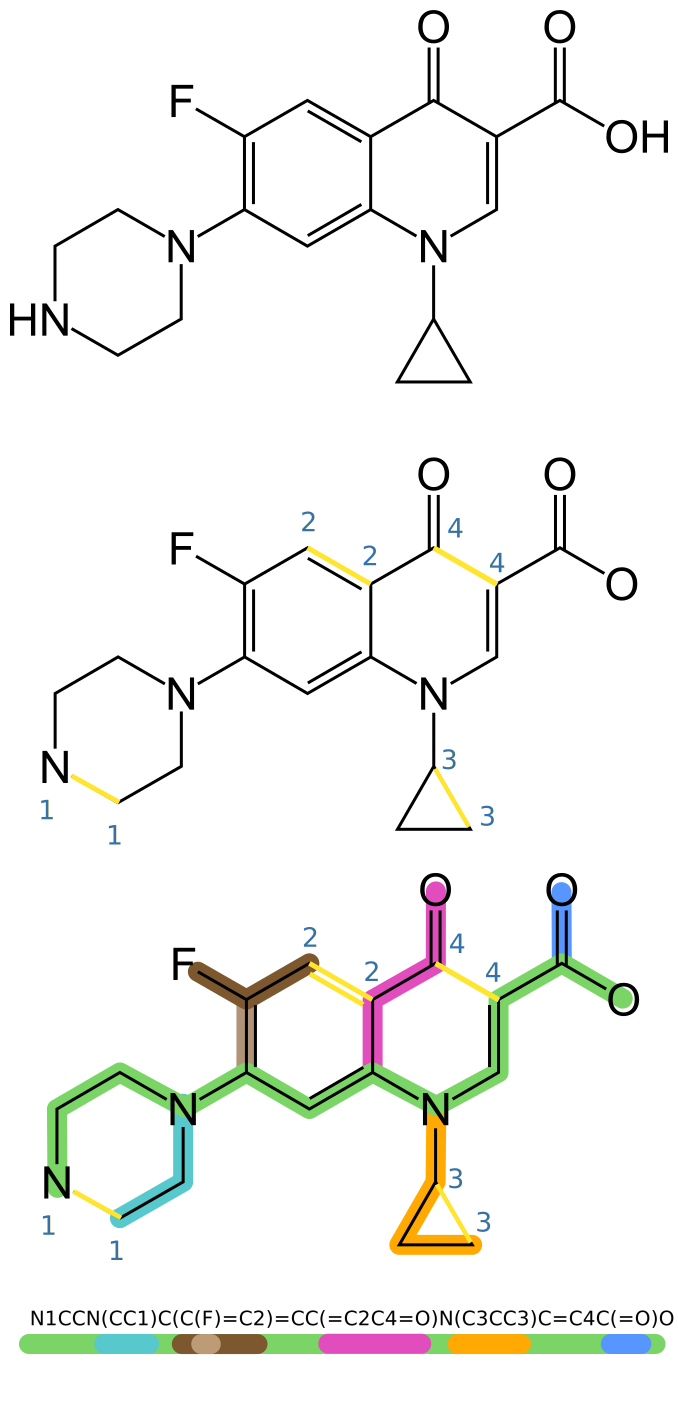
\includegraphics[height=0.9\textheight]{./figures/02/smiles.png}
	\end{center}
	\cprotect\caption[SMILES notation]{SMILES notation can depict a substituted aromatic ring as linear chains with branches. In this case, 3-cyanoanisole is being written as \texttt{COc(c1)cccc1C$\# $N}.}
	\label{fig:smiles}
\end{figure}


\section{Optimization problems in modeling}
% \addcontentsline{toc}{section}{Theory behind the concept: Optimization problems}
\subsection{Mathematical optimization and numerical methods}
% \addcontentsline{toc}{subsection}{Mathematical optimization and numerical methods}
Most of the procedures used to rapidly identify physically sound initial models of a molecular system stand on finding the way to ally the exploration of wide conformational spaces and the adequate guiding variables. In math speech, this is territory of optimization problems for non-smooth surfaces.

Mathematically speaking, an optimization problem consists of, given a function $ f $ that connects a set $ A $ to the set of real numbers, finding an element $ x_{0} $ in A such that $ f(x_{0}) \leq f(x) $ for all $ x in A $  (minimization), or such that $ f(x_{0}) \geq f(x) $ for all $ x in A $ (maximization).

\begin{align}
	Given ~~ f:A \rightarrow R \nonumber \\
	Sought: ~ x_{0} \in A ~ such ~ that ~ f(x_{0})  \leq f(x) ~,~x \in A ~~~ ( minimization ) \nonumber \\
	~~~~~~~~~ or: x_{0} \in A ~ such ~ that ~ f(x_{0})  \geq f(x) ~,~x \in A ~~~ ( maximization )
\end{align}

$ f(x) $  is normally called the objective function, loss function or cost function for minimization problems, utility function or fitness function for maximization problems or, depending on the field, energy function or functional. However, all optimization problems can be expressed as minimization problems, negating  $ f(x) $  if the problem is to be maximized.

The domain  $ A ~ of ~ f $ is usually named the ‘search space’ or the ‘choice set’, and each possible value of  $ A $  is called a candidate or feasible solution.  $ A $  is normally a subset of  $ R^{n} $ , as defined by equality and/or inequality constraints. The optimization definition can be extended to be subject to inequality and equality constraints, expressed as:

\begin{align}
	optimize_{x}~~~~~~~ f(x) \nonumber \\
	subject~to~~~  g_{i}(x)  \leq 0,~~ i=1,  \ldots ,m \nonumber \\
	~~~~~~~~~~~~~~~~~~~~~~~ h_{j}(x) =0,~~ j=1,  \ldots ,p
\end{align}

, where  \( g_{i}(x)  \)  are the inequality constraints,  \( h_{j}(x)  \)  are the equality constraints, and  \( m \)  and  \( p \)  are greater than 0. If  \( m \)  and  \( p \)  are equal to zero, the definition falls back to the unconstrained optimization problem.

Depending on the form of the function being optimized and the specified constraints, several categories emerge, like convex or nonlinear optimization problems. In convex optimization, when f, g and h are either convex (minimization) or concave (maximization). This includes linear functions, defining the field of linear optimization. Nonlinear optimization deals with functions that cannot be written as linear expressions, which usually makes the problem harder.

Solving this type of problems was initially studied by Fermat and Lagrange, who applied calculus-based formulae to identify optimum solutions. However, not all optimization problems can be solved analytically and, in fact, for some complex problems is usually easier (and faster) to compute numerical solutions iteratively until a convergence threshold is met. This approach was initiated by Newton and Gauss, and since then many applicable algorithms have been devised throughout the latest decades. A few will be highlighted for illustrative purposes.

\subsubsection{Steepest descent and conjugate gradient}
% \addcontentsline{toc}{subsubsection}{Steepest descent and conjugate gradient}
To go down a smooth mountain, one simply takes steps in a direction towards the valley. There’s a lot of possible directions, but skilled mountaineers usually take the fastest: the steepest side. Climbing down that mountain can be expressed as finding the minimum of a convex three-dimensional function, so figuring out which direction we should take in every step is a matter of finding the gradient of that function at that point.

A gradient is the $n$-dimensional generalization of a single-variable derivative, so instead of returning a scalar, it returns a vector. If derivatives gave us the rate of change of a function, gradients will tell the direction in which the function will experience the greatest change. In this three-dimensional problem, the gradient vector will point to the next step. By taking little steps in the direction pointed by the gradient, we will eventually get to the minimum.

This is what the steepest descent algorithm does, but it can progress very slowly in almost ‘flat’ regions of the function. A similar method named conjugate gradient uses a similar approach, but the search direction is computed in a smarter way, making sure that the direction is orthogonal to the previous step gradient and the current one. It requires more operations, but the performance towards the optimum is better and usually worthy.

Since these methods only compute $f(x)$ and $f’(x)$ (first derivatives), they are called first-order methods.

\subsubsection{The Newton and quasi-Newton algorithms}
% \addcontentsline{toc}{subsubsection}{The Newton and quasi-Newton algorithms}
Newton numerical algorithms are similar to SD and CJ methods, but compute an additional differentiation step to use the information provided curvature of the function. This makes each iteration more expensive, but with certain functions fewer iterations might be needed (see fig. \ref{fig:gradientdescent}).

Second derivatives can be generalized as Hessian matrices for problems of higher dimensions, but this can get very expensive to compute. As a result, several derived methods, called quasi-Newton methods, include alternative methods to compute it or supply equivalent information, like directly computing the inverse with numerical methods, updating it with successive gradient vectors$ \ldots $  Due to its performance, one of the most popular quasi-Newton algorithms is the BGFS algorithm (for Broyden, Fletcher, Goldfarb, Shanno) and its limited memory version L-BGFS.



\begin{figure}[H]
	\includegraphics[width=\textwidth]{./figures/04/gradientdescent.png}
	\caption[Gradient descent vs Newton's optimization]{A comparison of gradient descent (green) and Newton's method (red) for minimizing a function (with small step sizes) starting with $ X_{0} $. Global minimum is $ X $. Newton's method uses curvature information to take a more direct route.}
	\label{fig:gradientdescent}
\end{figure}

\subsubsection{The simplex algorithm}
% \addcontentsline{toc}{subsubsection}{The simplex algorithm}
Described by Dantzig during the World War II, this algorithm solves linear optimization problems by expressing functions and constraints in a n-dimensional generalized polyhedron called polytope. The algorithm shows that the optimum point of a convex polytope is one of the vertices and can be found by iteratively traversing the edges.

\subsection{Heuristics: thinking abstract but practical}
% \addcontentsline{toc}{subsection}{Heuristics: thinking abstract but practical}
While all these numerical methods are very different in nature, they still perform the same kind of tasks: exploration, evaluation and selection. This is, they generate a candidate solution (exploration), solve the equations and assess how far they are from the exit condition (evaluation). Selection is often so trivial in scalar functions that is not even considered as a separate step. When it comes to the selecting a new candidate solution of all the possible in the search space, if $f(x)$ points to a scalar space, selecting $f(x_{0})$ vs $f(x_{1})$ is just a matter of seeing which value is smaller (minimization) or greater (maximization). However, if $f(x)$ points to a n-dimensional space, the selection is not straightforward because $f(x_{0}) < f(x_{1})$ will be only defined if all the elements in $x_{0}$ are smaller than $x_{1}$. This subject is studied in multi-objective optimization.

In a simplified example, where we must find $f(x) = 0$ with $f(x) = ax + b$, ‘generating new candidate solutions’ would simply consist of assigning new values to x. While this can be done randomly until the solution is found, it’s usually more interesting to use a smarter approach. This what the gradients and hessian approaches provide: educated guesses towards finding the optima. However, they still require an equation to be available. When several variables are analyzed and the relationship between them is not differentiable or, simply, unknown, other type of algorithms must be employed, like heuristics.

\subsubsection{Monte Carlo methods}
% \addcontentsline{toc}{subsubsection}{Monte Carlo methods}
In Monte Carlo methods are useful for studying problems that are characterized by a huge number of degrees of freedom but can be interpreted probabilistically. Since the expected value of an integral can be approximated by the empirical mean of a random sample, these methods allow to obtain numerical results by randomly sampling the search space. In the Metropolis variant, the sample is refined iteratively with random modifications that are either accepted or rejected depending on the new value of the sample or a random acceptance ratio.

For example, to minimize the potential energy of a molecule, random states can be generated by introducing small perturbations to the atomic positions that follow a Boltzmann distribution. The energy of the new states is evaluated and either accepted or rejected by comparing their energies with current mean of the sample. For example, those with smaller energies are usually included and accepted in the ensemble. For those with higher energies, they can still be included with some probability that depends on the chosen acceptance ratio. Being a Markov chain, the probability distribution for the next iteration will be reparametrized with the state of the current sample and the process will continue iteratively until convergence.

\subsubsection{Evolutionary algorithms}
% \addcontentsline{toc}{subsubsection}{Evolutionary algorithms}
Evolutionary algorithms (EA) can be explained as an extension to Monte Carlo’s: they also employ random generation of solutions as starting points, but following iterations employ biology-inspired heuristics to localize next candidate solutions. In each iteration, the ‘population’ of feasible solutions (individuals) are evaluated in the optimization environment, and each one is assessed a fitness score. Like in the Evolution theory, only the fittest will be allowed to survive (included in the sample for the next iteration).

Genetic algorithms (GA) are a special type of EA that implement ‘evolutionary’ heuristics inspired on chromosomic changes. By mimicking chromosomes during the meiosis, candidate solutions can exchange some of their variables (mating or recombination), and some can experience a random change in one or more variables (mutation). By iterating over this ‘sexual’ cycle, fitter and fitter solutions will be obtained.

\subsubsection{Machine learning }
% \addcontentsline{toc}{subsubsection}{Machine learning }
Artificial Intelligence and Machine Learning are very popular computer science fields these days. Globally, they are algorithms that can ‘learn’ from their own ‘experience’ by extracting patterns and relationships out of the supplied data. They can be studied as non-linear statistical data modeling tools.

One of the hottest branches of Machine Learning are Artificial Neural Networks and, especially, Deep Learning. The implemented algorithms in these categories mimic the way neurons work in the brain. Like all mathematical functions, each ‘neuron’ produces an output that depends on the input. Many neurons are grouped together in layers and these layers are concatenated, having the output of one layer fed as the input of the next one. Layers can back-propagate, and modify the input of previous layers, like the feedback mechanism of the brain. Ultimately, this construction generates a huge set of self-adjusting equations that can optimize wide ranges of observations. For example, they are actively used in speech recognition, computer vision or artificial intelligence. The hype produced by its success in other areas made it permeate towards some areas of science where its application is controversial and less ‘fancy’ algorithms like random walks (Monte Carlo and similar) are equally performant $ \{ $ $ \} $ .

\todo[inline]{Maybe advance multiobjective optimization here?}
%!TEX root = ../dissertation.tex
\chapter{Objectives}
\label{chap:03}

\Lettrine{Multiscale} molecular modeling employs different modeling techniques and levels of theory, per definition. However, resorting to such a vast variety of software tools means they do not usually play well together. Being conceived by teams with different background and focus, this end up resulting in three common symptoms:

\begin{itemize}
	\item Most molecular modeling tools are designed as standalone pieces not meant to be part of broader, multistage protocols.

	\item They present unintentionally opinionated abstractions and problem-solving strategies that force users to recontextualize their problem for each tool.

	\item The files required are almost never compatible, which results in non-trivial format conversions or manual input, especially if data exchange is needed.
\end{itemize}

Subsequently, when a researcher faces a multiscale protocol, a series of technical issues unrelated to the scientific problem arise: files are not properly converted, software dependencies are not updated, the operating system is not supported anymore$ \ldots $  Molecular modeling is difficult enough by itself; there is no need to put additional barriers in the way.

The main motivation behind this thesis is to provide new software solutions to make technical and scientific barriers easier to overcome when it comes to molecular modeling and multiscale protocols. Several tools will be presented in the next chapters, each focusing on a specific part of the multiscale funnel. Two of them constitute the main projects of this thesis:

\begin{itemize}
	\item GaudiMM, described in \autoref{chap:04}, is a multi-objective optimization platform to provide reasonably sound models meant to be used as starting structures for subsequent stages down a multiscale protocol.

	\item Tangram suite, described in \autoref{chap:05}, is a collection of graphical interfaces for UCSF Chimera to bridge diverse molecular modeling tools in a single, intuitive user experience. This chapter also includes command-line utilities that were started as helper tools and ended up becoming independent projects on their own.
\end{itemize}

Finally, in \autoref{chap:06}, a collection of illustrative cases will be described in detail to prove their usage and applicability. These include toy examples that showcase the potentiality of GaudiMM, and a detailed computational insight on the counter-intuitive experimental observations found in multivalent enzyme inhibition studies.


%!TEX root = ../dissertation.tex
\begin{savequote}[0.6\textwidth]
	\itshape In the beginning, there was nothing. \\
	\itshape And God said, Let there be light. \\
	\itshape And there was light. \\
	\itshape There was still nothing, \\
	\itshape but you could see it a lot better.
	\qauthor{---Woody Allen}
\end{savequote}

\chapter{GaudiMM}
\label{chap:04}


\Lettrine{There} is an implicit restriction in multiscale approaches due to their own design. They are based on a sequential series of steps, which are chained one after another to answer the initial question. Each step must be resolved separately, which can potentially become a bottleneck or even a blocking step if the results are not successfully obtained.

% Indirectly, methods that suffer from insufficient sampling capacity can only operate with subregions of the system under study, deliberately ignoring details outside that region.

Instead of forcing a sequential protocol around a complex molecular problem, an alternative approach could be devised. If the panoply of existing modeling methods could be recruited on demand to work simultaneously on the same study, all of them could contribute to solve the problem, multiplying their strengths and compensating their weaknesses. Building this feature set into a robust and flexible platform would be very desirable for drafting molecular hypotheses and sketching proofs of concept.

GaudiMM is here presented to become such a platform. It takes the expressiveness and flexibility of Python to create a molecular design platform with unprecedented versatility. The rationale behind its concept can be summarized in three points:

\begin{enumerate}
	\item Its modular implementation allows to encapsulate separate methods in isolated entities that can work together through a well-defined programmatic interface, which also allows fast development of new extensions.

	\item It makes a clear distinction between the three main stages of any optimization process (exploration, evaluation and selection), which suggests a flexible way of rationalizing molecular modeling problems.

	\item It does not require prior knowledge of the importance of the variables that affect the system thanks to its multi-objective optimization capabilities.
\end{enumerate}

As a result, solving a molecular modeling problem is only a matter of choosing the appropriate modules in terms of which variables should be explored (cartesian coordinates, chemical spaces...) and which properties should be measured (geometries, energies...). In some cases, some rigor can be sacrificed in honor of obtaining good enough results to start working with. In other cases, the combination of methods will work synergistically towards the design of a novel methodology.

Following sections will describe: (1) the algorithmic and (2) implementation details of the platform, (3) how different combinations of modules allow diverse molecular modeling tasks, and (4) how to analyze the proposed results.

%%%%%%%%%%%%%%%%%%%% Table No: 1 starts here %%%%%%%%%%%%%%%%%%%%


\begin{table}[hbtp]
	\caption{GaudiMM: technical datasheet}
	\footnotesize
	\newcolumntype{R}{>{\hsize=.25\hsize\raggedleft\arraybackslash}X}%
	\newcolumntype{L}{>{\hsize=.75\hsize\raggedright\arraybackslash}X}%
	\newcommand{\tableheading}[1]{\multicolumn{2}{c}{\textsc{#1}}}
	\begin{tabularx}{\textwidth}{RL}
		\toprule
		%row no:1
		\tableheading{GaudiMM} \\
		\toprule
		%row no:2
		\textit{Description} & A modular optimization platform for molecular design \\
		\midrule
		%row no:3
		\textit{Requirements} & Python, UCSF Chimera, OpenMM, IMP, DSX, ProDy... \\
		\midrule
		%row no:4
		\textit{License} & Apache 2 \\
		\midrule
		%row no:5
		\textit{Download} & \href{https://github.com/insilichem/gaudi}{github.com/insilichem/gaudi} \\
		\midrule
		%row no:6
		\textit{Documentation} & \href{https://gaudi.readthedocs.io}{gaudi.readthedocs.io} \\
		\midrule
		%row no:7
		\textit{Citation} & J. Comput. Chem. 2017, 38, pp 2118–2126. DOI: 10.1002/jcc.24847 \\
		\bottomrule

	\end{tabularx}
\end{table}


%%%%%%%%%%%%%%%%%%%% Table No: 1 ends here %%%%%%%%%%%%%%%%%%%%

\section[Algorithmic details]{Algorithmic details: \\ multi-objective optimization \& NSGA-II}

GaudiMM is built on top of a multi-objective genetic algorithm (MOGA), NSGA-II, developed by K. Deb.\cite{nsgaii} It has been thoroughly tested and benchmarked in well-characterized multi-objective problems and is considered a prototypical MOGA.

As other optimization methods, this algorithm can be described in three main stages (exploration, evaluation and selection) that are executed iteratively until an exit condition is met (usually, convergence or maximum steps). Generating new candidate solutions or individuals is considered within the \textit{exploration} stage, and can be achieved by random attribute assignation or combining previously existing individuals. In the \textit{evaluation} stage, the candidates are assessed with different functions or objectives, each returning a scalar that represents a fitness score for that objective. Finally, the selection stage collects all the individuals and compares their vectorial scores to select the best individuals according to the Pareto dominance criterion (see \autoref{chap:02}).

In more detail, NSGA-II starts with the generation of a random set of potential solutions (\textit{individuals}) which comprise the so-called \textit{initial population}. This first set of individuals is then evaluated with one or more \textit{objectives} and each individual is assigned a \textit{fitness} score vector, the elements of which are the result of those cost functions. At this point, a small subset of the population is submitted to a round of random modification of parameters (\textit{mutation}) or exchanging some of their attributes (\textit{recombination}), and are then assessed by the same cost functions. Being random, the results of these variations can be better or worse than their preceding counterparts (parents). Finally, both the offspring and the parental generation ($ \mu $ +$ \lambda $ strategy) compete in the selection tournament, which will rule which ones will replace the initial population. After a number of iterations, the initial population will have evolved and, eventually, will end up providing reasonable solutions to the problem that represent a compromise between the analyzed variables (see fig. \ref{fig:nsga}).

\begin{figure} % FIXME!
	\vspace*{-1cm}
	\includegraphics[width=0.9\textheight,angle=90]{./figures/04/nsga.pdf}
	\cprotect\caption[NSGA-II algorithm]{Flowchart of the modular NSGA-II multi-objective genetic algorithm (MOGA) implemented in GaudiMM. $ N $ is the number of individuals in the initial population $P$. Values $\lambda$ and $\mu$ are related to the number of children produced at each generation and the number of individuals selected for the next generation, respectively. Together they control the offspring population size, $ P_{0} $. Constants $ mut $ and $ cx $ are the probabilities associated to mutation and crossover.}
	\label{fig:nsga}
\end{figure}


\section{Implementation}

The underlying algorithm is very present in how GaudiMM has been implemented and how it is used. Learning to model with GaudiMM means having a clear understanding on the different stages involved in the algorithm, specially exploration and evaluation.

\subsection{Of individuals and genes: the exploration stage}
% \addcontentsline{toc}{subsection}{Of individuals and genes: the exploration stage}
The initial step of all the iterations in the algorithm is the exploration, which is responsible for the generation of new candidate solutions. A candidate solution is defined by a list of attributes, each representing the state of a molecular property. Generating new solutions simply involves changing the value of one or more attributes in that list.

Since GaudiMM is based on a genetic algorithm, the implementation follows the same biologicist terminology. In GaudiMM any candidate solution is encoded in a special object called \texttt{Individual}. All \texttt{Individual} objects in the simulation are defined by the same high-level attributes, which are called \textit{genes}. In the same fashion, the state of each gene is defined by its \textit{allele} attribute. Depending on the gene, the allele can be a list of numbers, a path to a file, a matrix\ldots

For example, a typical optimization problem is finding the dihedral torsion that gives the minimum energy in the ethane molecule. The \texttt{Individuals} featured in this example would only need exploring a single variable, the torsion angle of the C-C bond, with values ranging from 0 to 360$^\circ$. In GaudiMM-speak, the gene would be the bond \textit{rotator} and the allele the different angles.

The key part of genetic algorithms is the implementation of variation operators as part of the exploration stage. Instead of merely trusting randomness, existing solutions are combined in hopes of obtaining a better child solution. These two operations are called \textit{mutation} and \textit{crossover} or mating, mimicking what happens in the cell nucleus at the chromosomic level.


\begin{figure}[H] % FIXME!
	\includegraphics[width=\textwidth]{./figures/04/ga-crossover-mut-crop.pdf}
	\caption[Mutation and crossover]{Mutation and crossover operations introduce variability in the parental population.}
	\label{fig:cxmut}
\end{figure}

Taking all these requirements into account, genes in GaudiMM are programmatically defined by four functions (\texttt{express}, \texttt{unexpress}, \texttt{mutate} and \texttt{mate}) and an attribute (\texttt{allele}). Additional methods and attributes can be defined to support these required elements, if needed. Since each gene is a clearly separate entity, the \textit{Individual} object can feature more than one gene, and one gene can be present more than once with different parameters.

This adds an unprecedented versatility when configuring a GaudiMM calculation: the user can decide which molecular features must be explored for every case. For conformational searches it might be enough with the \texttt{Torsion} gene, but for protein-ligand docking the \texttt{Search} gene will be required too. Additionally, if the built-in genes do not fulfill the requirements of the simulation, new ones can be written and added to GaudiMM thanks to is modular architecture and well-defined programmatic interface.

This is, genes are more than simple \textit{allele} attribute holders: they are high-level abstractions of operators that can make reversible changes in a molecule based on the value of its allele. Like in Biology, changes in the allele are only visible if the corresponding gene is being \textit{expressed}. In those terms, GaudiMM genes encompass both the allele and the expression mechanism. In the previous example, when the allele changes the torsion gene needs to update the coordinates of the atoms affected by the dihedral rotation, and only those. To make changes consistent, it might also need to \textit{unexpress} or undo those changes to the original state. These changes can happen in the topology or coordinates of an associated molecule.

\subsubsection{Topology modifiers}
% \addcontentsline{toc}{subsubsection}{Topology modifiers}
Genes that fall in this category perform modifications on the atoms that conform the molecular structure and/or their connectivity. For example, they could increase the length of a ligand linker, change the metal element of a metallic cofactor or mutate some residues in a peptide sequence.

\begin{itemize}
	\item \textsc{Molecule}. It is the main gene, as it will be used to load molecular structures from files (\texttt{PDB}, \texttt{Mol2}, \texttt{XYZ} or any other input format supported by UCSF Chimera). All other genes depend on the initial topology and coordinates provided by one or more Molecule genes. In addition to loading files, the \texttt{path} parameter supports loading from a directory, whose contents determine the final behavior:
	\begin{itemize}
		\item If the directory contains molecule files, the allele will be set to one of them randomly for each individual. This allows GaudiMM to deal test a library of compounds against certain criteria; i.e. virtual screening.
		\item If the directory contains subdirectories which, in turn, contain molecules files, the gene will sort those subdirectories by name and then pick one molecule from each, in that order. The chosen molecules will constitute the allele and will be chained linearly as specified in the accompanying meta file, which lists the serial number of the potential donor and acceptor atoms.
	\end{itemize}
	\item \textsc{Mutamers}. Given a residue position in a protein structure, it can replace its sidechain to any other natural amino acid specified in the configuration. Useful to study site mutations.
\end{itemize}

\subsubsection{Coordinates modifiers}
% \addcontentsline{toc}{subsubsection}{Coordinates modifiers}
Genes that fall in this category only alter the positions of the atoms involved in a molecular structure. They can modify the full structure, like a rigid translation or rotation of the molecule, or only a part, like the sidechain orientation of a protein residue.

\begin{itemize}
	\item \textsc{Torsion}. It helps explore the flexibility of small molecules by performing bond rotations in the selected \texttt{Molecule} objects, if they exhibit free bond rotations.

	\item \textsc{Search}. It performs rigid transformations on \texttt{Molecules} (translation and rotation). A radius parameter can be set to limit the search sphere range. If the radius is zero, the molecule will not be translated but can freely rotate around the anchor atom, which is useful for covalent bond emulation.

	\item \textsc{Rotamers}. It allows to explore side-chain conformations in protein residues by applying Dunbrack's\cite{dunbrack1993backbone} or Dynameomics\cite{scouras2011dynameomics} rotamer libraries.

	\item \textsc{NormalModes}. Given a \texttt{Molecule} object, it calculates normal modes with elastic network methods and applies the resulting collective motions as possible variants of the initial coordinates set.

	\item \textsc{Trajectory}. Given a molecular dynamics trajectory file, it can retrieve random frames and apply the resulting coordinates to any Molecule object.
\end{itemize}


\begin{table}[hbtp]
	\caption[List of genes implemented in GaudiMM]{List of genes implemented in GaudiMM.}
	\label{table:gaudi-genes}
\footnotesize
\newcolumntype{L}{>{\hsize=.25\hsize\raggedright\arraybackslash}X}%
\newcolumntype{M}{>{\hsize=.5\hsize\raggedright\arraybackslash}X}%
\newcolumntype{R}{>{\hsize=.25\hsize\raggedright\arraybackslash}X}%
\begin{tabularx}{\textwidth}{LMR}
%row no:2
\toprule
\textsc{Name} & \textsc{Description} & \textsc{Depends on} \\
\toprule
%row no:3
 Molecule & Load and build structures & UCSF Chimera \\
\hhline{~~~}
%row no:4
 Rotamers & Explore side chain flexibility & UCSF Chimera \\
\hhline{~~~}
%row no:5
 Mutamers & Explore mutation of residues & UCSF Chimera \\
\hhline{~~~}
%row no:6
 NormalModes & Explore collective motions & ProDy\cite{prody} \\
\hhline{~~~}
%row no:7
 Search & Translation and rotation of Molecules & UCSF Chimera \\
\hhline{~~~}
%row no:8
 Torsion & Dihedral rotation of bonds & UCSF Chimera \\
\hhline{~~~}
%row no:9
 Trajectory & Load frames from MD trajectories & MDTraj\cite{mdtraj} \\
\bottomrule
\end{tabularx}
\end{table}


%%%%%%%%%%%%%%%%%%%% Table No: 2 ends here %%%%%%%%%%%%%%%%%%%%



\subsection{Of environments and objectives: the evaluation stage}
% \addcontentsline{toc}{subsection}{Of environments and objectives: the evaluation stage}
After generating candidate solutions, these must be evaluated with the optimization criteria. In genetic algorithms, this is usually called assessing the fitness of the individuals: fitter individuals are more qualified to survive in the environment.

Mimicking these concepts, the GaudiMM implementation creates an \texttt{Environment} object that list the optimization criteria, each represented by an \texttt{Objective} entity. Objectives are also independent units that can be instantiated multiple times in the same \texttt{Environment}, but the defined interface is simpler that in genes: a \textit{weight} attribute defines the optimization type (maximization or minimization), and a function named \texttt{evaluate} that takes an \texttt{Individual} object and returns a numerical value as result. What the \texttt{evaluate} function does behind the scenes does not actually matter as long as a number is produced: calculate a distance between two atoms, retrieve a parameter from a database, compute the potential energy with an external MM library\ldots

As a result, GaudiMM ships with a rather diverse set of objectives, combining 3\textsuperscript{rd} party packages and custom developments in the same distribution. Together they cover all kinds of energetic, geometric and spatial measurements, allowing to use different levels of theory at the same time in a seamless workflow. Any geometric or energetic parameters that could describe a molecular system can be used as objectives to drive the GA exploration. This allows us to turn the tables on routine protocols based on computing energetic optimizations and then analyzing the results in hopes of finding a suitable model that fits the intended restraints; i.e. those same analysis tools can guide the optimization process from the beginning.

\subsubsection{Geometry measurement}
% \addcontentsline{toc}{subsubsection}{Geometry measurement}
\begin{itemize}
	\item \textsc{Angle}. Given three atoms, this objective calculates the angle between those. By minimizing the difference between the measured angle and the target one, the final angle can be optimized. It will calculate the dihedral if four atoms are specified.

	\item \textsc{Distance}. If two atoms are provided, this objective calculates the distance between. By minimizing the difference against a target value, the structure can be optimized to fulfill that requirement. It also supports calculating distances to groups of atoms by taking the centroid of the group.

	\item \textsc{Inertia}. This objective calculates the inertia tensors of two structures and returns the sine of the smallest angle formed between any of the possible pairings. It can be useful to align ligands along the major axis of a protein.


\end{itemize}\subsubsection{Spatial measurement}
% \addcontentsline{toc}{subsubsection}{Spatial measurement}
\begin{itemize}
	\item \textsc{Solvation}. Solvent-Accessible Surface Area (SASA) and Solvent-Excluded Surface Area (SESA) are two common techniques to describe the solvation of a structure. It can be used to optimize structures in terms of exposure of inside pockets or their folding. By maximizing SASA or SESA, the structure will tend to open up; by minimizing those values, the trend will be towards a more compact conformation.

	\item \textsc{Volume}. This objective calculates the volume occupied by a structure. It does so by computing the solvent-exposed surface of the structure, which is then considered as a polyhedron of thousands of triangular faces.


\end{itemize}\subsubsection{Energy calculation}
% \addcontentsline{toc}{subsubsection}{Energy calculation}
\begin{itemize}
	\item \textsc{DSX}. DrugScoreX is a knowledge-based docking scoring function developed by Neudert $\&$  Klebe.\cite{neudert2011dsx} It is specially designed to compute interaction energies between protein structures and small compounds. This objective is a Python wrapper around the DSX executables and input files.

	\item \textsc{Energy}. This objective allows to calculate the potential energy of a structure with the Molecular Mechanics force fields implemented in OpenMM. Parameters must be provided for custom residues.

	\item \textsc{LigScore}. Another docking scoring function developed by Sali\cite{krammer2005ligscore} which allows to obtain protein-ligand interaction energies. While the parent project, IMP,\cite{russel2012putting} is a C++ project with Python bindings, the LigScore function is only exposed through an executable. This objective can call that binary and parse the resulting energies from the output.

	\item \textsc{Vina}. AutoDock Vina\cite{trott2010autodock} is a popular open-source package to perform protein-ligand docking. This objective calls the Vina executable in score-only mode to calculate the interaction energies between a protein and a ligand.

	\item \textsc{GOLD}. This commercial software suite is one the most used solutions to calculate accurate docking poses. With this objective, all the scoring functions exposed in GOLD\cite{gold} can be used as guiding evaluators in GaudiMM: PLP, GoldScore, ChemScore\ldots  License is needed for this to work.

	\item \textsc{NWChem}. This objective provides a way to run quantum mechanics calculations in this popular open-source software suite.\cite{nwchem} Provided a template input-file, this objective will insert the appropriate coordinates, charge and multiplicity. While all methods implemented in NWChem are potentially usable, only semi-empirical ones are recommended in terms of speed; specially for large structures.


\end{itemize}\subsubsection{High-level chemical descriptors}
% \addcontentsline{toc}{subsubsection}{High-level chemical descriptors}
\begin{itemize}
	\item \textsc{Contacts}. This objective can calculate two type of distance-based energy descriptors. When the \textit{hydrophobic} mode is chosen, this objective will maximize potentially attracting interactions between close enough atoms by applying a Lennard-Jones-like scoring function. If the \textit{clashes} mode is chosen, it will minimize the steric hindrance of the structure by minimizing the volumetric overlap of the Van der Waals spheres of atoms that are too close.

	\item \textsc{HBonds}. This objective uses geometrical criteria to calculate the number of hydrogen bonds between potential donors and acceptors.

	\item \textsc{Coordination}. By applying a type of computer vision algorithm called Point Set Registration, this objective can identify potential coordination geometries around a metal center. It returns the RMSD similarity between the first coordination sphere and the ideal polyhedron: the lower the value, the better the geometry.
\end{itemize}


\begin{table}[hbtp]
	\caption[List of objectives implemented in GaudiMM]{List of objectives implemented in GaudiMM.}
	\label{table:gaudi-objectives}
\footnotesize
\newcolumntype{L}{>{\hsize=.15\hsize\raggedright\arraybackslash}X}%
\newcolumntype{M}{>{\hsize=.65\hsize\raggedright\arraybackslash}X}%
\newcolumntype{R}{>{\hsize=.20\hsize\raggedright\arraybackslash}X}%
\begin{tabularx}{\textwidth}{LMR}
\toprule
\textsc{Name} & \textsc{Description} & \textsc{Depends on} \\
\toprule
%row no:3
 Angle & Optimize angle of three atoms, or dihedral of four atoms & UCSF Chimera \\
\hhline{~~~}
%row no:4
 Contacts & Minimize steric clashes, maximize hydrophobic interactions & UCSF Chimera \\
\hhline{~~~}
%row no:5
 Coordination & Optimize coordination geometry of metal center & In-house\cite{gaudimetals} \\
\hhline{~~~}
%row no:6
 Distance & Optimize distance between two or more atoms & UCSF Chimera \\
\hhline{~~~}
%row no:7
 DSX & Docking scoring function  & DrugScoreX\cite{neudert2011dsx} \\
\hhline{~~~}
%row no:8
 Energy & Minimize molecular mechanics potential energy & OpenMM\cite{openmm} \\
\hhline{~~~}
%row no:9
 HBonds & Detect hydrogen bonds  & UCSF Chimera \\
\hhline{~~~}
%row no:10
 Inertia & Align axes of inertia of two or more molecules & In-house \\
\hhline{~~~}
%row no:11
 LigScore & Docking scoring function & IMP\cite{krammer2005ligscore} \\
\hhline{~~~}
%row no:12
 NWChem & Launch NWChem QM calculations & NWChem\cite{nwchem} \\
\hhline{~~~}
%row no:13
 Solvation & Measure solvent accessible solvent area & UCSF Chimera \\
\hhline{~~~}
%row no:14
 Volume & Measure volume occupied by molecule & UCSF Chimera \\
\bottomrule

\end{tabularx}
 \end{table}


%%%%%%%%%%%%%%%%%%%% Table No: 3 ends here %%%%%%%%%%%%%%%%%%%%



\subsection{Of tournaments and trade-offs: the selection stage}
% \addcontentsline{toc}{subsection}{Of tournaments and trade-offs: the selection stage}
Once the \texttt{Individuals} have been assigned a fitness score, these values must be compared to assess how good of a solution they make. In multi-objective optimization problems there is no \textit{best} solution in usual terms. Instead, a set of trade-offs between the involved (and usually conflicting) variables is required. NSGA-II solves this by following the Pareto optimality criterion explained in \autoref{chap:02}, which will iteratively enrich the Pareto optimal set with the \textit{best} candidates of the population. However, when more variables (objectives) are added to the optimization, the Pareto front grows in dimensionality and enriching the Pareto optimal set can get difficult. Deb et al. do not recommend more than three objectives for NSGA-II, but several extensions to the algorithm are available (MONSGA-II, NSGA-III) exist to improve this situation. Higher dimensionality will also involve a larger number of possible solutions (even when Pareto-optimality is reached).

To ensure a rich Pareto front in constructed, NSGA-II includes a crowding parameter, and GaudiMM provides structural similarity comparisons when scores are very close to each other, resulting in a good compromise between diversity and number of solutions proposed.

\subsection{The code behind: Python as glue}

GaudiMM started by hooking \texttt{deap}\cite{fortin2012deap} evolutionary algorithms into UCSF Chimera. Using Python as the main language allowed to design a modular architecture that conceptually emphasizes the different stages of optimization, while focusing on the reutilization and addition of existing codebases. It is difficult to think of a different language that could have provided a working proof-of-concept in that little time.

All the code is object-oriented and features a well-documented programmatic interface, alleviating the process of writing new genes and objectives. The educational value of this technical decision was not obvious until degree and master students began to collaborate in the project as part of their final dissertation (see \autoref[appendix]{chap:appendix-b}).

After years of development, UCSF Chimera is still the main library behind the scenes. In fact, to our knowledge, GaudiMM is one of the few projects that relies on it for calculation purposes and not strictly for visualization. This interactive 3D viewer offers lots of analysis tools and robust molecular abstractions that allowed us to implement most of GaudiMM genes and objectives in few lines of code. However, everything has a price and UCSF Chimera was not designed to be used as a library in other projects; instead it expects external projects to be executed within UCSF Chimera interface. To overcome this limitation, a separate package named PyChimera was developed. With PyChimera, other Python libraries can be used together with UCSF Chimera, which allowed to intertwin other projects in GaudiMM. That way, MM energies can be computed with OpenMM, Normal Modes Analysis calculated with ProDy, and more (see tables \ref{table:gaudi-genes} and \ref{table:gaudi-objectives}). Further examples of integration are given in \autoref{chap:05}, where PyChimera has been instrumental in the development and distribution of new graphical interfaces.

\section{Usage: from recipes to molecular modeling tasks}

GaudiMM does not make any assumptions on the molecular modeling task to be performed. Setting up a calculation it is a matter of choosing the appropriate genes and objectives (see tables \ref{table:gaudi-genes} and \ref{table:gaudi-objectives}). Like ordering off a menu, each combination of those can be considered a \textit{recipe}. Since each gene and objective is a separate module that can be instantiated as many times as needed, this confers lots of flexibility.

All calculations normally start by configuring one or more \texttt{Molecule} genes to load the structures under study. On top of the \texttt{Molecule} genes, the user can choose additional genes to introduce certain types of variability, like the internal flexibility of a small compound (\texttt{Torsion} gene) or 3D spatial exploration (\texttt{Search} gene). Additional genes can target one or more \texttt{Molecule} genes, either partially or globally.

The set of genes will simply generate different variants of the starting model, which can potentially include non-feasible structures. As a result, after choosing which genes to apply, the user must decide which variables will guide the optimization of the structure by choosing one or more objectives. For example, it is common to request a \texttt{Contacts} gene to minimize the steric clashes that can arise from moving a small molecule around a bigger one.  If more requirements are needed, like maximizing the number of hydrogen bonds, the corresponding objectives can be added too.

It must be remembered that the objectives simply assign a score to a candidate solution. It is up to the selection step to favor the promotion of candidates that satisfy the optimization criteria (i.e., low number of clashes with good hydrogen bonds) and discard those that do not. As an example, a trivial molecular modeling task will be explained.

\subsection{Tutorial: Obtaining a cyclic alkane}

Building a cyclic alkane seems like a trivial task, but depending on the number of bonds involved, it can soon become a tedious process. With GaudiMM, it can be done in a single calculation: only two genes and two objectives are needed. The hypothesis is that there exists a set of dihedral torsions that can connect the ends of a linear decane without steric clashes.

First, a starting 3D structure is needed. For practical purposes, a linear decane can be built directly with UCSF Chimera by issuing the command \texttt{`open smiles:CCCCCCCCCC`} and saved as a Mol2 file with \texttt{`write decane.mol2`}. This file can be loaded in GaudiMM with a \texttt{Molecule} gene by setting its location as the value of the argument \texttt{path}.

The second gene is \texttt{Torsion}, which will detect rotatable bonds in the decane and apply the rotations instructed. However, the \texttt{Torsion} gene does not know nor care about steric clashes or minimum distances needed for a covalent bond. It will simply generate arbitrary sets of rotations.

Detecting one that can provide a structure compatible with a cyclodecane is responsibility of the evaluation stage. For example, to discard candidates with bad steric clashes, these should be minimized with the \texttt{Contacts} objective. In order to locate a structure compatible with a cyclodecane, a second objective is needed: a \texttt{Distance} minimization between the end carbon atoms of the decane. By setting the target distance as 1.5 Å, the linear decane will be forced to anneal itself.

This configuration is enough to run a simple multi-objective optimization process. Since the \texttt{Contacts} objective only analyzes the volumetric overlap of the van der Waals spheres of the atoms and UCSF Chimera provides a basic library of van der Waals radii for all elements, no additional parameterization is needed. After running the program over this input file (see fig. \ref{fig:gaudimm-input-file}), GaudiMM will generate solutions compatible with the satisfaction of both criteria, which can be assessed with the accompanying graphical interface (see \autoref[section]{section:gaudimm-results}).

\begin{figure}[hbtp]
	\lstinputlisting[basicstyle=\small\ttfamily,language=Python]{./figures/04/input.yaml}
	\caption[GaudiMM input example]{Minimal GaudiMM input file for the optimization of linear decane into a cyclodecane.}
	\label{fig:gaudimm-input-file}
\end{figure}

However, after the first attempt, the user might realize that some results are indeed decane conformations whose ends are 1.5 Å apart, but not in the expected orientation. In other words, they do not respect the sp\textsuperscript{3} tetrahedral geometry. To fix it, an additional \texttt{Angle} objective set to match 109.5$^\circ$ between the end atoms and one of their neighbors would suffice. The final recipe can be consulted in table \ref{table:cyclodecane}.

\begin{table}[hbtp]
	\caption{Final recipe for the cyclodecane example}
	\label{table:cyclodecane}
	\footnotesize
	\newcolumntype{R}{>{\hsize=.25\hsize\raggedleft\arraybackslash}X}%
	\newcolumntype{L}{>{\hsize=.75\hsize\raggedright\arraybackslash}X}%
	\newcommand{\tableheading}[1]{\multicolumn{2}{c}{\textsc{#1}}}
	\begin{tabularx}{\textwidth}{RL}
		\toprule
		%row no:1
		\tableheading{Genes}\\
		\toprule
		%row no:2
		\texttt{Molecule} & Load the starting linear decane structure \\
		\midrule
		%row no:3
		\texttt{Torsion} & Explore rotations in rotatable bonds \\
		\toprule
		%row no:4
		\tableheading{Objectives}\\
		\toprule
		%row no:5
		\texttt{Contacts} & Minimize steric clashes \\
		\midrule
		%row no:6
		\texttt{Distance} & Bring terminal carbon atoms within 1.5 Å \\
		\midrule
		%row no:7
		\texttt{Angle} & Force terminal carbon atoms to match a $109.5^\circ$ angle \\
		\bottomrule

	\end{tabularx}
\end{table}

Albeit useless, this toy example illustrates the flexibility of the paradigm proposed in GaudiMM. For more practical use cases, please refer to models detailed in \autoref{chap:06}.

\section{Analyzing the results of multi-objective optimization}
\label{section:gaudimm-results}
In multi-objective optimization (see \autoref[section]{section:multiobjective}), ultimately choosing which solution is the \textit{best} is up to the decision maker: the researcher. Some strategies to make that decision involve reducing the fitness vector to a scalar using an adequate function. However, since that function is usually not characterized in tentative molecular modeling tasks, a UCSF Chimera extension has been developed GaudiView along GaudiMM to aid in that decision in a more interactive manner.

GaudiView will list the proposed solutions along with the fitness of each objective in spreadsheet-like dialog. Upon clicking each entry, the UCSF Chimera canvas will load and render a 3D interactive depiction of the structure. The table can be sorted by columns and filtered by threshold criteria, which can reduce the complex surface of the Pareto front to the \textit{interesting parts} (according to the decision maker) dynamically. Since the renderization of molecular structures is delayed until the corresponding rows are selected, the interface can show thousands of results with low memory usage. Integrative analysis can be performed on the flow with other tools included in UCSF Chimera thanks to the built-in command line widget, which is executed on each selection change event. \autoref[Appendix]{appendix:more-tangram} contains more details on this tool.


\begin{figure}[H]
	\includegraphics[width=\textwidth]{./figures/04/gaudiview.png}
	\caption[GaudiView]{Analysis of a GaudiMM dual docking calculation with GaudiView. Each row of the table represents one candidate solution that will be depicted in the 3D canvas upon selection.}
	\label{fig:gaudiview}
\end{figure}


\section{Conclusions $\&$  Further work}
% \addcontentsline{toc}{section}{Conclusions $\&$  Further work}

The development of GaudiMM was motivated by the need of applying simple descriptors in complex biomolecular systems featuring residues beyond the natural amino acids: metallic cofactors, oligosugar-derivatives and partially characterized organic molecules. The main idea was to at least have \textit{some} results around a hard-to-model structure, instead of saying that it could not be done. Even with low accuracy methods, GaudiMM soon started to prove that the approach is good enough to provide starting points valid for further refinement and processing with more accurate methods; in other words, GaudiMM is a good entry point for multiscale protocols. This and other examples of its potential applications, including how it has been used in real cases of research, will be detailed in \autoref{chap:06}.

These observations have made clear that GaudiMM provides a mental framework suitable for implementing proof-of-concept multiscale protocols and explaining basic concepts of molecular modeling to newcomers in the field.

That said, there is room for improvement in the performance area. Genetic algorithms are easily parallelizable by design, but depending on UCSF Chimera for most functions means that communication across processes could be expensive in terms of memory usage and synchronization overhead. Since the calculations rarely involve more than a few hours, the focus shifted towards the implementation of new modules rather than optimizing the speed of the new ones. However, it is one of the main milestones of the GaudiMM v2.0 roadmap.

%!TEX root = ../dissertation.tex
\begin{savequote}[75mm]
	\itshape Write programs that do one thing and do it well. \\
	\itshape Write programs to work together. \\
	\itshape Write programs to handle text streams, \\
	\itshape because that is a universal interface.
	\qauthor{---Peter H. Salus}
\end{savequote}

\chapter{An Integrative Platform}
\label{chap:05}

\section{Introduction \& motivation}
% \addcontentsline{toc}{section}{Introduction $\&$  motivation}
\Lettrine{There is no silver bullet} in molecular modeling. So many tools, techniques, algorithms and approaches exist because different models are needed depending on the problem at hand. For some studies, a single simulation can be enough, but the more complex the system being modeled is, the more intricate simulation schemes are needed. This usually means combining methods with different supporting theories, whose technical implementation might assume common abstractions in that field that do not play well with subsequent stages in the multiscale protocol.

To perform this kind of studies, the researcher resorts to accumulated expertise in combining different file formats or, in some fortunate cases, even automating the conversions with scripting languages. Switching from program to program can be confusing for beginners, especially those programs were not meant to be used together – a common situation in advanced molecular modeling. In those cases, some might prefer using a single cohesive user experience, normally in the form of a graphical interface. In this chapter we will discuss the state of the art of graphical interfaces and how one of them was adopted as the central hub for our in-house molecular modeling tools.

Of course, not all tasks benefit equally from a graphical interface. Some can be equally improved by providing smart command-line tools. The remaining part of the present chapter will introduce complementary developments designed to improv the workflow and daily routine of computational chemists and molecular modelers alike.

\section{Implementation of a common interactive canvas}
% \addcontentsline{toc}{section}{Implementation of a common interactive canvas}
Stemming from the former Midas program, UCSF Chimera describe itself as \textit{a highly extensible program for interactive visualization and analysis of molecular structures and related data, including density maps, supramolecular assemblies, sequence alignments, docking results, trajectories, and conformational ensembles}. It consists of an interactive 3D visualizer built on top of C++ core with Python bindings, which is responsible of providing much of that promised ‘extensibility’. GaudiMM, commented in \autoref{chap:04}, heavily uses UCSF Chimera as a backend library, but being a command-line tool, does not need any graphical interaction. In this section, we present Tangram, a set of extensions designed to add new pieces to the arsenal of molecular modeling tools already present in UCSF Chimera.


 \begin{table}[hbtp]
	\caption{Tangram Suite: Technical datasheet}
	\footnotesize
	\newcolumntype{R}{>{\hsize=.25\hsize\raggedleft\arraybackslash}X}%
	\newcolumntype{L}{>{\hsize=.75\hsize\raggedright\arraybackslash}X}%
	\newcommand{\tableheading}[1]{\multicolumn{2}{c}{\textsc{#1}}}
	\begin{tabularx}{\textwidth}{RL}
		\toprule
		%row no:1
		\tableheading{Tangram Suite}\\
		\toprule
		%row no:2
		\textit{Description} & Graphical interfaces for UCSF Chimera\\
		\midrule
		%row no:3
		\textit{Requirements} & UCSF Chimera, Python, PyChimera\\
		\midrule
		%row no:4
		\textit{License} & MIT\\
		\midrule
		%row no:5
		\textit{Download} & \href{https://github.com/insilichem/tangram}{github.com/insilichem/tangram} \\
		\midrule
		%row no:6
		\textit{Documentation} & \href{http://tangram-suite.readthedocs.io}{tangram-suite.readthedocs.io} \\
		\midrule
		%row no:7
		\textit{Citation} & (Submitted)\\
		\bottomrule

	\end{tabularx}
\end{table}




Tangram is composed of independent UCSF Chimera extensions that can play together through the interactive molecular canvas. This is, each extension can be used separately, but complex workflows can be implemented by using them sequentially. This distantly mimics the principles described in the UNIX philosophy $ \{ $ $ \} $ : each extension should only do one thing and do it well. As a result, some of the provided extensions in this package might look simple, but their true power arises when used together, like the pieces of a tangram puzzle. Hence the name.

The different \textit{tans} or Tangram can be of very different nature. Some provide interactive methods for setting up heavy calculations in external programs, like quantum mechanics in Gaussian or molecular dynamics in OpenMM. Others rely on the 3D viewer to depict properties of molecular structures as calculated previously in other software, turning UCSF Chimera in an even more versatile analysis tool. Some will wrap well-known executables meant for standalone usage and present the results in the UCSF Chimera canvas interactively, reducing the entry-barrier substantially. The following subsections will describe each Tangram component individually, listing the rationale and features implemented. Examples of integrative protocols using some of them will be provided in \autoref{chap:06}.

\textsc{List of Tangram extensions}

\begin{itemize}
	\item \textsc{Calculation setup}

	\begin{itemize}
		\item \textsc{Cauchian}: QM and QM/MM calculations setup, with Gaussian and garleek

		\item \textsc{MMSetup}: Setup MD calculations with OpenMM and OMMProtocol

		\item \textsc{DummyMetal}: A subtle modification to UCSF Chimera’s MetalGeom extension to allow arbitrary elements to be placed at vacant positions, instead of just oxygens

		\item \textsc{ReVina}: Resubmit failed AutoDock Vina jobs without reconfiguring the GUI
	\end{itemize}

	\item \textsc{Visualization }
	\begin{itemize}
		\item \textsc{3D-SNFG}: Enable easy visualization of saccharydic residues

		\item \textsc{BondOrder}: Automatic bond order perception for UCSF Chimera [WIP]

		\item \textsc{OrbiTraj}: A subtle modification to UCSF Chimera’s MD Movie extension to allow the visualization of volumetric data along a molecular trajectory
	\end{itemize}

	\item \textsc{Interaction analysis}

	\begin{itemize}
		\item \textsc{GAUDIView}: Lightweight visualization of results coming from docking, conformational search or multiobjective optimization

		\item \textsc{NCIPlotGUI}: Straightforward interface to setup calculations for NCIPlot and visualize them

		\item \textsc{PLIPGUI}: Depict protein-ligand interactions, as calculated with PLIP
	\end{itemize}

	\item \textsc{Structure analysis}

	\begin{itemize}
		\item \textsc{NormalModes}: Perform Normal Modes Analysis and view them directly on-screen

		\item \textsc{PoPMuSiCGUI}: Depict and apply the predictions made by PoPMuSiC calculations

		\item \textsc{PropKaGUI}: Analyze and depict the expected pKa values of protein residues with PropKa 3.1

		\item \textsc{SubAlign}: Align two, potentially different, molecules based on partial matches of substructures
	\end{itemize}
\end{itemize}

\subsection{Calculation setup}
% \addcontentsline{toc}{subsection}{Calculation setup}
\subsubsection{QMSetup}
% \addcontentsline{toc}{subsubsection}{QMSetup}
QMSetup helps preparing Gaussian input files from UCSF Chimera for QM and ONIOM calculations. In GaussView, setting up even the most common tasks would require going through scattered dialogs and tabs. QMSetup has been designed to provide a simpler workflow from a single dialog. Additionally, while UCSF Chimera is not as intuitive as GaussView for building small molecules, with QMSetup it shows several usability advantages, especially when macromolecules are present. Some highlights include:

\begin{enumerate}
	\item In UCSF Chimera, selection commands are hierarchical and can be extended from atoms to residues, chains and subunits with a single key stroke. This is really useful for selecting layers in ONIOM jobs or choosing which atoms should be frozen in an optimization, both options present in QMSetup.

	\item Some multiscale protocols involve setting up QM/MM jobs from different frames of a molecular dynamics trajectories. The different frames are just different coordinates sets of the same topology, so instead of creating separate input files one by one, a single one needs to be created. The remaining ones can be created automatically by updating the first one with the adequate coordinates. This is possible with QMSetup ‘Replica’ option.

	\item In organometallics, exotic elements are used frequently. For these species, special basis sets are usually needed. Advanced users know about the Basis Set Exchange (BSE) $ \{ $ $ \} $  online platform and use it to locate the needed basis sets. QMSetup provides an offline interface to this dataset and handles the insertion in the input file automatically. This saves the hassle of copy-pasting the results and worrying about the adequate number of blank lines.
\end{enumerate}



\begin{figure}
	\begin{Center}
		\includegraphics[width=\textwidth]{./figures/05/tangram_qm.png}
	\end{Center}
	\caption[Tangram QMSetup]{Tangram QMSetup interface allows to create QM and ONIOM jobs for Gaussian.}
	\label{fig:tangram-qmsetup}
\end{figure}


\subsubsection{MMSetup}
% \addcontentsline{toc}{subsubsection}{MMSetup}
MMSetup provides a graphical interface for setting up Molecular Dynamics simulations in UCSF Chimera using OpenMM behind the scenes. It recognizes opened molecules and offers different methods to prepare the final structure that will undergo the simulation. For example, OpenMM’s PDBFixer $ \{ $ $ \} $  can be used to add hydrogens and missing residues. Even missing loops can be modeled with this integration. Once the structure is prepared, the simulation protocol must be configured with its individual stages: minimization, equilibration and production by default. Then, the user can choose between running in situ and observing the evolution in real time (ideal for educational purposes) or creating an input file that can be run separately in cluster computers for speed.

\subsubsection{DummyMetal}
% \addcontentsline{toc}{subsubsection}{DummyMetal}
In Molecular Mechanics, dealing with residues foreign to default force fields is one of the most difficult tasks. They require custom parameterization that in some cases can involve more complex calculations than the Molecular Dynamics simulation itself. When they are obtained, it’s difficult to reuse them in other structures that also feature that residue because the connectivity or oxidation state might have changed. This is particularly painful if the new residue contains a metallic species.

For non-metallic organic compounds, Antechamber routines are usually enough $ \{ $ $ \} $ . However, for metal ions, the process is more intricate. Most methods proposed to generalize this process use high-level calculations in a reduced model, like Seminario’s method derived MCPB.py routines $ \{ $ $ \} $ , but there are alternatives that skips those calculations by implementing virtual positions around the metal ion: the ‘Cationic Dummy Atoms (CaDAs)’ $ \{ $ $ \} $  approach.

In the CaDAs approach, the metal ion is wrapped with positively-charged dummy atoms placed at the vertices of its expected coordination geometry. While the main idea is simple, building these systems accurately by hand is often disregarded for its difficulty. The DummyMetal extension can take a molecular structure, adapt the metal centers with the CaDAs method and generate Amber-compatible PRMTOP, INPCRD and FRCMOD files. Since OpenMM can load Amber files seamlessly, the resulting files can be loaded in MMSetup to launch an MD simulation right away.

\subsection{Visualization}
% \addcontentsline{toc}{subsection}{Visualization}
\subsubsection{3D-SNFG}
% \addcontentsline{toc}{subsubsection}{3D-SNFG}
Glycoproteins are proteins that feature oligosaccharidic cofactors and are actively researched for its involvement in recognition processes, metabolism and allergies. However, since they are essentially different variations or 6 or 5-member alkane rings with hydroxyl \todo{(or some other functional groups?)} substitutions, it is difficult to differentiate them visually when using classic 2D or 3D depictions. For that reason, the GLYCAM committee decided on a standardized 2D representation using colored geometric shapes called Symbol Nomenclature for Glycans (SNFG) $ \{ $ $ \} $ . A 3D implementation for VMD was developed by $ \{ $ $ \} $  in TCL language, and is the original 3D-SNFG project. This is a reimplementation of the same idea, but using Python and UCSF Chimera. It provides three alternative depictions, and the possibility to customize sizes and scales without modifying the source code (as it was expected in the original TCL implementation). The representation (see fig. \ref{fig:tangram-snfg}) can be switched on with the \texttt{snfg} command and switched off with \texttt{$ \sim $ snfg}.

\begin{figure}[t]
	\begin{Center}
		\includegraphics[width=\textwidth]{./figures/05/tangram_snfg.png}
	\end{Center}
	\cprotect\caption[Tangram 3D-SNFG]{3D-SNFG representation of glycoside exohydrolase from \textit{Hordeum vulgare}. $ \{ $ PDB 3wlh$ \} $}
	\label{fig:tangram-snfg}
\end{figure}


\subsubsection{BondOrder}
% \addcontentsline{toc}{subsubsection}{BondOrder}
UCSF Chimera does not consider bond orders in the connectivity information it stores or represents. An approximate calculation is done during the parsing stage of molecule files to compute some internal atom types, but then that data is discarded. For some jobs, this information is important, though.

This extension provides a way to define an ‘order’ parameters manually in chimera.Bond objects, so it can be used by other extensions that could rely on it. For example, QMSetup could use it to write the connectivity matrix using proper bond orders instead of the default 1.0. When the order attribute is present, this extension enables alternative representations of the bond with additional decorations in the cylinder.

Additionally, the bond order information can be automatically computed with external libraries like RDKit, OpenBabel or AmberTools. The algorithms employed in that case are only applicable for small molecules though, so some work is needed when dealing with macromolecules. In those cases, template structures for common residues could be applied.

\subsubsection{OrbiTraj}
% \addcontentsline{toc}{subsubsection}{OrbiTraj}
OrbiTraj patches the Molecular Dynamics trajectory viewer already present in Chimera and adds support for loading volume files for each frame. For example, this can be useful for QM optimization calculations where orbitals data have been generated for each frame. By using the OrbiTraj patch, the XYZ trajectory can display the orbitals volumetric isosurfaces along the way, thus representing electronic density transfer. The package also ships some independent Python scripts that can be used to convert WFN files as provided by Gaussian to CUBE files compatible with UCSF Chimera loaders.

\subsection{Interaction analysis}
% \addcontentsline{toc}{subsection}{Interaction analysis}
\subsubsection{GAUDIView}
% \addcontentsline{toc}{subsubsection}{GAUDIView}
GaudiMM, described in \autoref{chap:04}, can generate tens of solutions including several ‘good-enough’ answers to the problem posed due to its multi-objective nature. Seeing them all in UCSF often meant waiting for all the files to load beforehand, even the ones you might not be interested in seeing. Additionally, hiding the current one to show the following one required more than one action. As a result, the GAUDIView graphical interface was designed to overcome those difficulties by providing the following features:

\begin{itemize}
	\item Provide a tabular view of the results listing all the solutions in rows, and objective scores in columns. Rows can be sorted by one or more columns and filtered out by providing one or more cutoffs depending on the value of one column.

	\item Since the result index ($\ast$ .gaudi-output file) already contains the list of filenames and their scores, this is enough to display the initial table. Actual molecule objects are only loaded when its row is selected. This allows for fast browsing of only the requested solutions, without initial loading times.

	\item Every time one or more new rows are selected (with a mouse click or with keyboard arrows), the previously selected rows are hidden and the new ones are displayed.

	\item New selections can run any Chimera command specified in the command-line field below the table. This can be really useful to update the displayed residues around a ligand in protein-ligand docking, for example.

	\item Some clustering and rescoring utilities are also included for deeper analysis.
\end{itemize}

The architecture behind GAUDIView does not depend on the initial data structure: a preprocessing step is performed to build the tabular data view, that ultimately servers molecules to the interactive canvas. Thanks to that, it’s easy to integrate other file formats that can benefit from this interface. Currently, GAUDIView accepts solutions from GOLD and arbitrary lists of Mol2 files. In the future, more docking programs could be integrated, like AutoDock Vina or DOCK.

\subsubsection{NCIPlotGUI}
% \addcontentsline{toc}{subsubsection}{NCIPlotGUI}
NCIPlot is a widely used visualization method developed by Contreras-García et al $ \{ $ $ \} $  that uses non-covalent interaction indices derived from electronic density and its derivatives (\todo{CHECK XXX}) to help distinguish attractive interactions like Van der Waals, London dispersion forces or hydrogen bonds from repulsive ones like bad steric impediments. The original implementation is a FORTRAN program that requires specific input file with atomic coordinates and special keywords. While not difficult to write, it is still a small entry barrier.

With NCIPlotGUI, the input file is automatically generated from any opened molecule in UCSF Chimera and the calculation is run in the background. When the program is done, the results are loaded in the same UCSF Chimera instance and plotted as colored volume maps (see fig. \ref{fig:tangram-nciplot}). For large numbers of atoms, an alternative, 40-times faster CUDA implementation of the NCIPlot method $ \{ $ $ \} $  is also supported and recommended for GPU-enabled computers.



\begin{figure}
	\begin{Center}
		\includegraphics[width=\textwidth]{./figures/05/tangram_nciplot.png}
		\caption[Tangram NCIPlotGUI]{Non-Covalent Interaction analysis of the partial structure of KUJLIK CSD structure $ \{ $ $ \} $ , with 70 atoms. The interface shows the input and configuration forms, as well as the Reduced Density Gradient (RDG) versus Density plot}
		\label{fig:tangram-nciplot}
	\end{Center}
\end{figure}

\subsubsection{PLIPGUI}
% \addcontentsline{toc}{subsubsection}{PLIPGUI}
Protein-Ligand Interaction Profiler (PLIP) $ \{ $ $ \} $  is a Python utility to identify, list and represent non-covalent interactions between protein-ligand complexes. It depends on OpenBabel and VMD to work, but some UCSF Chimera integration is available. PLIPGUI is a Chimera extension that wraps PLIP in a graphical interface so all the tasks can be performed in a single program. The resulting will list all the identified interactions with a dynamic table that is updated depending on the binding site selected (if multiple are present). This can be coupled with docking studies to identify additional features implicitly described in the docking score. \todo{For example, in GAUDIView, the included ‘plip’ command can be run for each solution}, illustrating the possible cooperative tasks possible with Tangram.

\subsection{Structure analysis}
% \addcontentsline{toc}{subsection}{Structure analysis}
\subsubsection{NormalModes}
% \addcontentsline{toc}{subsubsection}{NormalModes}
Normal Modes Analysis methods are routinely used to study structural dynamics of molecules. Structural variability can be inferred from experimental data or computed MD simulations with principal component analysis (PCA), but it can be also computed with elastic network models (ENM) like the Gaussian or Anisotropic Network Models (GNM and ANM, respectively).

This extension reuses some of the visualization functionality already implemented in UCSF Chimera extensions previously developed by Dr. Robles $ \{ $ $ \} $ , but ditches MMTK $ \{ $ $ \} $  and calculates ENMs with ProDy, a more modern Python library specifically designed to compute protein dynamics. The resulting interface will list the calculated frequency vectors and animate the corresponding collective movements.

Since the interface itself is decoupled from the code that calls ProDy routines in the background, the collective vectors can be obtained from Gaussian QM ‘freq’ jobs as well, if desired.

\subsubsection{PoPMuSiCGUI}
% \addcontentsline{toc}{subsubsection}{PoPMuSiCGUI}
PoPMuSiC is a web service that can calculate potentially stabilizing mutation sites in protein and peptide structures. Users need to register an account before submitting their files, and once the results are computed, they can be download from the user web panel. The results are plain-text files that list the different mutations associated to each residue position and their calculated score. PoPMuSiCGUI can open these files along with the submitted protein structure and depict those scores in a dynamic, two-panel tabular view. Residues can be colored according to is ‘mutability’ score: positions that would stabilize under certain mutations will have a positive score and colored in a shade of green proportional to that score, while non-stabilizable positions would have a negative score and a red shade. Additionally, residue positions can be mutated to one of the proposed substitutions by using the Dunbrack $ \{ $ $ \} $  and Dynameomics $ \{ $ $ \} $  rotamer libraries implemented in UCSF Chimera, which will have the changes immediately applied in the interactive 3D canvas.



\begin{figure} % FIXME!
	\begin{Center}
		\includegraphics[width=\textwidth]{./figures/05/tangram_popmusic.png}
	\end{Center}
	\cprotect\caption[Tangram PoPMuSiC GUI]{PoPMuSiC results for the trimeric Foldon of the T4 phagehead fibritin $ \{ $ PDB: 1RFO$ \} $ . One of the monomers has been colored according to the stabilizing potential of a mutation in that position (red being destabilizing, green neutral, and blue stabilizing).}
	\label{fig:tangram-popmusic}
\end{figure}


\subsubsection{PropKaGUI}
% \addcontentsline{toc}{subsubsection}{PropKaGUI}
PropKa is a Python library developed by Jensen $ \{ $ $ \} $  that calculates pKa values of protein residues under different environment pH values. PropKaGUI wraps this package to make it usable in UCSF Chimera with a simple graphical interface. After selecting the opened molecule to be analyzed and the pH value, the PropKa routines are run and the results are shown in a new dialog listing the calculated pKa value for each residue. \todo{Adequate hydrogens can be added in situ by taking that information into account.}

\subsubsection{SubAlign}
% \addcontentsline{toc}{subsubsection}{SubAlign}
UCSF Chimera provides several utilities for molecular superposition. The ‘matchmaker’ command allows to efficiently superpose protein structures using sequence alignment and homology score matrices as guiding criteria. For non-protein structures, the simple ‘match’ command is able to obtain the optimal superposition of two molecules, but only if atom pairs correspondences are manually provided. Several algorithms exist to identify the best atoms correspondences automatically $ \{ $ $ \} $ , but none of them are implemented in Chimera. The SubAlign extension provides a command (no graphical interface currently) to superpose small molecules by applying several alignment protocols\ implemented in RDKit $ \{ $ $ \} $ . The root-mean-square deviation (RMSD) of the superposed molecules is also provided as a result of the alignment, so it can be used for that kind of analysis as well. If more than two molecules are provided, all of them are aligned against the first, and the average RMSD is reported. In the future, more algorithms can be implemented, with a particular focus on those coming from the Computer Vision field, where Point Set Registration problems are common.

\subsection{PyChimera behind the scenes}
% \addcontentsline{toc}{subsection}{PyChimera behind the scenes}


Most of the extensions listed in this section relies on libraries developed by 3\textsuperscript{rd} parties that are not present in the UCSF Chimera Python distribution. Installing new packages inside UCSF Chimera is possible, but not very straight-forward. Additionally, some of the packages required by Tangram need long compilation times that would constitute a high entry barrier for beginners. To ease the process, the full Tangram suite can be installed with a single executable that is available in the central code repository (\href{https://github.com/insilichem/tangram/releases}{https://github.com/insilichem/tangram/releases}).

This is possible thanks to the conda package manager $ \{ $ $ \} $ , which allows to redistribute compiled libraries and applications easily. However, since both conda and UCSF Chimera provide their own Python 2.7 distribution, they don’t play well together. To solve this problem, the preloading code originally present in GaudiMM, which was needed to call ‘gaudi’ directly from the command-line, was extracted to a separate package and extended to connect UCSF Chimera Python distribution with any other one – be it the system’s one, or virtual environments like conda’s.

This new package was called PyChimera. It does not try to alter the original UCSF Chimera installation; it only allows to load new packages from other locations outside the Chimera installation. For that reason, most Tangram extensions (those with external dependencies) will only work if a patched Chimera instance is loaded with the special ‘tangram’ command.

\begin{table}[hbtp]
	\caption{PyChimera: Technical datasheet}
	\footnotesize
	\newcolumntype{R}{>{\hsize=.25\hsize\raggedleft\arraybackslash}X}%
	\newcolumntype{L}{>{\hsize=.75\hsize\raggedright\arraybackslash}X}%
	\newcommand{\tableheading}[1]{\multicolumn{2}{c}{\textsc{#1}}}
	\begin{tabularx}{\textwidth}{RL}
		\toprule
		%row no:1
		\tableheading{PyChimera}\\
		\toprule
		%row no:2
		\textit{Description} & Import UCSF Chimera modules in external Python projects \\
		\midrule
		%row no:3
		\textit{Requirements} & Python, UCSF Chimera \\
		\midrule
		%row no:4
		\textit{License} & LGPL \\
		\midrule
		%row no:5
		\textit{Download} & \href{https://github.com/insilichem/pychimera}{github.com/insilichem/pychimera} \\
		\midrule
		%row no:6
		\textit{Documentation} & \href{http://pychimera.readthedocs.io}{pychimera.readthedocs.io} \\
		\midrule
		%row no:7
		\textit{Citation} & Bioinf. 2018, 34 (10), pp 1784–1785. DOI: 10.1093/bioinformatics/bty021 \\
		\bottomrule

	\end{tabularx}
\end{table}

PyChimera also includes some features particularly useful for developers, like the ability to explore the UCSF Chimera codebase from augmented Python interpreters (IPython, Jupyter Notebooks) or provide autocompletions and help messages in advanced text editors (Sublime Text, Visual Studio Code). Interestingly enough, such a technical software was accepted for publication in Bioinformatics and is the most popular package uploaded in the InsiliChem repositories (see fig. \ref{fig:ghstats}).


\begin{figure}[hbtp] % FIXME!
	\begin{Center}
		\includegraphics[width=\textwidth]{./figures/05/ghstats.png}
	\end{Center}
	\cprotect\caption[Popularity of InsiliChem packages]{Popularity of InsiliChem packages developed during this Ph. D. Thesis, measured as the sum of \textit{Code Impact} (registered visits and interactions in the source code repository), and \textit{Installations} (downloads of compiled packages and requests from command-line installers, such as conda or pip). For ESIgen, number of unique web app users is also listed in Installations. PyChimera is a clear highlight above the rest.}
	\label{fig:ghstats}
\end{figure}


\section{Optimizing workflows from the command-line}
% \addcontentsline{toc}{section}{Optimizing workflows from the command-line}
While a graphic interface can help with interactive tasks, there are other parts of the workflow of a molecular modeler that cannot benefit directly from a GUI. This type of software can be regarded as ‘backend’ code that provides new, unsupervised calculation methods or, in other cases, an improved workflow that allows to perform the same calculation in an easier way.

While a project might be conceived for command-line usage, this does not mean that a different interface can be built on top of that. In fact, MMSetup is just an interface around OMMProtocol, which in turn it’s a user-friendly application around OpenMM. In QMSetup, the QM/MM support for additional force fields is provided by Garleek, which handles the Gaussian-TINKER programmatic interfacing. These two tools do not rely on UCSF Chimera and can be used as standalone command-line applications. However, since they are built with a decoupled architecture where the Python API is separate from the command-line interface, they can be used as Python libraries in the aforementioned graphical interfaces.

In this section, the motivation, features and implementation of four different packages will be discussed: (1) OMMProtocol, (2) Garleek, (3) ESIgen, and (4) EasyMECP. Unlike GaudiMM, discussed in the previous chapter, they do not provide novel molecular modeling methods, but they do make them easier to use by automating repetitive tasks or abstracting away the technical details. This, ultimately, ends up saving the user some precious time.

\subsection{GPU-accelerated Molecular Dynamics, the easy way: OMMProtocol}
% \addcontentsline{toc}{subsection}{GPU-accelerated Molecular Dynamics, the easy way: OMMProtocol}




Molecular Mechanics (MM) and Molecular Dynamics (MD) are widely used in structural biology since they allow observing evolution of large biomolecules along time with affordable timescales and computational resources. This is particularly true after the popularization of General-Purpose Graphic Processing Units (GPGPUs) and their usage for calculations beyond graphics renderization. While long-established MM suites like Amber $ \{ $ $ \} $ , Gromacs $ \{ $ $ \} $  or CHARMM $ \{ $ $ \} $  have been progressively implementing GPU acceleration in their code for some years now, a relatively recent project caught the community attention with its performance, flexibility, open-design and availability: the free OpenMM library $ \{ $ $ \} $ .

OpenMM presents a layered API designed for easy reutilization of its code in other projects. In fact, to use OpenMM, one is expected to write Python scripts to configure the simulation. These scripts aren’t harder to write that input files for other suites; they just happen to use a very common scripting language. That said, it could be easier. Users should not need to care about missing parenthesis, import statements or ending quotes. OMMProtocol was conceived to overcome this barrier by providing an easy to read and easy to write input file that abstracts away all the key underlying configuration steps with the concept of ‘protocol’: each input file contains all the stages involved in the simulation (like minimization, equilibration or production), avoiding the hassle of chained restarts.

\begin{table}[hbtp]
	\caption{OMMProtocol: Technical datasheet}
	\footnotesize
	\newcolumntype{R}{>{\hsize=.25\hsize\raggedleft\arraybackslash}X}%
	\newcolumntype{L}{>{\hsize=.75\hsize\raggedright\arraybackslash}X}%
	\newcommand{\tableheading}[1]{\multicolumn{2}{c}{\textsc{#1}}}
	\begin{tabularx}{\textwidth}{RL}
		\toprule
		%row no:1
		\tableheading{OMMProtocol}\\
		\toprule
		%row no:2
		\textit{Description} & GPU-accelerated Molecular Dynamics simulations \\
		\midrule
		%row no:3
		\textit{Requirements} & Python, OpenMM, ParmEd, MDTraj, openmoltools, pandas, matplotlib, jinja2 \\
		\midrule
		%row no:4
		\textit{License} & LGPL \\
		\midrule
		%row no:5
		\textit{Download} & \href{https://github.com/insilichem/ommprotocol}{github.com/insilichem/ommprotocol} \\
		\midrule
		%row no:6
		\textit{Documentation} & \href{http://ommprotocol.readthedocs.io}{ommprotocol.readthedocs.io} \\
		\midrule
		%row no:7
		\textit{Citation} & JCIM, 2018. (Submitted) \\
		\bottomrule

	\end{tabularx}
\end{table}

With OMMProtocol, setting up GPU-accelerated MD simulations can be as easy as loading a PDB structure, choosing one of the force fields provided and specifying the number of steps. Since default values have been choosing sensibly for compatibility with most popular cases, there is no need for added complication. That said, non-beginners are encouraged to review these parameters and adapt them to their specific needs by following the accompanying documentation and input file examples (see fig. \ref{fig:ommprotocol}). More details can be found in the submitted manuscript $ \{ $ $ \} $ .

OpenMM default input format compatibility is extended with even more file types by integrating other libraries together, like MDTraj, ParmEd or openmoltools. This means that existing structure preparation workflows do not need to be disrupted: OMMProtocol will load Amber’s PRMTOP, Charmm’s PSF and Gromacs’ TOP files seamlessly.


\begin{figure}[H] % FIXME!
	\begin{Center}
		\includegraphics[width=\textwidth]{./figures/05/ommprotocol.png}
		\caption[OMMProtocol input file structure]{OMMProtocol files are formatted in YAML. Configuration keys can be specified in any order, but they have been grouped in this figure for convenience. Section A contains the structural data of the system to be simulated: the topology key is always required. Section B groups options related to file output. Section C controls the hardware to be used. Section D and E specify the conditions of the simulation. Finally, section E lists all the stages to be simulated in this protocol. Each entry, marked with a starting dash, can override any of the global options specified in sections B-E. Usually, only constraints, minimization, temperature and simulated steps will be modified here, since every other parameter is normally constant during the full protocol.}
		\label{fig:ommprotocol}
	\end{Center}
\end{figure}


Finally, OMMProtocol is complemented by a second utility called OMMAnalyze, that drafts support for trajectory analysis protocols following the same spirit as OMMProtocol. This part of the project is only a stub so far, but it already provides automated, constant-memory RMSD analysis, and energy, temperature, and volume plots (see fig. \ref{fig:ommanalyze}).





\begin{figure}[H] % FIXME!
	\begin{Center}
		\includegraphics[width=\textwidth]{./figures/05/ommanalyze.png}
	\end{Center}
	\caption[Example results with OMMAnalyze]{OMMAnalyze can parse progress reports, written in the background as .log files, to plot the evolution of the potential and kinetic energies, the system temperature and the volume occupied. Since this data is readily available in the .log file, no expensive calculation of the magnitudes is needed. The opened dialog is interactive and can be used to zoom in the data, slice interesting parts and save high-resolution screenshots.}
	\label{fig:ommanalyze}
\end{figure}


\subsection{Extended QM/MM for Gaussian: Garleek}
% \addcontentsline{toc}{subsection}{Extended QM/MM for Gaussian: Garleek}


Gaussian is one of the most popular QM packages and is still actively developed since its first release in the 70s. Almost half a century! This ancient package has been accumulating more and more features over time, and all of them are requested in the same counter-intuitive input file. While several QM packages alternatives exist with a comparable feature set and an easier workflow, even for free, Gaussian is still king on many research groups.

One of the features already built-in in Gaussian is the ONIOM method, already described in \autoref{chap:02}. This hybrid method split a system in layers seeking to combine high-level calculations for specific regions that require very accurate modeling with low-level theories that will deal with the remaining parts of the system. Most common applications usually use a QM method like DFT for the ‘high’ layer and an MM method for the ‘low’ layer. For this case, Gaussian provides a built-in MM engine suitable for calculations with only three force fields: Amber, UFF and Dreiding. Fortunately, for those users that need other force fields, a communication protocol with 3\textsuperscript{rd} party software is provided through the ‘external’ keyword.

\begin{table}[hbtp]
	\caption{Garleek: Technical datasheet}
	\footnotesize
	\newcolumntype{R}{>{\hsize=.25\hsize\raggedleft\arraybackslash}X}%
	\newcolumntype{L}{>{\hsize=.75\hsize\raggedright\arraybackslash}X}%
	\newcommand{\tableheading}[1]{\multicolumn{2}{c}{\textsc{#1}}}
	\begin{tabularx}{\textwidth}{RL}
		\toprule
		%row no:1
		\tableheading{Garleek}\\
		\toprule
		%row no:2
		\textit{Description} & Additional MM support for Gaussian ONIOM jobs \\
		\midrule
		%row no:3
		\textit{Requirements} & Gaussian, TINKER, Python, NumPy \\
		\midrule
		%row no:4
		\textit{License} & MIT \\
		\midrule
		%row no:5
		\textit{Download} & \href{https://github.com/insilichem/garleek}{github.com/insilichem/garleek} \\
		\midrule
		%row no:6
		\textit{Documentation} & \href{http://garleek.readthedocs.io}{garleek.readthedocs.io} \\
		\midrule
		%row no:7
		\textit{Citation} & JCC, 2018. (Submitted) \\
		\bottomrule

	\end{tabularx}
\end{table}

Garleek is a Python package born after a collaboration with Dr. Ignacio Funes and Prof. Feliu Maseras. Garleek is designed to use this protocol to delegate the MM calculations to any other MM suite. (see fig. \ref{fig:garleek}). In the present state, it has full compatibility with all TINKER-provided force fields, like Amber99SB (Gaussian’s built-in one is only Amber94 and 98), CHARMM, AMOEBA, MMFF or MM3. Since the underlying architecture implemented in Garleek provides a straight set of guidelines, adding more MM packages is as easy as possible, thus avoiding reinventing the wheel. Garleek has been described in $ \{ $ $ \} $ .



\begin{figure}[H] % FIXME!
	\includegraphics[width=\textwidth]{./figures/05/garleek.png}
	\cprotect\caption[ONIOM workflow with Garleek]{ONIOM workflow with Garleek. Black-border boxes describe programs, yellow-border boxes describe files. Dashed borders and lines describe temporary files created and removed on demand. The standard workflow involves creating a standard ONIOM input file (\texttt{name.gjf}) configured which is then patched to be Garleek-compatible with the garleek-prepare command, generating a copy (\texttt{name.garleek.gjf}). Gaussian runs this file and calls garleek-backend when necessary, which handles the communication with Tinker binaries for the MM calculations. The results are written to \texttt{name.garleek.log}.}
	\label{fig:garleek}
\end{figure}


\subsection{Automated Electronic Supporting Information Generator: ESIgen}
% \addcontentsline{toc}{subsection}{Automated Electronic Supporting Information Generator: ESIgen}


Any scientific text must convey well-written ideas that make no room for ambiguous interpretation, but at the same time it should be easy to read. Handling such apparently conflicting ideas with ease is one of the reasons why good scientific communication is considered a hard task. One of the approaches to keeping the reader interested without losing correctness is to maintain a concise and direct style, which usually means taking all the technical details off the main text and supplying them in an accompanying document. Sometimes disregarded, Supporting Information (SI) and its electronic-only variant (ESI) are key to science reproducibility.

Computational chemistry, as all fields related to structural studies of molecules, tends to generate huge amounts of data that should be inserted in the ESI: 3D depictions, coordinates, energies, and other characteristics of the structures involved in the molecular process under study. While most experienced users end up building scripts that dig throughout the output files searching for the relevant data, this is not the case for users without programming experience or time. In this section, we present ESIgen, a Python project designed to automate the generation of technical reports suitable as ESI documents or internal communication between researchers. Initially conceived as a simple command-line script, it soon grew into a Python a library that supports two interfaces simultaneously: (1) a web application and (2) a command-line executable.


\begin{table}[hbtp]
	\caption{ESIgen: Technical datasheet}
	\footnotesize
	\newcolumntype{R}{>{\hsize=.25\hsize\raggedleft\arraybackslash}X}%
	\newcolumntype{L}{>{\hsize=.75\hsize\raggedright\arraybackslash}X}%
	\newcommand{\tableheading}[1]{\multicolumn{2}{c}{\textsc{#1}}}
	\begin{tabularx}{\textwidth}{RL}
		\toprule
		%row no:1
		\tableheading{ESIgen}\\
		\toprule
		%row no:2
		\textit{Description} & Automated technical reports for computational chemistry calculations \\
		\midrule
		%row no:3
		\textit{Requirements} & Python, cclib, jinja2, flask \\
		\midrule
		%row no:4
		\textit{License} & LGPL \\
		\midrule
		%row no:5
		\textit{Download} & \href{https://github.com/insilichem/esigen}{github.com/insilichem/esigen} \\
		\midrule
		%row no:6
		\textit{Documentation} & \href{http://esigen.readthedocs.io}{esigen.readthedocs.io} \\
		\midrule
		%row no:7
		\textit{Citation} & J. Chem. Inf. Model., 2018, 58 (3), pp 561–564. DOI: 10.1021/acs.jcim.7b00714 \\
		\bottomrule

	\end{tabularx}
\end{table}

The drag-and-drop web application is meant for quick one-off usages where the user can inspect the structure interactively with the included 3D viewer (see fig. \ref{fig:esigen}). A public web app demo can be found at \href{esi.insilichem.com}{http://esi.insilichem.com}, which demonstrates how the web content can be seamlessly exported to DOI-citable repositories like Zenodo or FigShare or downloaded to disk in several formats (PDF documents, plain text, or even JSON programmatic objects). The command-line executable allows to process several computational chemistry logfiles in batch with a single action. It will generate only plain-text files meant for further typesetting in text processors like Microsoft Word or LaTeX.



\begin{figure} % FIXME!
	\includegraphics[width=\textwidth]{./figures/05/esigen.png}
	\cprotect\caption[ESIgen 3D report]{ESIgen can be used via a web interface and from the command line. When using the web interface (a demo is available at \href{esi.insilichem.com}{http://esi.insilichem.com}), the user only needs to upload the quantum chemistry calculation output files to the server and select the data to report. After processing the file, an interactive HTML5 preview of the 3D structure can be displayed along the requested data so the user can manually find the best orientation for a static depiction.}
	\label{fig:esigen}
\end{figure}



Both interfaces are based on the same usage principle: the user only needs to write a report template listing the requested fields as placeholders. The supplied template is then filled in with the requested data. Behind the scenes, ESIgen uses cclib $ \{ $ $ \} $  to parse the computational chemistry logfiles, which means that it is compatible with wide array of suites out of the box, like Gaussian $ \{ $ $ \} $ , NWChem $ \{ $ $ \} $  or ORCA $ \{ $ $ \} $ . Several examples are included within the package, covering most common cases.

\subsection{Easy MECP calculations}
% \addcontentsline{toc}{subsection}{Easy MECP calculations}

Minimum Energy Crossing Points (MECP) are defined as the consensus conformation of a molecular system that can feature low-energy minima in different spin states. A computational method to calculate them computationally was proposed by J. N. Harvey in 1998,\cite{harvey1998} using Gaussian, GAMESS and custom Fortran routines orchestrated by shell scripts. The method and its related source code has been used widely across several research groups since then. However, setting up the MECP procedure involves recompiling the Fortran binary for each system, since it is memory allocation requires the manual specification of the number of atoms. Convergence thresholds and other hardcoded values are scattered all over the source code, which does not allow easy access to these parameters. All these technical difficulties should not concern the user.


\begin{table}[hbtp]
	\caption{EasyMECP: Technical datasheet}
	\footnotesize
	\newcolumntype{R}{>{\hsize=.25\hsize\raggedleft\arraybackslash}X}%
	\newcolumntype{L}{>{\hsize=.75\hsize\raggedright\arraybackslash}X}%
	\newcommand{\tableheading}[1]{\multicolumn{2}{c}{\textsc{#1}}}
	\begin{tabularx}{\textwidth}{RL}
		\toprule
		%row no:1
		\tableheading{EasyMECP}\\
		\toprule
		%row no:2
		\textit{Description} & Simplified MECP calculations with Gaussian \\
		\midrule
		%row no:3
		\textit{Requirements} & Python, gfortran \\
		\midrule
		%row no:4
		\textit{License} & LGPL \\
		\midrule
		%row no:5
		\textit{Download} & \href{https://github.com/jaimergp/easymecp}{github.com/jaimergp/easymecp} \\
		\midrule
		%row no:6
		\textit{Documentation} & \href{https://github.com/jaimergp/easymecp}{github.com/jaimergp/easymecp} \\
		\midrule
		%row no:7
		\textit{Citation} & (Manuscript in preparation) \\
		\bottomrule

	\end{tabularx}
\end{table}

Developed during the collaboration with Dr. Ignacio Funes and Prof. Feliu Maseras, EasyMECP is a self-contained Python script without added dependencies that takes care of all these steps automatically. The user only needs to provide the Gaussian input file that specifies both spin states. Under the hood, EasyMECP still uses the original Fortran code, so good results are guaranteed by design. Additional conveniences have been implemented such as the generation of the optimization trajectory or the automated calculation of the often needed thermochemistry of the MECP structure.

\section{Conclusions $\&$  Further work}
% \addcontentsline{toc}{section}{Conclusions $\&$  Further work}
The UNIX philosophy essentially restates that subdividing a problem in smaller chunks helps in solving that problem. Simple units responsible of single tasks are easy to understand and compose together into something bigger. This approach helped devise Tangram as a cohesive suite instead of a convoluted collection of dissimilar tools. By integrating tightly with the Chimera interactive canvas, all of them can work collaboratively.

However, UCSF Chimera starts to show its age and, while PyChimera allows to use it together with more modern tools, it is only a patch and cannot be considered a definite solution. A simpler integration in the vivid Python ecosystem would be desirable. This is being solved in the new, promising version of UCSF Chimera, UCSF ChimeraX $ \{ $ $ \} $ , which provides an online repository of one-click installable extensions called the ‘Toolshed’. ChimeraX is built on top of the same C++/Python premise, but uses the new Python 3 instead of Python 2 (which will stop receiving updates in 2020) and a different GUI library, Qt, which is easier to work with and its results are better-looking. ChimeraX is still very young and its feature set cannot be compared to the classic Chimera, but in the future this will be no longer the case. When that time comes, it will be possible to convert Tangram over to the new ChimeraX. Thanks to its modular design, the small pieces of this big puzzle could be migrated one by one, little by little, as soon as ChimeraX offers the needed features.

During the period I have spent working on these tools I have realized that updating software is easier than changing how people work daily, though. Scientific community has proved to be very conservative about how they work, which is very paradoxical taking into account that science is all about progress. Some would argue that it is about progress, but in small steps. All the work involved in providing command-line utilities that work smarter and faster can be useless if no people is going to use them.

For that reason, some of the tools presented in this chapter do not try to change things too much, too fast. For example, several alternative, easier-to-use MECP implementations can be found online $ \{ $ mecpro,mecpy,sobmecp$ \} $ , but people still use the original Harvey code. EasyMECP is only a wrapper around the time-tested Harvey’s original code. It does not try to change how it works; it just changes how you use it.

In the future, Supporting Information will consist of digital repositories that are constantly updated and discussed, as some services like Zenodo or Figshare already provide $ \{ $ $ \} $ . However, supporting Information is still being submitted as PDF documents, which are good for paper printing but not so much for data sharing $ \{ $ $ \} $ . ESIgen does allow to generate PDF files from your data, but only after recommending the usage of data formats easier to share and reproduce. That will not prevent people from doing ‘what they have always done’, but sometime in the future, slowly but surely, we will get there.

%!TEX root = ../dissertation.tex

% \todo[inline]{savequote needed}

\chapter{Benchmark \textit{\&} Application}
\label{chap:06}

% \addcontentsline{toc}{section}{Introduction}
\Lettrine{Over} the previous chapters, several software developments have been presented. They try to fill different gaps in the multiscale modeling toolbox, be it the entry point to the funnel (GaudiMM) or to connect different stages down below (Tangram, OMMProtocol, Garleek\ldots). In this chapter, several case studies where these programs have been used will be presented. Potential scenarios where they would be welcome will be also introduced as additional examples of applicability.

\section{GaudiMM as a versatile molecular modeling tool}

While GaudiMM's approach to molecular modeling can be daunting at first, once the key concepts are settled, configuring a calculation is straight-forward: it is a matter of which set genes and objectives to use. A particular combination of genes and objectives can be considered a \textit{recipe} that can be adjusted for one study and reused in similar ones just by changing the involved structures. The following \textit{recipes} will showcase common uses of GaudiMM.

\subsection{From standard to more exotic dockings}
% \addcontentsline{toc}{section}{GaudiMM as a versatile molecular modeling tool}
\label{section:proteinliganddocking}
Classic protein-ligand docking studies devote to finding the correct orientation and position of a small molecule (the ligand) within the cavity of a bigger one (normally, a protein). It usually cares about supramolecular recognition only, which means that analyzed interactions are mostly non-bonded. As a result, covalent bonds and coordination geometries are usually left out. However, a lot of systems do exhibit this type of recognition. In our group, we work with metallodrugs and artificial enzymes, two fields where these phenomena play an important role. As a result, we had big interest in considering these aspects in our docking calculations.

In fact, GaudiMM was initially devised as an extensible protein-ligand tool, but later grew into a multi-purpose molecular modeling platform. The transition was smooth because the idea of docking can be further abstracted as simply \textit{finding structural geometries compatible with certain requirements}, which is in turn a very specific type of restrained optimization problems. In this section, we will present how GaudiMM can perform several types of docking.


\subsubsection{Flexible protein-ligand docking: a benchmark}
% \addcontentsline{toc}{subsection}{Ligand docking}

% \addcontentsline{toc}{subsubsection}{Protein-ligand docking}

GaudiMM capabilities for flexible protein-ligand docking were studied in its first publication,\cite{gaudimm} where it was benchmarked against three different datasets\footnote{GOLD dataset (100 entries), ChemScore dataset (166 entries) and the CCDC Astex dataset (305 entries). Available at \url{https://www.ccdc.cam.ac.uk/support-and-resources/downloads}.} using four genes and two objectives (see table \ref{table:docking-recipe} for more details).

All the entries in each dataset were analyzed with full torsion flexibility on the ligand, which could move and rotate within 12 Å of the crystallographic position. The results were analyzed considering the best RMSD of each calculation against the crystallographic reference structure. The correct binding pose was considered successfully reproduced if the RMSD was under than 3.0 Å. Despite not being the target usage of GaudiMM, the recipe reported success rates of up to 57.6$\%$ (see table \ref{table:docking-benchmark}), a value comparable to several works in the literature.\cite{pagadala2017software} With more efforts directed at optimizing the exploration stage (especially the variation operators on torsion and orientation), the number of hits would highly increase and compete with other docking software.

\begin{table}[hbtp]
	\caption[Recipe applied in the docking benchmark]{Recipe applied in the docking benchmark.}
	\label{table:docking-recipe}
	\footnotesize
	\newcolumntype{R}{>{\hsize=.25\hsize\raggedleft\arraybackslash}X}%
	\newcolumntype{L}{>{\hsize=.75\hsize\raggedright\arraybackslash}X}%
	\newcommand{\tableheading}[1]{\multicolumn{2}{c}{\textsc{#1}}}
	\begin{tabularx}{\textwidth}{RL}
		\toprule
		%row no:1
		\tableheading{Genes}\\
		\toprule
		%row no:2
		\texttt{Molecule} & Load the protein \\
		\midrule
		\texttt{Molecule} & Load the ligand \\
		\midrule
		\texttt{Torsion} & Explore internal flexibility of the ligand \\
		\midrule
		\texttt{Search} & Move the ligand within 12 Å of its starting point \\
		\toprule
		%row no:4
		\tableheading{Objectives}\\
		\toprule
		%row no:5
		\texttt{Contacts} & Minimize steric clashes \\
		\midrule
		\texttt{Contacts} & Maximize hydrophobic interactions (target distance thresholds adapted) \\
		\midrule
		%row no:6
		\texttt{LigScore} & Minimize scoring function value \\
		\bottomrule
	\end{tabularx}
\end{table}

%%%%%%%%%%%%%%%%%%%% Table No: 1 starts here %%%%%%%%%%%%%%%%%%%%


\begin{table}[H]
	\cprotect\caption[Success rate of GaudiMM in a docking benchmark]{Success rate\textsuperscript{†} of a LigScore GaudiMM recipe against four benchmark datasets.}
	\label{table:docking-benchmark}
	\centering
	\footnotesize
	\newcolumntype{R}{>{\raggedleft\arraybackslash}X}%
	\newcolumntype{C}{>{\centering\arraybackslash}X}%
	\begin{tabularx}{\textwidth}{CCCC}
		\toprule
		\multirow{2}{*}{RMSD\textsubscript{max}} & \multicolumn{3}{c}{Benchmarked dataset}            \\ \cmidrule(l){2-4}
								 & CCDC Astex\textsuperscript{a} & GOLD\textsuperscript{b}    & ChemScore\textsuperscript{c}  \\ \midrule
		2.5 \AA                  & 41.64\%    & 45.45\% & 45.45\%  \\ \midrule
		3.0 \AA                  & 51.80\%    & 57.58\% & 51.52\%  \\ \bottomrule
		\multicolumn{4}{p{0.9\textwidth}}{\textsuperscript{†}Success was considered if at least one solution with LigScore score < 0 had an RMSD against the XRD structure within the given threshold. \textsuperscript{a}305 entries. \textsuperscript{b}100 entries. \textsuperscript{c}166 entries.} \\
	\end{tabularx}
 \end{table}


\subsubsection{Covalently restrained docking of several ligands at once}
\label{section:multidocking}
% \addcontentsline{toc}{subsubsection}{Covalently restrained docking}

As explained, sometimes there is an interest beyond non-bonded recognition, like when the ligand is covalently attached to some part of the protein. While there is no specific gene to implement a covalent bond, it can be mimicked through a \texttt{Search} gene configured to perform only rotation (translation can be disabled if $search~radius=0$). As this null \texttt{Search} gene will consider all possible rotations from that point, an \texttt{Angle} objective between the involved atoms in the covalent bond is recommended so that the resulting rotation matches the expected geometry of the new bond.\footnote{For example, for a carbon atom: $109.5^{\circ}$ for \textit{sp\textsuperscript{3}}, $120^{\circ}$ for \textit{sp\textsuperscript{2}}, $180^{\circ}$ for \textit{sp\textsuperscript{1}}} If more covalent interactions are needed, those can be modeled with a \texttt{Distance} objective set to bring the involved atoms within their covalent range (automatically calculated with the \textit{covalent} keyword).

Additionally, taking advantage of the fact that genes and objectives can be instantiated multiple times,\footnote{For example, in the previous sections, protein and ligand molecules were loaded with separate instances of the \texttt{Molecule} gene} two or more \texttt{Molecule} genes can be set to open one ligand each. The compounds will be loaded simultaneously and they will compete to find their place in the protein(s). For this strategy to work, any related genes that are acting on the ligands (i.e. \texttt{Search} or \texttt{Torsion}) must be replicated accordingly.

This strategy allows competitive multi-ligand docking, something which is directly not possible in most docking software suites. It is true that it can be mimicked by performing sequential studies, in which the first ligand is docked separately and then the resulting solutions (protein \textit{plus} first ligand) are fed as the host structure of the second ligand. However, in that context they would not be competing for the protein space simultaneously, per se: one of them has \textit{priority} access. The procedure should be repeated to consider all possible orderings in order to be fair. With GaudiMM, this is not necessary since they are competing during the whole simulation.

Both concepts ---covalent bond emulation and competitive docking--- were tested during the design of an artificial metalloenzyme featuring a copper-containing phenanthroline cofactor covalently attached at the position M89C of the dimeric \textit{Lactococcal multidrug resistance Regulator} (LmrR) protein. While the final structures in that work (manuscript under preparation) propose a single cofactor, having two ligands simultaneously attached to both monomers was also considered at the beginning of the study. To assess that possibility, a GaudiMM calculation was set up to see if two covalently attached ligands can fit within the dimeric interface (see table \ref{table:phn-recipe} for details).

\begin{table}[hbtp]
	\caption[Recipe applied for the LmrR competitive docking calculations]{Recipe applied for the LmrR competitive docking calculations.}
	\label{table:phn-recipe}
	\footnotesize
	\newcolumntype{R}{>{\hsize=.25\hsize\raggedleft\arraybackslash}X}%
	\newcolumntype{L}{>{\hsize=.75\hsize\raggedright\arraybackslash}X}%
	\newcommand{\tableheading}[1]{\multicolumn{2}{c}{\textsc{#1}}}
	\begin{tabularx}{\textwidth}{RL}
		\toprule
		%row no:1
		\tableheading{Genes}\\
		\toprule
		%row no:2
		\texttt{Molecule} & Load the LmrR protein (dimer) \\
		\midrule
		\texttt{Molecule} & Load a copy of the Cu-Phn cofactor (ligand) and anchor it into position 89 of monomer A \\
		\midrule
		\texttt{Molecule} & Load a copy of the Cu-Phn cofactor (ligand) and anchor it into position 89 of monomer B \\
		\midrule
		\texttt{Torsion} & Explore internal flexibility of the ligand A \\
		\midrule
		\texttt{Torsion} & Explore internal flexibility of the ligand A \\
		\midrule
		\texttt{Search} & Allow free rotation of ligand A from its anchor, but no translation ($radius=0$) \\
		\toprule
		\texttt{Search} & Allow free rotation of ligand B from its anchor, but no translation ($radius=0$) \\
		\toprule
		%row no:4
		\tableheading{Objectives}\\
		\toprule
		%row no:5
		\texttt{Contacts} & Minimize steric clashes \\
		\midrule
		\texttt{Contacts} & Maximize hydrophobic interactions (target distance thresholds adapted) \\
		\midrule
		%row no:6
		\texttt{Angle} & Force an angle of $109.5^\circ$ in anchor point of ligand A \\
		\midrule
		%row no:6
		\texttt{Angle} & Force an angle of $109.5^\circ$ in anchor point of ligand B \\
		\midrule
		\texttt{DSX} & Maximize docking scoring function to select stabilizing interactions \\
		\midrule
		\texttt{Solvation} & Minimize solvent-accessible surface area (SASA) so the ligands are forced to interact within the protein rift instead of avoiding clashes in the exterior area \\
		\bottomrule
	\end{tabularx}
\end{table}

Under this scheme, several satisfactory solutions were obtained (see fig. \ref{fig:phenanthroline}) and submitted to a MD simulation to test their stability. Unfortunately, the trajectories did not report any long-lasting interaction between the ligands inside the protein and this alternative model was discarded. It must be highlighted that no experimental information was available besides the protein structure. With GaudiMM, new models could be obtained which, at least, suggested an idea on how these systems could be.

\begin{figure}[H]
	\begin{Center}
		\includegraphics[width=\textwidth]{./figures/06/dual_phn.png}
	\end{Center}
	\caption[Proposed Cu-containing phenanthroline cofactors]{One the candidate structures proposed by GaudiMM. The two Cu-containing phenanthroline cofactors (in green) were covalently attached to position 89 in both monomers of the dimeric LmrR protein. While the results were promising, the subsequent MD simulation proved that that particular conformation did not feature long-lasting interactions.}
	\label{fig:phenanthroline}
\end{figure}

\subsubsection{Dynamic docking \& linker-length optimization}
% \addcontentsline{toc}{subsection}{Molecular design: linker-length optimization}
\label{section:dibiotin-linker-length-optimization}

The LmrR system is part of one of the most successful strategies to bring new stereoselective reactivities into existing enzymes: introducing cofactors that can anchor to the host and expose the catalytic region in a particular way. The anchoring can take place via a covalent bond (like in the previous case), but it can also be established through non-bonded interactions. In the latter case, biotin-derived cofactors have been particularly popular due to its high affinity to avidin and its bacterial counterpart, streptavidin, much easier to produce.

Streptavidin is composed of four monomers arranged as a dimer of dimers, each able to host a biotin molecule (see fig. \ref{fig:streptavidin}). One possible strategy to fix a catalytic cofactor within the protein is to build a dibiotin derivative that could anchor to both binding sites simultaneously, holding the catalytic cofactor in the dimeric interface. This way, only one side of the cofactor is exposed to the medium, bringing higher enantioselectivity.

Ward and collaborators were trying to build this hypothetical ligand, but simply bonding the copper cofactor to one biotin on each side would not result in a compound able to reach both sites: a linker or spacer was needed to connect the biotins to the cofactor. The question is: which is the optimal length so the resulting ligand reaches both sites? This is where GaudiMM could help.

\begin{figure}[H]
	\begin{Center}
		\includegraphics[width=\textwidth]{./figures/06/streptavidin.png}
	\end{Center}
	\caption[Dimer of dimers in streptavidin]{Streptavidin is composed of a dimer of dimers. Each monomer is capable of hosting one biotin molecule. Given its high affinity for biotin, it is a popular system for artificial enzyme design.}
	\label{fig:streptavidin}
\end{figure}

As briefly described in \autoref{chap:04}, the \textit{Molecule} gene can also be configured to build new molecules by chaining fragments found in a given directory structure. The subdirectories are sorted alphabetically and one fragment is randomly picked from each. The chosen fragments are concatenated following the subdirectory order, using the atoms configured as connectors (first and last atom in the file, by default).



In principle, the dibiotin ligand could be constructed out of five fragments: \textit{biotin A + linker A + cofactor + linker B + biotin B}. However, since biotin exhibits a high affinity for streptavidin, it can be assumed that it will stay in its crystallographic binding site. This allowed to simplify the calculations: instead of having a 5-fragment construction, the biotins were fixed into their crystallographic binding site and a 3-fragment \textit{linker + cofactor + linker} dynamical ligand was used instead (see fig. \ref{fig:dibiotin-linker-length}). To assess if a candidate construct was long-enough to reach both sites, one of the linkers was anchored to one of the biotins following the null-sphere procedure described in \autoref[section]{section:multidocking}. Then, a distance minimization objective was applied to the other linker to push it into the second binding site, where a second biotin was placed to accept the simulated covalent bond. All the bonds in the linkers were allowed to freely rotate with the \texttt{Torsion} gene; biotin and cofactor bonds were considered frozen (see table \ref{table:strep-recipe}).

\begin{table}[hbtp]
	\caption[Recipe applied for the Streptavidin-dibiotin system]{Recipe applied for the Streptavidin-dibiotin system.}
	\label{table:strep-recipe}
	\footnotesize
	\newcolumntype{R}{>{\hsize=.25\hsize\raggedleft\arraybackslash}X}%
	\newcolumntype{L}{>{\hsize=.75\hsize\raggedright\arraybackslash}X}%
	\newcommand{\tableheading}[1]{\multicolumn{2}{c}{\textsc{#1}}}
	\begin{tabularx}{\textwidth}{RL}
		\toprule
		%row no:1
		\tableheading{Genes}\\
		\toprule
		%row no:2
		\texttt{Molecule} & Load the streptavidin dimer, with biotin ligands already frozen in their binding sites  \\
		\midrule
		\texttt{Molecule} & Load a 3-fragment directory to build different versions of the \textit{linkerA-cofactor-linkerB}construction. Linker library included linear alkanes ranging from pentane up to dodecane. The cofactor was DFT-minimized \\
		\midrule
		\texttt{Torsion} & Explore the flexibility of the linkers (bonds of biotins and cofactor were considered frozen) \\
		\midrule
		\texttt{Search} & Allow free rotation of the ligand from its anchor (end of biotin A), but no translation ($radius=0$) \\
		\toprule
		%row no:4
		\tableheading{Objectives}\\
		\toprule
		%row no:5
		\texttt{Contacts} & Minimize steric clashes between protein and ligand \\
		\midrule
		%row no:6
		\texttt{Angle} & Force an angle of $109.5^\circ$ in anchor point of linker A with biotin A \\
		\midrule
		\texttt{LigScore} & Maximize docking scoring function to select stabilizing interactions \\
		\midrule
		\texttt{Distance} & Minimize the distance between the end of linker B and the end of the biotin B, so the two biotins are connected by the ligand \\
		\bottomrule
	\end{tabularx}
\end{table}

The results showed that a linker compatible with the length of a linear heptane would be enough to reach both binding sites simultaneously. This helped guide the synthesis of the dibiotin ligand (an amide group had to be introduced in the linker, but the suggested length was respected). The resulting ligand exhibits micromolar affinity with streptavidin (manuscript in preparation). Finally, our proposed model also contributed in the refinement process of the X-Ray structure. One of the most interesting parts is that the copper cofactor did not need any type of parameterization for the simulation to work. Simple descriptors like van der Waals overlap can be enough for complex modeling.

\begin{figure}
	\begin{Center}
		\includegraphics[width=0.9\textwidth]{./figures/06/dibiotin-scheme.png} \\
		\includegraphics[width=0.9\textwidth]{./figures/06/dibiotin-solution.png}
	\end{Center}
	\caption[Linker length optimization]{To figure out the optimum linker length for  desired dibiotin ligand, a 3-fragment construction was prepared: linker+cofactor+linker. The first linker fragment was anchored to the biotin fixed in binding site A . The copper cofactor and the second linker were appended to its tail. By analyzing the torsions in both the first and second linkers, the end atom in the second linker can reach the biotin already fixed in binding site B. The solution (bottom) proposed a linker compatible with 7-carbon linear alkane.}
	\label{fig:dibiotin-linker-length}
\end{figure}


\subsection{Metal ions: Organization \& binding site prediction}
\label{section:metal-applications}
In two of the previous examples, a metal ion was present in a nonstandard residue. GaudiMM was able to deal with them because the recipes applied did not take any special considerations. All atoms were treated as different-radius spheres connected to other spheres. In some cases, this strategy can be successful, but in others special treatment might be necessary.

This section will present the applications of a novel strategy to deal with metal ions in molecular modeling. Instead of resorting to complex parameterization exercises (see \autoref[appendix]{chap:appendix-c} for further details) like those expected in Molecular Mechanics, some properties of the metal ions can be described with geometry measurements.

\subsubsection{Restrained conformational analysis for Alzheimer's β-amyloid peptide}

Conformational analysis can be described as a range of techniques focused on taking an input molecular structure and generating coordinates sets (conformers) compatible with a set of criteria, normally energetic and geometric. This definition is broad enough to be used for other type of studies, such as the aforementioned docking variants, but is also a direct reflection on how GaudiMM impose a clear separation of concerns when it comes to exploration and evaluation. Once again, generating those new coordinate sets is a matter of choosing the right \textit{genes}, and deciding if they are compatible with some criteria or not is up to the \textit{objectives}.

To perform conformational analysis only one operation is needed: modify the coordinates set sensibly. This can be performed in a high-temperature molecular dynamics simulation, but parameters would be needed beforehand. For simple cases, GaudiMM's Torsion gene can be employed: all bonds lengths will be restrained to those in the input structure, but dihedral exploration will be performed on those bonds considered rotatable. Using the Contacts objective can help minimize the steric clashes and additional constraints like distances and angles can be imposed so the proposed solutions are compatible with a given geometry. The resulting calculation could be regarded as a restrained conformational analysis, very useful for finding initial structures of unparametrized small molecules you want to study with higher levels of theory, such as QM.

For some peptides, the same \texttt{Torsion} applied in small molecules can be applied to test the torsion angles of the CO--NH peptide bonds. This would result in the exploration of the backbone flexibility. This idea can be coupled with the \texttt{Rotamers} gene to assess the conformational variability of the sidechains. For the evaluation, full MM energy can be calculated with the \texttt{Energy} objective. Additional restraints are supported via the corresponding objectives: \texttt{Angle}, \texttt{Distance}, \texttt{Surface}, \texttt{Volume}\ldots

In the GaudiMM manuscript, an unbound Alzheimer's β-amyloid structure was processed following this strategy in an attempt to reproduce experimental Zn-bounded NMR models (PDB ID 1ZE9\cite{pdb:1ze9}).

Starting with the unfolded peptide (PDB ID 1ZE7\cite{pdb:1ze7}), its backbone torsions were analyzed in hope of finding a combination of rotations that could be compatible with those in the Zn-bounded form. The only evaluators used were: (1) a Contacts minimization to rapidly discard structures with abundant steric clashes, (2) an Energy minimization with the Amber 99 SBILDN force field for more accurate values, and (3) a Volume objective configured to match the average volume occupied by the 20 Zn-bound NMR structures reported in PDB ID 1ZE9 (15854 Å\textsuperscript{3}), intrinsically showing a possible pre-organization of the isolated peptide. Even though the Zn ion was not explicitly considered, proposed structures were in agreement with the experimental ones, with backbone RMS deviations in the range of 3.5 \AA (see fig. \ref{fig:peptide-folding}).


\begin{figure}
	\begin{Center}
		\includegraphics[width=\textwidth]{./figures/06/peptide-folding.png}
	\end{Center}
	\caption[Peptide folding]{Unfolded peptides can adopt feasible folded structures under a given volume only by exploring backbone torsion angles and force field energy minimization objectives. Low-energy solutions were further aligned to their best NMR conformation matches (in green).}
	\label{fig:peptide-folding}
\end{figure}


\subsubsection{Finding metal binding sites in biomolecules}
% \addcontentsline{toc}{subsection}{Metal-centric docking: coordination-guided explorations}

Metal-protein and metal-peptide interactions are not unusual at all: around 30\% of the human genome encodes for metal-containing biomolecules.\cite{rehder2014bioinorganic} As a result, having the ability to describe and predict these interactions becomes an interesting exercise in molecular modeling.

GaudiMM features an objective specifically designed for that purpose: the \texttt{Coordination} objective. The idea was initially described in Mujika et al.,\cite{mujika2017elucidating} where a multi-objective docking procedure was used to locate possible octahedral coordination sites of an aluminum ion within pre-optimized structures of Alzheimer's β-peptides. The octahedral geometry could be described by using several distances, angles and dihedral objectives\footnote{This was done with a very early version of GaudiMM, when the notion of objective was in development. As a result, some of the modules here listed do not have an exact correspondence with the current ones.} set to match those in an ideal octahedron: coordination bonds of around 2 \AA, $90^{\circ}$ for the donor-metal-donor angle, and a dihedral of $109.5^{\circ}$ for compatible sp\textsuperscript{3} geometries (see table \ref{table:alum-recipe}).

\begin{table}[hbtp]
	\cprotect\caption[Recipe applied for the Al(III)-amyloid complexes]{Recipe applied for the Al(III)-amyloid complexes.}
	\label{table:alum-recipe}
	\footnotesize
	\newcolumntype{R}{>{\hsize=.25\hsize\raggedleft\arraybackslash}X}%
	\newcolumntype{L}{>{\hsize=.75\hsize\raggedright\arraybackslash}X}%
	\newcommand{\tableheading}[1]{\multicolumn{2}{c}{\textsc{#1}}}
	\begin{tabularx}{\textwidth}{RL}
		\toprule
		%row no:1
		\tableheading{Genes}\\
		\toprule
		%row no:2
		\texttt{Molecule} & Load the preoptimized peptide, without the aluminium  \\
		\midrule
		\texttt{Molecule} & Load the bare aluminium ion \\
		\midrule
		\texttt{Search} & Allow free translation of the aluminium ion within 5 \AA \\
		\toprule
		%row no:4
		\tableheading{Objectives}\\
		\toprule
		%row no:5
		%row no:6
		\texttt{Contacts} & Minimize steric clashes (stops the aluminium from getting too close) \\
		\midrule
		\texttt{Distance} (x3) & Optimize the distance from the aluminium ion to the (three) closest oxygen atoms \\
		\midrule
		\texttt{Dihedral} (x3) & Align the dihedral angles between the coordinating residues and the aluminium position \\
		\bottomrule
	\end{tabularx}
\end{table}


After validating the utility of this proof-of-concept, a first generalization of the method was implemented as a separate objective in GaudiMM, and tested in some illustrative cases for its publication (see \autoref[section]{section:siderophore}).

In short, the \texttt{Coordination} objective scans the surroundings of the selected metal ion for suitable donor atom types (like terminal sp\textsubscript{3} oxygen atoms in aspartic acid). If sufficient donors are found within 3.0 \AA, their positions with respect to the metal center are compared to those of the vertices of the corresponding ideal polyhedron. This comparison is performed with a point-set registration method called Coherent Point Drift,\cite{myronenko2010point} which admits missing points. This means that geometries with vacant vertices can be considered seamlessly. If the comparison is successful, a RMSD value is returned and two additional checks are calculated: (1) the directionality of the hypothetical coordination bond is assessed through the absolute difference of the sines of the angles and dihedrals of the involved atoms against the ideal ones, and (2) the ideal distance is compared to the measured distance and the absolute difference is. All these terms are summed linearly, which should result in a value of zero for perfect geometries. By minimizing this function over a few generations, coordination geometries can be identified.

\begin{figure}[H] % FIXME!
	\begin{Center}
		\includegraphics[width=\textwidth]{./figures/06/coordination-crop.pdf}
	\end{Center}
	\cprotect\caption[Coordination objective]{In the \texttt{Coordination} objective, a metal ion $M$ queries its surroundings looking for potencial coordinating atoms (donors, $D$). If the number of donors is enough, a Coherent Point Drift registration is performed to match the ideal polyhedron and the directionalities of the bonds are checked.}
	\label{fig:coordination-objective}
\end{figure}


A posterior refinement of this objective has been extensively reviewed recently,\cite{gaudimetals} where we discuss different modifications of the initial score function. The most promising is benchmarked against a dataset of 106 high-quality X-ray metal-containing proteins representing diverse metallic species with octahedron-derived geometries. The protocol considers a 20 Å radius for the search sphere and a rigid protein structure. With these updates, the initial success rate increased from an initial 86$\%$  to a final 100$\%$. If flexibility of sidechains is considered with the \texttt{Rotamers} gene, the success rate retains a value of 87.5 $\%$, even with the added search dimensionality.

\subsubsection{Folding metal-bound siderophores}
\label{section:siderophore}

Siderophores are key compounds in the metabolic access to iron species, involved in oxygen transport and other vital processes. Since Fe\textsuperscript{3+} has bad solubility in water, these are responsible for their chelation and intake. Enterobactin is the strongest siderophore known ($K = 10^{52} M^{-1}$) and is primarily found in Gram-negative bacteria. An iron-free 3D structure can be found in PubChem,\cite{Enterobactin} which substantially differs from its metal-bound form found in bacterial proteins, like \textit{E. coli}'s FepB.\cite{3tlk}

To assess the guiding capacities of the \texttt{Coordination} objective, an illustrative case was proposed in GaudiMM's original publication. The task was to fold the iron-free form into its metal-bound form. A \texttt{Torsion} gene was configured to explore rotatable bonds of the unfolded siderophore structure, and a \texttt{Search} gene was instructed to move the iron ion within a radius of 5 \AA.

The main driver of the optimization was the Coordination objective, which was set up to find octahedral geometries by analyzing terminal oxygen atoms. This strategy successfully reproduced three of the four structures found in \textit{E. coli}'s FepB. RMSD values were under 1.0 Å in all cases (see table \ref{table:siderophore} and fig. \ref{fig:siderophore}).

\begin{table}[hbtp]
	\caption[Recipe applied for the enterobactin exercise]{Recipe applied for the enterobactin exercise.}
	\label{table:siderophore}
	\footnotesize
	\newcolumntype{R}{>{\hsize=.25\hsize\raggedleft\arraybackslash}X}%
	\newcolumntype{L}{>{\hsize=.75\hsize\raggedright\arraybackslash}X}%
	\newcommand{\tableheading}[1]{\multicolumn{2}{c}{\textsc{#1}}}
	\begin{tabularx}{\textwidth}{RL}
		\toprule
		%row no:1
		\tableheading{Genes}\\
		\toprule
		%row no:2
		\texttt{Molecule} & Load the unfolded enterobactin\cite{Enterobactin} \\
		\midrule
		\texttt{Molecule} & Load a bare iron ion \\
		\midrule
		\texttt{Torsion} & Explore the flexibility of the rotatable bonds in enterobactin \\
		\midrule
		\texttt{Search} & Move the iron within 2.5 \AA \\
		\toprule
		%row no:4
		\tableheading{Objectives}\\
		\toprule
		%row no:5
		\texttt{Contacts} & Minimize steric clashes in the system \\
		\midrule
		%row no:6
		\texttt{Coordination} & Match an octahedral geometry by querying the terminal oxygen atoms of the enterobactin rings \\
		\midrule
		%row no:6
		\texttt{Distance} & Since UCSF Chimera does not support dihedral torsions in closed rings, the central ring of the enterobactin was deliberately opened so their torsion bonds could be explored. This distance keeps the ring functionally closed while that happens \\
		\bottomrule
	\end{tabularx}
\end{table}


\begin{figure}[H] % FIXME!
	\begin{Center}
		\includegraphics[width=\textwidth]{./figures/06/siderophore.png}
	\end{Center}
	\cprotect\caption[Siderophore folding]{GaudiMM can transform an unfolded apo-enterobactin siderophore into its metal-bound form as found in \textit{E. coli} FepB by exploring its free-torsion bonds to find an octahedral coordination geometry around an iron ion.}
	\label{fig:siderophore}
\end{figure}


%%%%%%%%%%%%%%%%%%%%%%%%%%%%%%%%% SECTION 2 %%%%%%%%%%%%%%%%%%%%%%%%%%%%%%%%%%%%%

\section[Multiscale modeling of multivalent enzyme inhibitors]{Case study:\\
Multiscale modeling of multivalent enzyme inhibitors}
\label{section:rotaxane}
% \addcontentsline{toc}{section}{Multiscale modeling of multivalent enzyme inhibitors}
GaudiMM was conceived to be the entry door to the multiscale funnel, while the tools presented in \autoref{chap:05} fill in other gaps down the funnel. In this section, a real example on how all these developments work together and allow to create integrative workflows is presented. It is a deep computational insight on the work described in \textit{Pillar[5]arene glyco(mimetic)rotaxanes for the functional interrogation of multivalency responsive glycosidases},\cite{rotaxane} a collaboration with the IIQ-CSIC in Seville, Spain.

\subsection{Introduction to multivalent enzyme inhibition}
% \addcontentsline{toc}{subsection}{Introduction to the problem}
Biological molecules are usually classified in four separate families: nucleic acids, lipids, saccharides and proteins. Far from being separate entities, they can be found together in many processes. A particularly interesting combination is when proteins and saccharides work together.

Glycoside hydrolases (or glycosidases) can specifically recognize glycosides and catalyze the hydrolysis of their intermonomer bonds in complex sugars.  They are key in the degradation of natural polymers like starch (amylase) or cellulose (cellulase), pathogenesis, anti-bacterial activity (lysozyme) and normal cell function. Other examples are lectins, which exhibit high affinity for specific saccharidic residues through non-bonded interactions. They are involved in biofilm formation,\cite{tielker2005pseudomonas} immune response\cite{turner1996mannose} or even antineoplastic activities,\cite{adwan2014} to name a few. Studying mechanisms of inhibition would allow to develop new antibacterial techniques or avoid biofilm formation, for example.

Most common strategies for enzyme inhibition involve designing a mimetic ligand that can block the binding site of the substrate through a key-and-lock mechanism preventing the enzyme from performing any further action. For lectins and glycosidases, glycomimetic compounds like iminosugar-containing\footnote{Iminosugar moieties are standard saccharides whose oxygen atom in the ring has been replaced by a nitrogen atom.} ligands can be employed.  The first iminosugar characterized, 1-deoxynojirimycin (DNJ) was isolated from a natural source and showed to be an α-glucosidase inhibitor with anti-diabetic and antiviral activities. Since then, more iminosugars have been described in the literature.

Recently, the general intuition around the classical lock-and-key inhibition mechanism was questioned in a study that described 2000-fold inhibition enhancement towards the Jack bean $\beta$-mannosidase (JbM) when twelve copies of DNJ were displayed around a $C_{60}$ fullerene.\cite{compain2010glycosidase} The strategy, termed Multivalent Enzyme Inhibition (MEI), was then observed in other systems. Knowing that JbM has a very accessible binding pocket and is multimeric in solution provides an understandable rationale behind this enhancement: a single $C_{60}$  construct can block several sites at once. However, this idea cannot explain why monomeric enzymes with deep and narrow binding pockets are also inhibited by bulky multivalent conjugates. Additionally, it has been observed that putative sugars also inhibit their corresponding catalytic enzymes if they are multivalently displayed in a conjugate, defying the assumption of specificity and non-promiscuity glucosidases are thought to exhibit.

\subsection{Experimental results}

To shed light on these counterintuitive observations, García-Fernández et al.  designed a series of two-component pillar[5]arene rotaxane conjugates that exhibited both glycomimetic and non-glycomimetic (putative) residues. The first component is a H-shaped central axel, which exhibits four sp\textsuperscript{2}-iminosugar-type\textsuperscript{[12]} 6-oxa-5\textit{N},6\textit{O}-oxomethylidenenojirimycin (ONJ) residues, one on each on the stop caps. The second component is the pillar[5]arene, which displays ten moieties of glucose, mannose or galactose, depending on the variant, one on each of its ten rims (see fig. \ref{fig:rotaxane-compounds}).

To test the contribution of the multivalent saccharides, two reduced models that did not include the pillar[5]ene were also considered: 1) a monovalent ONJ compound only bearing the hexyltriazolyl aglycone segment present in the rotaxane, and 2) a divalent ONJ compound, which emulates one of the stoppers halves of the central axel of the rotaxane.



\begin{figure}[H] % FIXME!
	\begin{Center}
		\includegraphics[width=\textwidth]{./figures/06/glyco-inhibitors-crop.pdf}
	\end{Center}
	\cprotect\caption[Tested inhibitors against ScGH13 and TmGH1]{Different inhibitors variants tested against the monomeric ScGH13 and dimeric TmGH1 proteins. In the computational studies, only divalent model (number 3) and rotaxane variant 5a were tested. Reproduced from Nierengarten, 2018.\cite{rotaxane}}
	\label{fig:rotaxane-compounds}
\end{figure}



All these inhibitors and their controls were tested and measured on two glycosidases for which crystallographic data evidenced the existence of deep binding pockets: the monomeric GH13 α-glucosidase from \textit{Saccharomyces cerevisiae} (\textit{ScGH13}, yeast maltase) and the dimeric GH1 $\beta$-glucosidase from \textit{Thermotoga maritima} (\textit{TmGH1}). The inhibition power was measured experimentally and reported in $ \mu M $ units (see table \ref{table:glycosidase-inhibition}). Further details are out of the scope of this dissertation but can be found in the manuscript.\cite{rotaxane}


%%%%%%%%%%%%%%%%%%%% Table No: 2 starts here %%%%%%%%%%%%%%%%%%%%


\begin{table}[H]
	\cprotect\caption[Glycosidases inhibition tests]{ $K_{i}$ (in $ μM $) for the different inhibitors tested against the monomeric ScGH13 and dimeric TmGH1 proteins. Reproduced from Nierengarten et al., 2018.\cite{rotaxane}}
	\label{table:glycosidase-inhibition}
	\footnotesize
	\newcolumntype{C}{>{\centering\arraybackslash}X}%
	\begin{tabularx}{\textwidth}{CCCCCCC}
		\toprule
		\multirow{2}{*}{$K_{i}~^{a}$} & \multicolumn{2}{c}{ONJ} & \multicolumn{4}{c}{Pillar-[5]-arene} \\   \cmidrule(l){2-3} \cmidrule(l){4-7}
								&	Monovalent & Divalent & Regular & \textsc{d}-\textit{manno} & \textsc{d}-\textit{gluco} & \textsc{d}-\textit{galacto} \\ \midrule
		%row no:2
		ScGH13\textsuperscript{b} &
		$ 4.3 \pm  0.5 $ &
		$ 2.5 \pm  0.3 $ &
		$ 2.3 \pm  0.1 $ &
		$ 33 \pm  2 $ &
		$ 16 \pm  1 $ &
		$ 13 \pm  1 $ \\
		\midrule
		%row no:3
		TmGH1\textsuperscript{c} &
		$ 109 \pm  5 $ &
		$ 3.0 \pm  0.2 $ &
		$ 7.1 \pm  0.3 $ &
		$ 6.3 \pm  0.3 $ &
		$ 16 \pm  2 $ &
		$ 27 \pm  2 $ \\
		\bottomrule
		\multicolumn{7}{p{0.9\textwidth}}{\textit{\textsuperscript{a}Measured in $\mu M$. \textsuperscript{b}Monomeric. \textsuperscript{c}Dimeric}} \\

	\end{tabularx}
\end{table}


%%%%%%%%%%%%%%%%%%%% Table No: 2 ends here %%%%%%%%%%%%%%%%%%%%



For the monomeric ScGH13, results were not surprising: the monovalent ONJ is a strong inhibitor with $K_{i} = 4.3 \pm 0.5 \mu M $, and the divalent ONJ shows a 1.7-fold enhancement explainable by statistics alone: two iminosugar moieties are available in each molecule. The pillar[5]ene variant, featuring four iminosugars, should have increased that value again but stayed at $ 2.3 \pm 0.1 \mu M $, maybe due to steric impediments. The trend was not the same in the dimeric TmGH1, though. The monovalent ONJ model was a very weak inhibitor ($ K_{i} = 109 \pm 5 \mu M$), but the divalent variant showed a 36-fold enhancement ($ K_{i} = 3.0 \pm 0.2 \mu M$). The pillar[5]ene variants did not improve this $K_{i}$ but did not cancel it either.

This surprising enhancement in the inhibition power of the divalent ONJ compound towards the dimeric TmGH1 could not be explained by stoichiometry alone. One hypothesis was to consider that the dimeric conformation observed in the X-Ray data was not the only one present in solution, leaving room to the idea that the divalent ONJ compound was able to reach the binding sites of two hypothetical monomers at the same time and force a blocked dimerization. However, for that to be possible the di-ONJ ligand must be long enough, something that was not entirely safe to assure. If a single di-ONJ ligand was not enough, could two di-ONJ molecules occupy a binding site each and then stabilize each other via the free ONJ end? What about the hydrophobic tail? Is the same interaction profile feasible for the pillar[5]arene variants? At this point, computational insights were requested in hopes of finding structural models that could help explain the experimental observations. The questions posed are summarized now:

\begin{itemize}
	\item Can a single di-ONJ ligand reach both sites? If not, how long should it be?
	\item Can two di-ONJ ligands occupy both sites simultaneously? Do they interact?
	\item Does the pillar[5]ene compound fit in the dimer? Can it occupy both sites comfortably? If so, in which conformation?
\end{itemize}

\subsection{Computational approaches towards an explanation}
% \addcontentsline{toc}{subsection}{Methods $\&$  results}
A project like this, in which computational insights are needed to clarify experimental observations, is perfect to prove how GaudiMM allows to formulate (bio)chemical hypothesis as optimization problems solvable by a multi-objective genetic algorithm. Each question might need a slightly different resolution strategy, which will be described in the corresponding subsections, but the main protocol remains the same:

\begin{enumerate}
	\item The problem is formulated as a GaudiMM \textit{recipe} and run.

	\item All the candidate structures are analyzed interactively with GaudiView and any needed Tangram extensions. Interaction profilers (see \autoref[appendix]{appendix:more-tangram}) are particularly useful at this stage.

	\item The best candidates are checked for stability with long molecular dynamics trajectories (more than 100 ns). The protocol involves using explicit solvent and full-atom treatment using the GPU acceleration provided by OMMProtocol.
\end{enumerate}

\subsubsection[Can a single divalent ligand reach both sites? If not, how long should it be?]{Can a single divalent ligand reach both sites? \\ If not, how long should it be?}
% \addcontentsline{toc}{subsubsection}{Can a single divalent ligand reach both sites? If not, how long should it be?}
\label{section:di-ONJ-stretch}

The $K_{i}$ of the divalent ligand and the rotaxane against TmGH1 cannot be explained by stoichiometry alone and it was suggested that both binding sites are reached simultaneously. However, it was not entirely clear if the di-ONJ ligand was long enough to reach them both. When the iminosugar residues are set to be as far as possible from each other, they can get 30 Å apart. In the crystallographic structure of TmGH1,\cite{pdb:2wbg} the crystalized ligands are 40 Å apart in a straight line. Additionally, it must be considered that the dimer interface is curved and a greater length must be covered in order to reach both sites in an energetically feasible manner. Alternatively, another dimerization structure could happen in solution and that could be analyzed with a combination of protein-protein docking and solvated molecular dynamics.

To assess the first possibility, a GaudiMM calculation was set up following this strategy: one of the iminosugars was fixed to the crystallographic site of one dimer, and the other iminosugar was instructed to reach the binding site in the opposite dimer by exploring the dihedral torsions of its rotatable bonds (see fig. \ref{fig:one-divalent-stretch}). To discard steric impediments, unfavorable clashes were minimized. This can be achieved with the recipe detailed in table \ref{table:recipe-single-divalent}.


\begin{table}[hbtp]
	\caption[Single di-ONJ recipe]{Recipe used in the evaluation of a single di-ONJ ligand. The ligand was positioned in such a way that one of the terminal iminosugars matched the crystallographic structure of the ligand in the original 2WBG protein structure.}
	\label{table:recipe-single-divalent}
	\footnotesize
	\newcolumntype{R}{>{\hsize=.25\hsize\raggedleft\arraybackslash}X}%
	\newcolumntype{L}{>{\hsize=.75\hsize\raggedright\arraybackslash}X}%
	\newcommand{\tableheading}[1]{\multicolumn{2}{c}{\textsc{#1}}}
	\begin{tabularx}{\textwidth}{RL}
		\toprule
		%row no:1
		\tableheading{Genes}\\
		\toprule
		%row no:2
		\texttt{Molecule} & Load the protein model obtained after cleaning the PDB structure \texttt{2WBG} (waters and ligands removed) \\
		\midrule
		%row no:3
		\texttt{Molecule} & Load the divalent ligand using a Mol2 file obtained with ChemCraft \\
		\midrule
		\texttt{Torsion} & Explore the free rotations of the ligand molecule \\
		\toprule
		%row no:4
		\tableheading{Objectives}\\
		\toprule
		%row no:5
		\texttt{Contacts} & Minimize steric clashes \\
		\midrule
		%row no:6
		\texttt{Distance} & Bring the free iminosugar end of the ligand as close as possible to the center of mass of the original crystallographic ligand in the X-ray structure\cite{pdb:2wbg} \\

		\bottomrule

	\end{tabularx}
\end{table}


\begin{figure}[H] % FIXME!
	\begin{Center}
		\includegraphics[width=\textwidth]{./figures/06/one-divalent-stretch-crop.pdf}
	\end{Center}
	\caption[Single di-ONJ inhibitor test]{To assess if a single divalent ONJ ligand can reach both binding sites of TmGH1 simultaneously, one iminosugar end was fixed in the binding site of one monomer (left) and the other end was instructed to minimize its distance to the other binding site (right) by exploring the free-torsion bonds rotation.}
	\label{fig:one-divalent-stretch}
\end{figure}



The results of this preliminary calculation confirmed that the synthesized divalent ligand was not long enough to reach the both sites. If one site was forced to be occupied by one of the iminosugars, the other end will stay at a distance of 12 \AA, even considering severe steric impediments. Seeing that a single divalent ligand cannot occupy both sites simultaneously, an inhibition mechanism by sliding is proposed: a single divalent molecule must be able to switch from one site to the other, taking advantage of having an iminosugar on both ends.

This observation makes the next question obvious: how long should it be then? The ligand is, simply put, two iminosugars connected by two chains of 10 atoms each. If we consider longer linkers, it might be possible to reach both. To assess that possibility, a library of linkers ranging from 13 to 16-carbon linear alkanes was constructed and the same protocol was applied, but changing the \texttt{Molecule} gene to consider a dynamic construction of molecules as explained in \autoref[section]{section:dibiotin-linker-length-optimization} (see fig. \ref{fig:divalent-length} and table \ref{table:recipe-stretchable-divalent}). The fragments can be chained as \textit{iminosugar + linker + hydrophobic connector + linker + iminosugar}.

\begin{figure}[H] % FIXME!
	\begin{Center}
		\includegraphics[width=\textwidth]{./figures/06/divalent-fragments-stretch-crop.pdf}
	\end{Center}
	\caption[Di-ONJ linker length optimization]{To guess the optimum length of the divalent linker, GaudiMM was instructed to build ligands with linkers ranging from 13 to 16 carbon atoms, explore their free-torsion bonds rotations and minimize the distance to binding site B.}
	\label{fig:divalent-length}
\end{figure}


The evaluation part is the same: the non-frozen iminosugar will be forced to reach the other dimer, but only long enough ligands will be able to do so. The results show that linkers longer than 13 carbons are able to reach both sites comfortably without the need to slide from one to the other.


\begin{table}[hbtp]
	\caption[Stretchable di-ONJ recipe]{Recipe used in the evaluation of a stretchable di-ONJ ligand. The ligand was positioned in such a way that one of the terminal iminosugars matched the crystallographic structure of the ligand in the original protein structure.\cite{pdb:2wbg}}
	\label{table:recipe-stretchable-divalent}
	\footnotesize
	\newcolumntype{R}{>{\hsize=.25\hsize\raggedleft\arraybackslash}X}%
	\newcolumntype{L}{>{\hsize=.75\hsize\raggedright\arraybackslash}X}%
	\newcommand{\tableheading}[1]{\multicolumn{2}{c}{\textsc{#1}}}
	\begin{tabularx}{\textwidth}{RL}
		\toprule
		%row no:1
		\tableheading{Genes}\\
		\toprule
		%row no:2
		\texttt{Molecule} & Load the protein model obtained after cleaning the PDB structure \texttt{2WBG} (waters and ligands removed) \\
		\midrule
		%row no:3
		\texttt{Molecule} & Construct variants of the di-ONJ ligand using five fragments: \textit{ONJ + linker + hydrophobic tail + linker + ONJ}\\
		\midrule
		\texttt{Torsion} & Explore the free rotations of the resulting ligand construction \\
		\toprule
		%row no:4
		\tableheading{Objectives}\\
		\toprule
		%row no:5
		\texttt{Contacts} & Minimize steric clashes \\
		\midrule
		%row no:6
		\texttt{Distance} & Bring the other iminosugar end of the ligand as close as possible to the center of mass of the original crystallographic ligand in the X-ray structure\cite{pdb:2wbg} \\

		\bottomrule

	\end{tabularx}
\end{table}

\subsubsection[Can two divalent ligands occupy both sites simultaneously? Do they interact?]{Can two divalent ligands occupy both sites simultaneously? \\Do they interact?}
% \addcontentsline{toc}{subsubsection}{Can two divalent ligands occupy both sites simultaneously? Do they interact?}
A second hypothesis would consist of considering that two di-ONJ ligands can occupy both sites of the same dimer simultaneously. If that is the case, they could even stabilize each other by interacting at the dimer interface via their free iminosugar moieties (which can form hydrogen bonds through their hydroxyl groups) or the coupling of their hydrophobic tails.

To assess that possibility, two molecules were superposed against the crystallographic binding sites of the dimer structure,\cite{pdb:2wbg} which features an analog inhibitor compound suitable for structural alignment. Then, dihedral torsions of the rotatable bonds of the ligand were analyzed looking for a combination that could have them interact at the interface. This interaction was implemented as a distance minimization between a carboxylic oxygen of one ligand and a carboxylic hydrogen of the other (see table \ref{table:recipe-two-divalent} and fig. \ref{fig:divalent-interface}).

\begin{table}[hbtp]
	\caption[Double di-ONJ recipe]{Recipe used in the evaluation of a two di-ONJ ligands. The ligand wass positioned in such a way that one of the terminal iminosugars matched the crystallographic structures of the ligand in the original X-ray protein structure.}
	\label{table:recipe-two-divalent}
	\footnotesize
	\newcolumntype{R}{>{\hsize=.25\hsize\raggedleft\arraybackslash}X}%
	\newcolumntype{L}{>{\hsize=.75\hsize\raggedright\arraybackslash}X}%
	\newcommand{\tableheading}[1]{\multicolumn{2}{c}{\textsc{#1}}}
	\begin{tabularx}{\textwidth}{RL}
		\toprule
		%row no:1
		\tableheading{Genes}\\
		\toprule
		%row no:2
		\texttt{Molecule} & Load the protein model obtained after cleaning the PDB structure \texttt{2WBG} (waters and ligands removed) \\
		\midrule
		%row no:3
		\texttt{Molecule} & Load one copy of the di-ONJ ligand using a Mol2 file obtained with ChemCraft, positioned in the binding site of monomer A \\
		\midrule
		\texttt{Molecule} & Load another di-ONJ molecule, but positioned in the binding site of monomer B \\
		\midrule
		\texttt{Torsion} & Explore the free rotations of the di-ONJ copy in monomer A \\
		\midrule
		\texttt{Torsion} & Explore the free rotations of the di-ONJ copy in monomer B \\
		\toprule
		%row no:4
		\tableheading{Objectives}\\
		\toprule
		%row no:5
		\texttt{Contacts} & Minimize steric clashes \\
		\midrule
		%row no:6
		\texttt{Distance} & Bring the free iminosugar ends of both ligand copies close together so they are able to form a H-bond \\

		\bottomrule

	\end{tabularx}
\end{table}


\begin{figure} % FIXME!
	\begin{Center}
		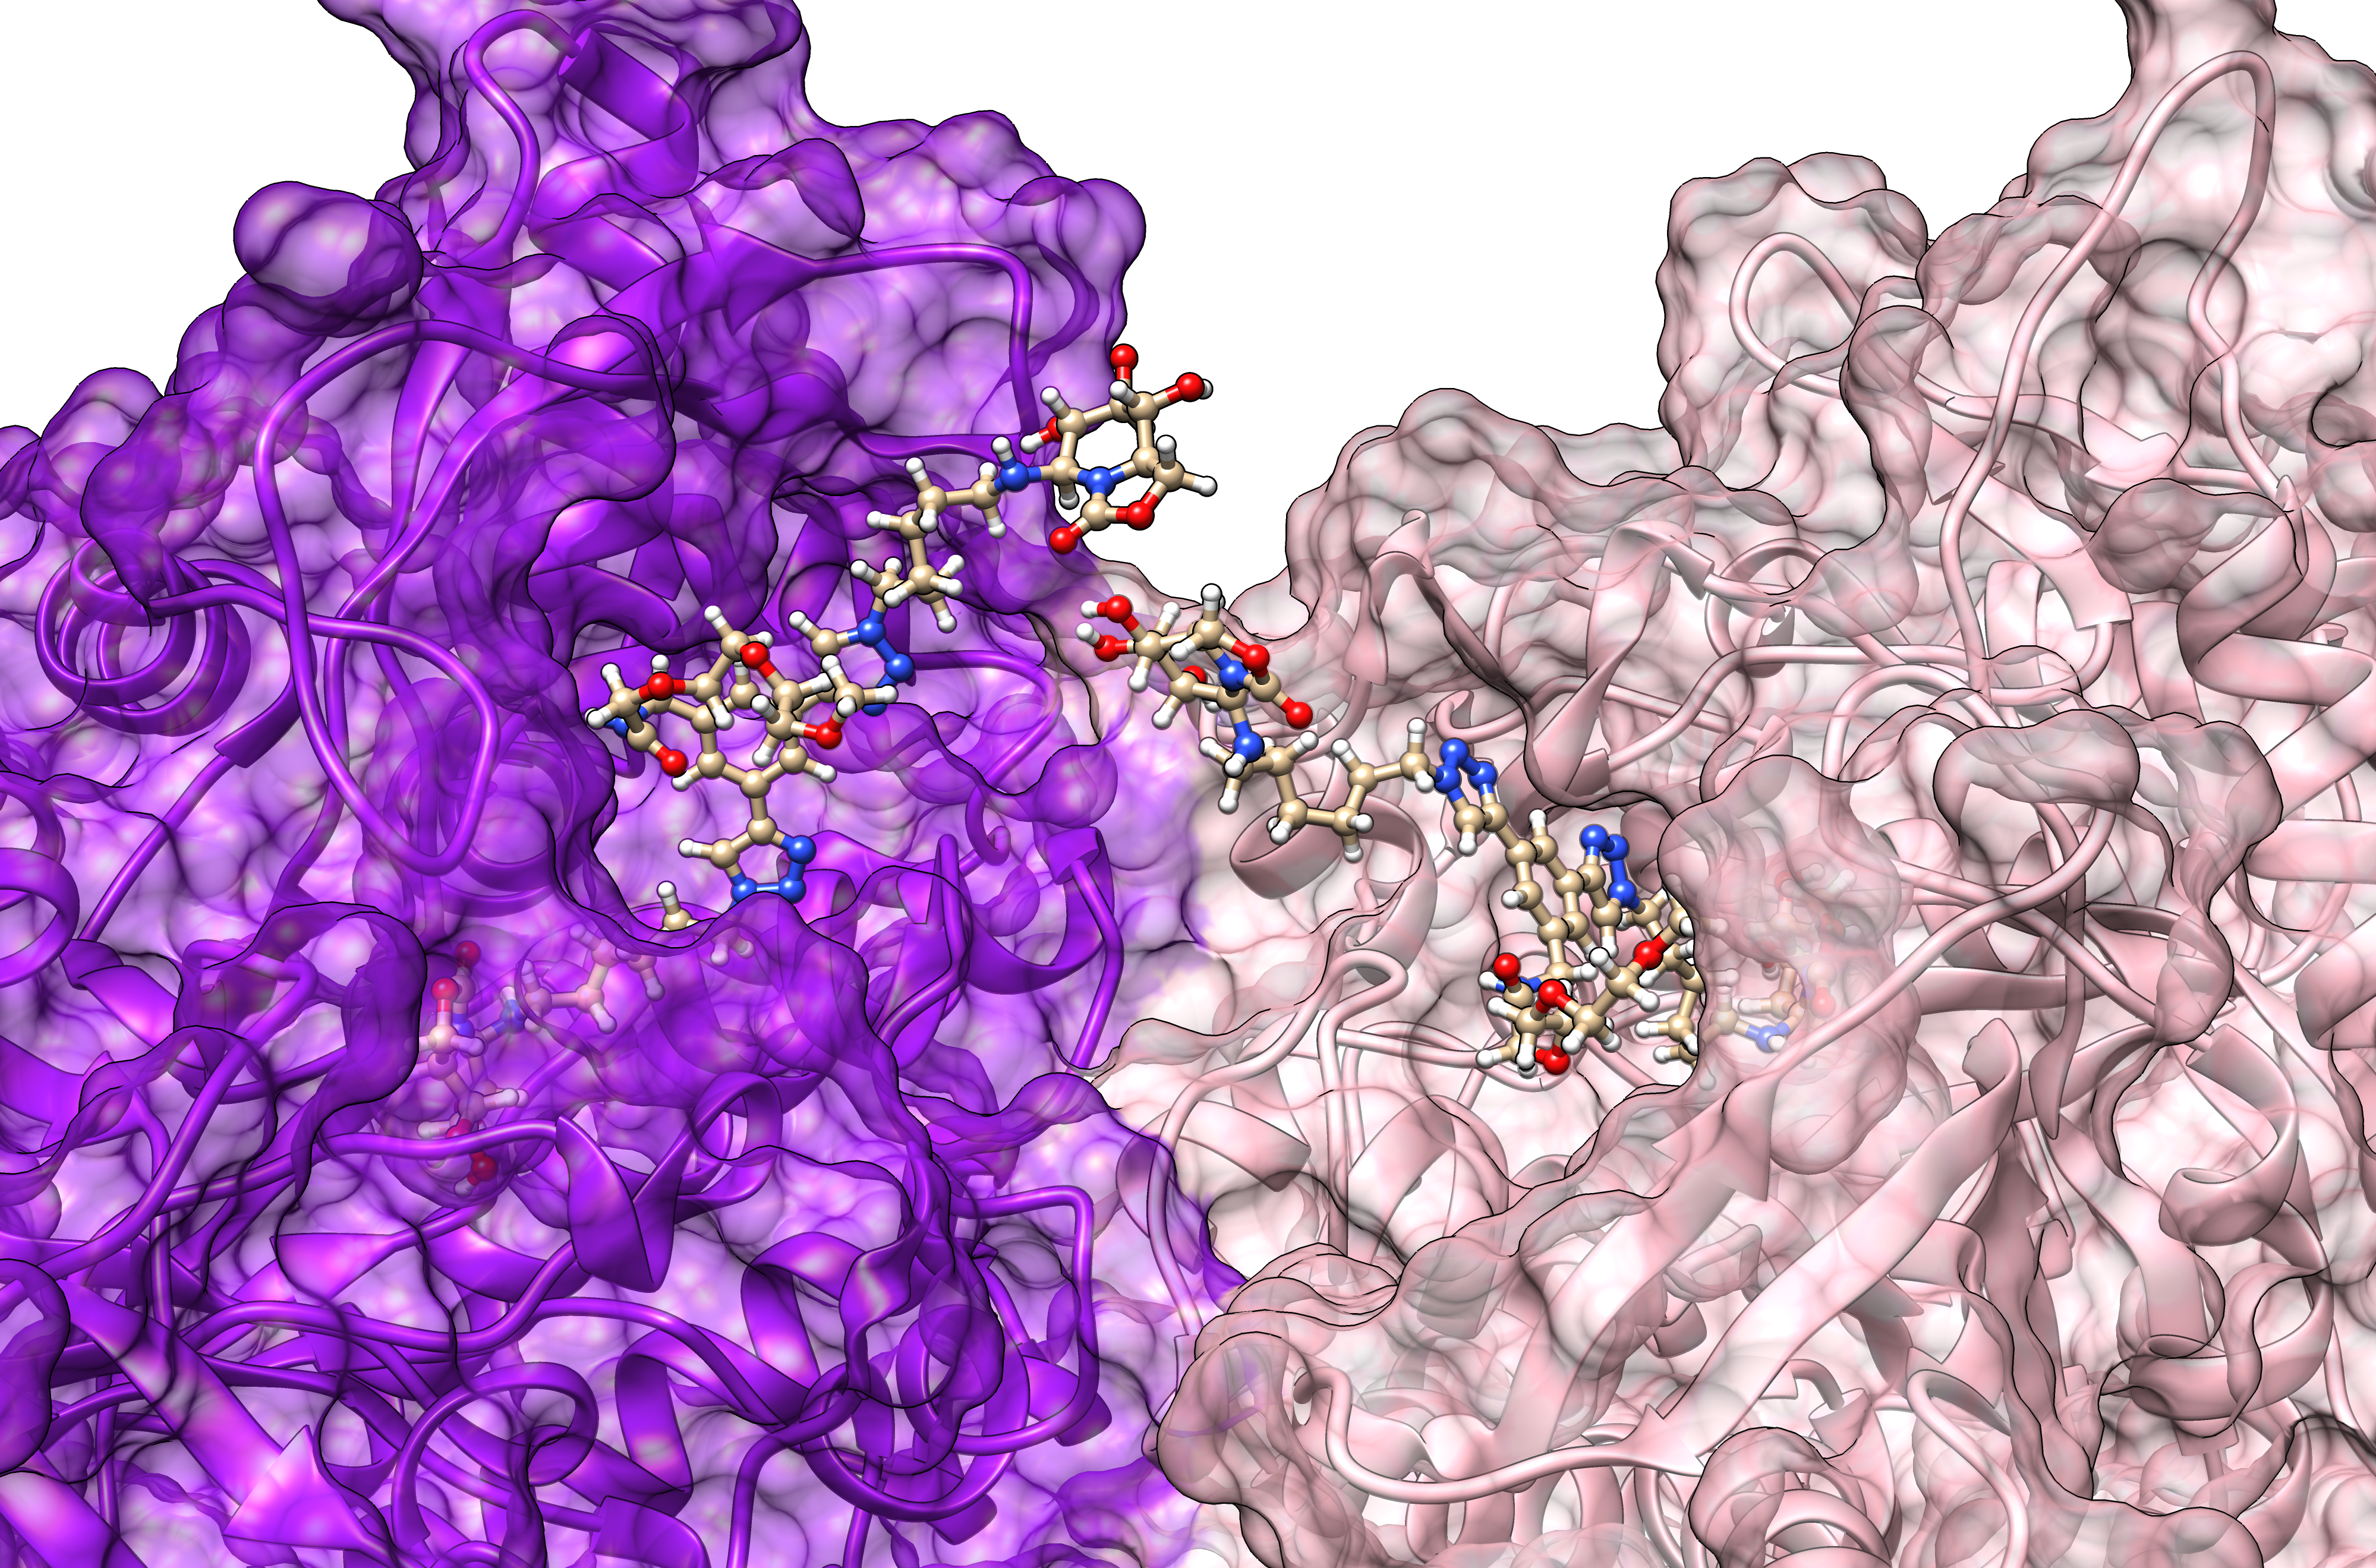
\includegraphics[width=\textwidth]{./figures/06/divalent-interface-meeting.png}
	\end{Center}
	\caption[Dual di-ONJ interface meeting test]{Two divalent ONJ models were anchored to their respective binding sites, and their free-torsion bonds were explored to find a pose were the two free iminosugar ends could interact at the interface via a H-bond.}
	\label{fig:divalent-interface}
\end{figure}


The analysis showed that this interaction is structurally feasible, which was further confirmed by an explicitly solvated, full-atom molecular dynamics trajectory: the interaction remained stable for more than 100 nanoseconds. Simulating this system (100,000+ atoms) for such a long period can take months with ordinary CPUs, but thanks to the GPU acceleration implemented in OpenMM and OMMProtocol (see \autoref[section]{section:ommprotocol}), these trajectories could be obtained within a week.\footnote{An equivalent protocol in the commercial, GPU-accelerated version of Amber installed in our facilities would have taken two weeks.}

While the computational model offers an answer to whether this structure is possible of not, this specific protocol cannot answer whether this interaction is favored. To assess that possibility, broader sampling would be needed (like metadynamics), which demanded more computational time than the available within the submission deadline. Additionally, there is no experimental information to support this hypothetic interaction: the stoichiometry suggested leans towards 1:1, and not 2:1.

\subsubsection{Does the rotaxane compound fit? Can it occupy both sites? How?}
% \addcontentsline{toc}{subsubsection}{Does the rotaxane compound fit? Can it occupy both sites? How?}
The pillar[5]ene variants exhibit a slightly worse $K_{i}$ but still comparable to the di-ONJ compound, so one would expect a similar interaction profile. The divalent ligand has been shown that it cannot reach both sites of a dimer, suggesting that its inhibition mechanism might be based on a sliding motion between the binding sites. However, the divalent ligand only represents half of the H-shaped component of the rotaxane compound. This has two conflicting consequences: (1) the H-shaped component is larger and could use the iminosugars of opposed axels to reach both binding sites, and (2) the volume of the crown component might work against this interaction through steric impediment. This raises two possibilities:

\begin{enumerate}
	\item The rotaxane interacts with the protein via iminosugars on the \textbf{same} axel.
	\begin{enumerate}
		\item This interaction strategy does not offer any advantage over the divalent binding (its iminosugar-iminosugar range distance is the same).
		\item The steric impediments of the crown component are easier to solve, since rest of the structure would remain facing the outside part of the structure.
	\end{enumerate}
	\item The rotaxane interacts with the protein via iminosugars on \textbf{different} axels.
	\begin{enumerate}
		\item The iminosugar-iminosugar range distance is far greater and could enable accessing both sites simultaneously.
		\item The steric impediments of the crown are far greater, since the structure would be now in a less ideal orientation.
	\end{enumerate}
\end{enumerate}

To assess both possibilities, the protein-rotaxane structure was analysed with GaudiMM following the same recipe as the single divalent molecule docking in \autoref[section]{section:di-ONJ-stretch}: one iminosugar was fixed in one binding site and the second one was instructed to get close to the second binding site with a distance minimization objective by exploring the free torsion of rotatable bonds. Steric clashes were minimized through a Contacts objective. See table \ref{table:recipe-rotaxane} for more details.

In the binding mode A (same axel), the structure did not reach the second binding site, as expected; not even tolerating severe clashes. In binding mode B (different axels), the H-shaped component could reach both sites comfortably. There were clashes, but not as bad as expected: they were mainly due to internal clashes of the rotaxane. Given the unusually high number of freely rotatable bonds (176 in this case), more iterations would have been needed to optimize them out. However, that was not necessary, since the purpose of these GaudiMM calculations was to obtain a \textit{good enough} structure to use as the starting point of the next step in the multiscale protocol.


\begin{table}[hbtp]
	\caption[Pillar-5-ene recipe]{Recipe used in the evaluation of the pillar[5]ene ligand. The ligand wass positioned in such a way that one of the terminal iminosugars matched the crystallographic structure of the ligand in one of the monomers of the original 2WBG protein structure.}
	\label{table:recipe-rotaxane}
	\footnotesize
	\newcolumntype{R}{>{\hsize=.25\hsize\raggedleft\arraybackslash}X}%
	\newcolumntype{L}{>{\hsize=.75\hsize\raggedright\arraybackslash}X}%
	\newcommand{\tableheading}[1]{\multicolumn{2}{c}{\textsc{#1}}}
	\begin{tabularx}{\textwidth}{RL}
		\toprule
		%row no:1
		\tableheading{Genes}\\
		\toprule
		%row no:2
		\texttt{Molecule} & Load the protein model obtained after cleaning the PDB structure\cite{pdb:2wbg} (waters and ligands removed) \\
		\midrule
		%row no:3
		\texttt{Molecule} & Load the structure of the pillar[5]ene as obtained through a preliminary 3D model in ChemCraft \\
		\midrule
		\texttt{Torsion} & Explore the free rotations of the pillar[5]ene \\
		\toprule
		%row no:4
		\tableheading{Objectives}\\
		\toprule
		%row no:5
		\texttt{Contacts} & Minimize steric clashes \\
		\midrule
		%row no:6
		\texttt{Distance} & Bring one of the free iminosugar ends (depending on the case studied, from the same axel or from the one across) closer to the binding site in monomer B \\

		\bottomrule

	\end{tabularx}
\end{table}

Once parameterized with Antechamber,\cite{wang2001antechamber} two candidate structures of each binding mode were submitted to a molecular dynamics analysis with OMMProtocol. Both revealed stable bindings to their respective sites, with additional stabilization of the structure via internal cross-interactions.

The unsurprising results observed for binding mode A (same axel) agree with the experimental evidences. It exhibits the same binding profile as a single divalent molecule, compatible with the sliding mechanism, hence the comparable $K_{i}$ values. The slight difference might be due to the entropic stabilization of the crown-component via secondary binding sites.

Unfortunately, while the binding mode B (different axels) showed a promising interaction profile, there is no experimental evidence to back it up. If this binding mode was feasible, a higher $K_{i}$ should be observed, but that is not the case.

\subsection{Discussion \& Further work}
% \addcontentsline{toc}{subsection}{Discussion $\&$  Further work}
This joint study was an excellent opportunity to show how GaudiMM can be a valuable asset for both experimental and computational communities. The computational feedback has provided illustrative models on what can be happening at the molecular level and even proposed alternative explanations to be confirmed experimentally. This can be argued in three points.

First, GaudiMM can provide results directly applicable to the wet-lab. The different di-ONJ variants tested opened doors to synthesizing ligands of optimum length that would explain how the di-ONJ ligand exhibits that excellent inhibition power without incurring in additional costs. Doing this experimentally would have involved more steps of synthesis and tests, only to discard most of the candidate ligands. With this computational framework, this can be obtained within a day. Of course, this does not replace the experimental data; it just reflects that computational assessment can at least provide a way to save material and human resources.

Second, it allows to create new types of computational studies in a simpler, consistent way. Testing if the di-ONJ compound or the rotaxane can reach both binding sites of a dimeric protein would be normally done with a steered molecular dynamics simulation. However, parameterization would be needed first. For the rotaxane alone, this would take more than a day. The actual simulation would take around a week. With GaudiMM, this can be obtained in hours. Then, if the results are positive, a MD simulation would be in order. However, if the results did not show anything promising, those expensive computational and time resources could be invested in testing a different hypothesis. In the same fashion, testing if two divalent ONJ ligands can interact at the interface would usually be studied with molecular docking, but there is no software suite that can perform a multi-ligand, restrained study like the one herein presented.

Third, even if the researchers prefer to go straight to the MD stage without confirming the feasibility of the hypothesis first, they would still need to build the initial structure. The researcher usually constructs those manually, with the aid of an interactive 3D viewer and related tools. This is normally doable with small ligands, but it starts getting disturbingly complex when bigger structures are involved. Setting up a rotaxane model suitable for MD assessment would have involved hours of finetuning and trial-and-error attempts. With GaudiMM, these can be obtained automatically when the correct recipe is used.

Of course, GaudiMM is not the answer to every question. It only helps guide the creation of new hypothesis at the initial steps of the brainstorming. For more accurate results, higher levels of theory must be applied through more advanced protocols. Even molecular dynamics might not be enough if quantitative magnitudes are demanded, such as binding energy or free energy. To obtain those, one would have to employ broad sampling methods like metadynamics or free energy perturbation, hybrid schemes like QM/MM, or even QM calculations of reduced cluster models. Those are out the scope of this dissertation and could not be performed within the available timeframe.

\section{Final conclusions}
% \addcontentsline{toc}{section}{Final conclusions}
Throughout this chapter, it has been shown that, while computational studies can be strictly theoretical, there is no point in denying that molecular modeling is a helpful tool for experimental works. \textit{In silico} can go hand in hand with \textit{in vitro}, and some research groups would argue that they must. It is common to see how experimental groups maintain strong alliances with theoretical groups. Fruitful joint efforts like this bring different points of view and ways of thinking to the discussion table, which can only enhance the brainstorming sessions, especially when counterintuitive phenomena like the aforementioned happen.


%!TEX root = ../dissertation.tex
\chapter{General conclusions}
\label{chap:07}

\Lettrine{In this dissertation} several computational tools have been presented and several applications have been benchmarked and showcased. Globally, the list of achievements could be summarized in six points:

% This approach useful for both molecular modelers and experimentalists.


\begin{enumerate}
	\item \textsc{GaudiMM} has been presented as a versatile molecular optimization framework with high modularity. Its uncoupled plurigenetic, multiobjective implementation provides researchers an unprecedented flexibility in molecular modeling. Instead of conforming to the requirements of a sequential multistep protocol, the same methods can work synergistically in the same modeling exercise. The concept of \textit{recipe} paves the way towards performing hypothesis-driven modeling as well as other simulations like dockings or restrained conformational exploration.

	\item \textsc{Tangram} is a collection of more than 15 tools for UCSF Chimera that will help in the generation of input files for 3\textsuperscript{rd} party software and diverse interactive structural analysis within a single graphical interface and user experience.

	\item \textsc{OMMProtocol} provides a user-friendly, single-file interface to the powerful, GPU-accelerated OpenMM molecular dynamics libraries. The communion of these tools have brought a 20-fold speed increase to the previously followed MD protocols in our group.

	\item \textsc{Garleek} has been designed to help in those QM/MM studies that require extended molecular mechanics force fields. By seamlessly interfacing Gaussian with modern MM suites, more accurate calculations can be obtained.

	\item \textsc{ESIgen} can save hours of manual text manipulation in computational chemistry. Its ability to automatically generate technical reports suitable for attachment as supporting information documents or internal communication with colleagues will be hopefully appreciated by this community. Computational chemists will also welcome \textsc{EasyMECP}, designed to facilitate the calculation of minimum energy crossing points (MECP) with Gaussian.

\end{enumerate}


These ongoing efforts have been the first steps towards developing a suite able to compete, feature-wise, with available commercial suites ---which can be particularly expensive in some cases--- at no cost for academics.

\subsection*{On GaudiMM}

In addition to reproducing and benchmarking known problems, this platform has been able to model orphan systems where currently available information is scarce. This is thanks to a versatile approach: creating optimization synergies between deliberate simplistic chemical and geometric descriptors. Some of the tasks that have benefitted from this idea are:

\begin{itemize}
	\item \textsc{Exotic docking prediction}. GaudiMM expands the possibilities of docking calculations beyond the traditional flexible protein-ligand dockings, enabling unconventional docking studies like competitive docking or multicovalent restraints (see \autoref[section]{section:proteinliganddocking} for a benchmark on standard protein-ligand docking and the take on more exotic cases).
	\item \textsc{Complex molecular design}. Predicting possible structures of partially characterized systems by performing hypothesis-driven modeling (see \autoref[section]{section:rotaxane} on multivalent enzyme inhibition). This includes designing complex ligands where only some experimental information is available, if any (see \autoref[section]{section:dibiotin-linker-length-optimization} for the optimization of a dibiotin ligand).
	\item \textsc{Finding metal binding sites in proteins}. Modeling organic systems where metal-residue interactions can be expressed with coordination geometries (see \autoref[section]{section:metal-applications} for this and other cases of coordination-driven folding).
\end{itemize}


Additionally, the conceptual separation of exploration and evaluation as implemented in GaudiMM gives a clear understanding of the different variables involved in an optimization process. This has proved to be a very valuable as a teaching tool in lower degrees of education. Students involved in GaudiMM development have contributed new modules even with a non-chemical background. Some highlights include a gene to navigate the chemical space or a coupled gene/objective pair to assess ligand binding pathways, detailed in \autoref[appendix]{chap:appendix-b}.


Of course, there is further work to do. GaudiMM's approach has a modestly steep learning curve and configuring an input file is mostly done by hand. A helper GUI for this task would be desirable and is something to consider in the short term, especially for specific applications (e.g. searching metal binding sites or optimizing the length of linkers).

Analysing results from a multi-objective optimization process could be a real tour de force because of the large number of possible solutions that needs to be filtered. , this hypothetical application-specific interfaces could also include a particular linearization of the multiobjective recipe. This way, the end-user should only look for a single score value. This would require parameterizing the weights of the linear sum by benchmarking big datasets. In this task, machine learning could be very helpful.

\section*{On Python}

Without Python and its great ecosystem (UCSF Chimera, the SciPy stack and the Omnia project have been particularly important) this dissertation would not have been possible. All the developments carried out during this Ph.D. are the consequences of its unique vision.

The \textit{de facto} Python installation already provides a library for high-level operations, freeing the developer from dealing with technical nuances. Beyond the official distribution, the catalog of ready-to-use packages is excellent, allowing to prototype projects in very little time just by importing the needed requirements. This is particularly true in scientific software, where it shines as the perfect glue language to stick different projects together.

Moreover, the emphasis on readibility and self-documented code contributes to maintaining good practices along the full development cycle, even when different people are involved. This is particularly important for long-lasting efforts in research and fruitful investment in research.

This Ph.D. hopefully illustrates how Python and its exceptional ecosystem offer molecular modelers with a versatile canvas for innovative science.

%!TEX root = ../dissertation.tex
\chapter*{Epilog}
\addcontentsline{toc}{chapter}{Epilog}
\label{chap:epilog}

During the development of new software, difficulties can arise anytime, for any reason. Dependencies, installation and distribution are inherent problems to the complex landscape of libraries, operating systems and hardware architectures. Solving them efficiently requires using developer-specific tools, usually disregarded by end-users. I began my Ph. D. studies as a user and ended up as some sort of developer, and to my surprise, my most popular project is not GaudiMM itself, but a tool created as a helper for its development: PyChimera. The need for interconnected software is patent, and a big part of this dissertation has been devoted to bringing new free alternatives to the table. The Tangram suite is only an attempt at providing molecular modeling tools accessible for beginner users that do not want to mess up with complex installations and input files: the workflow has been designed to be intuitive and consistent.

Still, most complex tasks would require some sort of scripting for an efficient solution. Programming skills are essential in all fields of science that can be enhanced by computational support. Two main properties can be identified: they can accelerate repetitive tasks, freeing time for other problems, and at the same time they enable new problem-solving strategies and can help plan studies in a different way. In other words, programming skills streamline creative thinking.

GaudiMM was a simple (but inefficient) for-loop doing conditional operations. It was the abstraction that followed that unlocked new possible workflows. New questions could be asked, new ideas could be devised. \textit{Is it possible to...?} started to have new endings.

Yet we are failing to convince students why coding is important. Most still prefer to go manually to \textit{make sure} results will be correct, and not a false positive product of a non-obvious bug. Is this due to the uninformative error messages, or does it go deeper in our educational system roots? Students are still taught memorization and mechanization, but that should not be the point in this era. Computers are much better at that than us, and will surpass us in other areas too. Solving problems is not copying algorithms and following instructions. It should be more about the reasons behind each of those steps. Designing algorithms, protocols, tools and frameworks: that should be the goal. Otherwise, the inability to write code will become the illiteracy of the XXI\textsuperscript{st} century.

\begin{appendices}
    \chapter*{Appendices}
    \makeatletter
        \if@twoside
            \fancyhf[reh]{\textit{Appendix \thechapter}}
            % insert blank page
            \pagestyle{empty}
            {
            \renewcommand{\thispagestyle}[1]{}
            \cleardoublepage
            }
            \newpage
            \thispagestyle{empty}
            \pagestyle{fancy}
        \fi
    \makeatother
    
    %!TEX root = ../dissertation.tex
\chapter{Perspectives for molecular modeling}
\label{chap:appendix-a}

% \addcontentsline{toc}{*}{The future of molecular modeling}
\Lettrine{In} an ideal future, there would be no need for multiscale protocols because accuracy compromises will not be needed in exchange for performance. However, to get there a large series of milestones must be conquered first. That path can only be pursued if there is a global interest.

\section*{The impact of molecular modeling}
\addcontentsline{toc}{section}{The impact of molecular modeling}
\label{molecular-modeling-impact}

Such a vast array of tools and resources can only be product of thousands of researchers, both in the public and private sector, and such devotion can only come if the field is attractive enough. Computational modeling is widely regarded as one of the fastest growing sectors in science, as perceived by researches and engineers themselves. According to a recent survey from the European FP7 project MULT-EU-SIM22, which measures the impact of general modeling in science and engineering, 75 $\%$  of researchers see a high impact of modeling and simulation in their fields, and 70 $\%$  foresee a strong growth of these methods, with an impact far beyond the one currently achieved.\cite{ENN2012} International institutions also believe in the trend and, in fact, there are several ongoing projects working on standardizing basic concepts such as the terminology to be employed.\cite{cen2017} The very existence of reports covering the topic\cite{Goldbeck2012,Goldbeck2016,goldbeck2017} also serves as support for this general idea.

More concrete examples of this perception include the aerospace industry, which uses computational chemistry to better understand the effect of high temperatures and combustion on the stability of the coating present in the materials employed, thus increasing flight safety. Additionally, nuclear reactors longevity is affected by the impact of neutrons on the walls, which result in atomic displacement evaluable with computational chemistry. Better determining the life expectancy of the reactor and can potentially save millions by preventing an early shutdown of the plant.\cite{UKeconomics} In pharma, measuring the heat of formation experimentally is 50 times more expensive than a comparable DFT study.\cite{maginn2009}

These anecdotical examples can be quantified by analyzing several metrics on each of the three levels of the knowledge transmission model:\cite{warry2006} (1) Authors, (2) Users, (3) Society. The authors of theories and models (1), usually belonging to the academia, publish their findings to scientific journals, which end up in software products that can be used by professional modelers (2), leading to process improvements. This directly benefits society with lower prices in value products (3).

The increased popularity in basic research can be measured by the number of published manuscripts mentioning the topic, as well as their specific proportion within the field and impact factor. Observing the increasing presence of techniques such as DFT or molecular dynamics is a good proxy to the trend, as evidenced in \citet{maginn2009}. An updated example can be seen in fig. \ref{fig:pubtrends}.


\begin{figure}[H]
	\includegraphics[width=\textwidth]{./figures/01/publication-trends_crop.pdf}
	\caption[Publication trends in molecular modeling]{Publication trends of manuscripts in molecular modeling in the title or abstract against all publications in chemistry related fields. Values are normalized against records in 2009. While publications in all chemistry failed exhibit a slower growth, articles in the field of molecular modeling (as represented with two popular methods, MD and DFT) have grown faster in the past decade. (Data obtained through dimensions.ai)}
	\label{fig:pubtrends}
\end{figure}


The direct application of methods is measurable by looking at the number of patents on the topic,\footnote{For example, at \url{http://www.wipo.int/patentscope} the return rate in the corresponding industries (between 3:1 and 10:1 in pharma, according to \citet{accelryswhitepaper},\cite{accelryswhitepaper} or the specific job postings demanding such experience.\footnote{Custom searches can be performed in websites such as \url{http://chemjobber.blogspot.com/}}, \url{http://www.linkedin.com}, \url{http://glassdoor.com} or \url{http://www.stackoverflow.com}}

In addition to the jobs themselves, which can be regarded as direct benefit for society, some other numbers could be thrown, such as the estimated contribution to the GDP by chemistry research (1.4$\%$  in UK as of 2010\cite{UKeconomics}), or the attributed spending on high performance computing by the modeling sectors, featuring bio-sciences, chemical engineering or computer-aided engineering as top contributors.\cite{hpc2020}

\begin{itemize}
	\item \href{https://eic.rsc.org/feature/the-rise-of-molecular-modeling/3007610.article}{https://eic.rsc.org/feature/the-rise-of-molecular-modeling/3007610.article}

	\item \href{http://www.sciencedirect.com/science/article/pii/S1359644608001529}{http://www.sciencedirect.com/science/article/pii/S1359644608001529}
\end{itemize}

\section*{What the next generation will bring to the table}
\addcontentsline{toc}{section}{What the next generation will bring to the table}

Published almost twenty years ago, the chapter "Vision 2020: Computational Needs of the Chemical Industry" in "Impact of Advances in Computing and Communications Technologies on Chemical Science and Technology: Report of a Workshop" cited five main computational challenges for the chemical industry: Predicting (1) biological activity and (2) toxicity of a chemical structure, and designing (3) catalysts, (4) chemical processes and (5) materials. This englobes two intertwined areas: prediction and design. For this to happen, the report points that intense research must be carried out in, amongst others, the potential functions of MM-based methods, long MD simulations for large ensembles (in the millisecond scale), quantum effects, solvent effects, solid state structure, multiscale protocols (atomistic, micro-, meso-, and macroscopic). Most of the challenges are accuracy or scale related, so huge efforts must be invested to reach errors within 0.1-0.2 kcal/mol in thermochemistry or to design universal and polarizable force fields, to cite two examples. This is not only a matter of scientific software development, but also responsibility of computer architecture, operating systems and networks. Since a single processor can only go so fast, tera-, peta- and exascales can only be achieved with parallel scaling, both within the processor itself (multicore architectures) and across symmetric machines (nodes within a cluster). For this to work reliably, operating systems and networks must be designed with fault tolerance in mind: if a core or node fails, the whole ensemble might fail as well.\cite{vision2020}

We are almost in 2020 now, and part of the predictions and demands have been fulfilled. Massively parallel architectures are now inevitably present and software has been slowly adapting to the new design paradigms. Any research group or company can get access to these resources thanks to the ubiquitous \textit{cloud}, which offer hardware solutions on demand. The so-called \textit{as a Service}  products (Software as a Service, Platform as a Service$ \ldots $ ) allow per-usage payments without having to worry about maintenance or resource constraints. If a given simulation needs more storage, memory or calculation speed, more nodes can be added to the ensemble with a click. Platforms such as Amazon’s AWS, Google’s Cloud or Microsoft’s Azure\footnote{\url{https://aws.amazon.com}, \url{https://cloud.google.com}, \url{https://azure.microsoft.com}, respectively} provide the raw infrastructure, which can be configured by the researchers or employees themselves, but is more commonly setup by specialized companies devoted to this newly found market niche.

What this report did not anticipate was the advent of GPGPU (General Purpose Graphical Processor Unit) computing: the advances in 3D acceleration and desktop graphics cards proved to be a massively parallel architecture that could exploited by software not related to games and visualization. Molecular Dynamics simulation have seen a drastic performance increase thanks to this new paradigm, implemented in major MD software (Amber, Charmm, Gromacs, NAMD, HTMD, AceMD, OpenMM$ \ldots $ ) and is now possible to simulate hundreds of nanoseconds a day with a sub-1000$\$$  personal desktop, thus getting closer to the millisecond-scale proposed that, while not routinely common, is starting to hit journals more often.\cite{shaw2008anton,lane2013} Quantum Mechanics could certainly benefit from GPU acceleration, but the offer is still reduced (BigDFT,\cite{genovese2011daubechies} TeraChem\cite{luehr2011dynamic}). The following years would certainly see a mainstream presence of GPU-implemented QM methods.

This would be in agreement with the 2017 Grimme’s computational chemistry wish list for the upcoming 25 years: (1) Development of robust and fast electronic structure methods with chemical accuracy for all conceivable chemical processes, all states (gas, liquid, solid), and all (even exotic) types of spectroscopies, (2) Seamless and automated multilevel modeling, including error estimates, (3) Routine treatments for many nuclear degrees of freedom and entropy, (4) Inclusion of solvation effects, (5) Prediction of molecular as well as macroscopic (bulk) properties, and (6) Automated approaches for finding new reactions. Warshel, in his 2014 Nobel Lecture, pointed to broader future directions, like using molecular modeling to fight drug resistance, grasp a deeper understanding of protein-protein interactions, truly rational enzyme design or developing molecular machines; for all of them, multiscale strategies will be necessary, he concluded.\cite{Warshel2014}

These predictions can be further extended with more specific wishes, like universal reactive force fields or cheap, large-scale QM methods, two trends that will inevitably close the gap between these traditionally divergent approaches. Faster architecture and software will possibly allow for more robust ab initio protein structure and folding studies,\cite{Lee2017} and cheminformatics tools like (3D)QSAR will also see advances, as proposed by \citet{Cherkasov2013} Also, thanks again to hardware advances originally intended for gaming, Virtual and Augmented Realities will become mainstream and that should also influence molecular modeling software, whose graphical interfaces, built around an interactive 3D viewer, will be certainly enriched. As a matter of fact, several suites already include preliminary support.\cite{chimerax} Together with mobile and web platforms, desktop software will surely evolve to new interface paradigms.

Finally, a very hyped topic lately is the incursion of machine learning and neural networks in scientific software. After gaining a huge popularity for successfully solving problems traditionally understood as "easy for humans but hard for computers"  (i.e. facial recognition, natural language interfaces, speech synthesis), it is now overflowing to fields like computational chemistry. Being such a hot topic, a lot of publications have arisen in the last years (see fig. \ref{fig:machinelearningtrends}). While some see these proposals as the definite solution to some chemistry problems like QSAR\cite{paliwal2015,Ma2015,schutt2016,goh2017,goh2017b,koutsoukas2017,mayr2016} or even DFT-trained electronic predictions,\cite{faber2017} a certain skepticism is also held by others\footnote{See \url{https://www.forbes.com/sites/brucebooth/2017/04/26/four-decades-of-hacking-biotech-and-yet-biology-still-consumes-everything/} and \url{https://www.biopharmatrend.com/post/49-research-in-ai-for-drug-discovery-is-overhyped-and-what-to-do-about-it/}, especially when it comes to the pharma industry and drug design.


\begin{figure}[H]
	\includegraphics[width=\textwidth]{./figures/01/publication-trends-ml_crop.pdf}
	\caption[Machine learning publication trends]{Number of publications containing \textit{machine learning}  in title or abstract, per year. Data is normalized against the values recorded for 2009. Physical and theoretical chemistry exhibit a steeper growth in the recent years.}
	\label{fig:machinelearningtrends}
\end{figure}


Besides traditional computers, nascent quantum computing will be able to implement some algorithms with unprecedented efficiency. Computational chemistry will be one of the most benefitted fields in that regard,\cite{lanyon2010towards,zeng2017first,reiher2017elucidating} as prototyped in several recent attempts.\cite{hellweg2017brick,kandala2017hardware,sim2018quantum,dumitrescu2018cloud}

% Papers:

% \begin{itemize}
% 	\item \href{https://www.acs.org/content/acs/en/careers/college-to-career/chemistry-careers/computational-chemistry.html}{https://www.acs.org/content/acs/en/careers/college-to-career/chemistry-careers/computational-chemistry.html}

% 	\item \href{http://onlinelibrary.wiley.com/doi/10.1002/anie.201709943/full}{http://onlinelibrary.wiley.com/doi/10.1002/anie.201709943/full}

% 	\item \href{https://www.sciencedirect.com/science/article/pii/S0166354215300152}{https://www.sciencedirect.com/science/article/pii/S0166354215300152}

% Reading:

% 	\item \href{https://hub.wiley.com/community/exchanges/discover/blog/2014/02/05/a-day-in-the-life-of-a-computational-chemist}{https://hub.wiley.com/community/exchanges/discover/blog/2014/02/05/a-day-in-the-life-of-a-computational-chemist}

% 	\item \href{http://sciencenordic.com/nanomedicines-future-will-build-quantum-chemistry}{http://sciencenordic.com/nanomedicines-future-will-build-quantum-chemistry}

% 	\item \href{https://medium.com/@ShaliniAnanda1/ai-and-the-future-of-computational-chemistry-220dc462e092}{https://medium.com/@ShaliniAnanda1/ai-and-the-future-of-computational-chemistry-220dc462e092}

% 	\item \href{https://mariobarbatti.wordpress.com/2013/12/15/is-there-a-fair-future-for-computational-theoretical-chemistry/}{https://mariobarbatti.wordpress.com/2013/12/15/is-there-a-fair-future-for-computational-theoretical-chemistry/}

% 	\item \href{https://www.researchgate.net/post/What\_is\_the\_future\_in\_computational\_Chemistry\_I\_really\_want\_to\_know\_because\_i\_am\_planing\_to\_do\_my\_PhD\_in\_the\_said\_field\_Ur\_suggestions\_wil\_hlp\_me}{https://www.researchgate.net/post/What\_is\_the\_future\_in\_computational\_Chemistry\_I\_really\_want\_to\_know\_because\_i\_am\_planing\_to\_do\_my\_PhD\_in\_the\_said\_field\_Ur\_suggestions\_wil\_hlp\_me}

% 	\item \href{https://www.reddit.com/r/chemistry/comments/5v8glr/what\_does\_the\_future\_of\_computational\_chemistry/}{https://www.reddit.com/r/chemistry/comments/5v8glr/what\_does\_the\_future\_of\_computational\_chemistry/}

% 	\item \href{https://www.quora.com/What-is-the-future-of-computational-chemistry}{https://www.quora.com/What-is-the-future-of-computational-chemistry}

% 	\item \href{https://news.ycombinator.com/item?id=12783673}{https://news.ycombinator.com/item?id=12783673}

% 	\item \href{http://blog.rguha.net/?p=1703}{http://blog.rguha.net/?p=1703}
% \end{itemize}

    \chapter{Undergoing developments in GaudiMM}
\label{chap:appendix-b}
% \addcontentsline{toc}{section}{GaudiMM as an educational tool: undergoing developments}


\section{Navigating the chemical space}
% \addcontentsline{toc}{section}{Navigating the chemical space}
GaudiMM already allowed to navigate the chemical space via the dynamic building capabilities of the Molecule gene, but it presented two limitations: (1) it is restricted to the provided fragments library, and (2) it only allows to construct linear concatenations of those fragments (i.e. no ramifications or rings).

A new approach based on graph theory and pharmacophore matching is being developed in our group as part of the Ph.D. thesis of J. E. Sánchez-Aparicio. This method, which interprets molecules as non-directed graphs that can grow and shrink arbitrarily, does not require any preexisting libraries and naturally considers ramifications. It has been successfully applied to propose designs of small molecule inhibitors for \textit{K. pulmoniae} NDM-1 $ \beta $ -lactamase.

\section{Finding ligand binding pathways}
% \addcontentsline{toc}{section}{Finding ligand binding pathways}
Docking studies provides insight on how a small molecule can interact with a bigger host molecule by assessing feasible binding poses. However, those are just static snapshots of a dynamic behavior. To study how the ligand reaches its binding sites, long molecular dynamics runs with steering restraints are needed and do not always guarantee a successful ligand pathway.

An alternative approach was considered for one of the MSc dissertations supervised during this Ph.D. The protein space was flooded with small probes placed in a tight grid and queried for steric impediments, resulting in points with higher or lower pseudo-energy scores. Then, lower-energy points were traversed from the outer regions of the protein in hopes of finding a continuous path that reached the ligand binding site. To consider the ligand size, shape or volume, a second step was proposed. The calculated paths were segmented in 5Å pieces and each of the resulting pieces was then submitted to a docking simulation with reduced search radius. The resulting structures were low-energy conformations of the ligand along the proposed pathway. All these poses were finally concatenated together to emulate a smooth trajectory ideal for depiction purposes.

This proof of concept proves how the versatility present in GaudiMM can be used as part of bigger protocols, and is being reimplemented as a gene able to guide the exploration of docking studies along feasible pathways in the Ph.D. studies of J. E. Sánchez-Aparicio.

    \subsection{Living with metal ions in macromolecules}
% \addcontentsline{toc}{subsection}{Living with metal ions in macromolecules}
One of the most exciting areas of molecular modeling sits at the frontier between organometallics and biochemistry, two fields that have been studied separately in computational chemistry for decades now. Globally, chemists exploit their features differently and, as such, present different computational challenges. Traditionally, organometallic systems feature a reduced number of atoms and accommodate transition metal centers within their structure, whose exotic electronic behavior can only be accurately computed with quantum chemistry approaches. Studies on biological problems such as the early work on folding of peptides and proteins had to face a larger number of atoms (hundreds or thousands) from the beginning, forcing the authors to use classical mechanics approaches to deal with the added dimensionality after realizing that the electronics of the system were not very important in that process.

However, metals do take part in biological processes as mainstream as oxygen transportation and muscle contraction. As such, the existence of metalloproteins cannot be neglected by the modeling community, who should bring these two areas together in a more seamless experience. Given the diverging efforts accumulated for decades, the gap is not easily overcome, but some solutions exist. Depending on the properties to study, one can resort to different approaches, as detailed below.

\subsubsection{Quantum Mechanics}
% \addcontentsline{toc}{subsubsection}{Quantum Mechanics}
Since quantum mechanics deal explicitly with the electronic shells of atoms, the immense diversity of electronic configurations of metal ions does not represent a problem. If such, the only challenge this might present is choosing the adequate functionals, basis sets or starting-point structures.

The challenge is more technical than scientific. While advances in DFT theories and hardware architectures allow us to deal with up to 500-atom systems in feasible timescales, this is still far from the number of atoms usually present in protein structures. For this, hybrid QM/MM studies are more adequate: the QM layer is responsible for dealing with the metal and its surroundings (at least, the first coordination sphere), while the, comparatively cheap, MM layer governs the rest of the structure. Even with this approach, time-dependent schemes still represent a huge computational effort, not to mention the difficulties in setting up the system adequately. One must still deal with layer boundaries effects or the parameterization needed for the MM calculations.

\subsubsection{Molecular Mechanics}
% \addcontentsline{toc}{subsubsection}{Molecular Mechanics}
Sometimes, QM is not necessary for a modeling study, since the metal might only play a structural role without exhibiting reactivity. In these cases, it is more interesting to gather an insight into the structural behavior of the system along time. Nowadays, for macromolecular systems, this is only feasible with molecular dynamics approaches, which require accurately parameterized force fields. Traditionally, force fields were developed to solve problems existing with proteins, nucleic acids and organic compounds,\cite{lifson1968consistent,allinger1973,momany1975energy} so historically transition metals have not been considered in force field development. Additionally, they present complexities not present in the reduced set of organic elements: several coordination geometries, different charge states, exotic polarizable behavior... As a result, dealing with metals in molecular mechanics is usually challenging. One must choose between (1) not considering them at all, (2) using a low-accuracy general-purpose force field, or (3) facing the tedious process of parameterization.

Ignoring or removing the metal ions can be acceptable in certain cases where they do not play a crucial role in the structure or dynamics of the system, but that is rarely the case. While general purpose force fields are numerous and heavily used, they mostly target organic compounds (such as CGenFF,\cite{Vanommeslaeghe2009} GAFF,\cite{Wang2004} Tripos 5.2 force field\cite{clark1989}). Only some include parameters for metal ions: UFF (for Universal Force Field,\cite{rappe1992} MMFF\cite{halgren1996}) covers the full periodic table, but Dreiding\cite{Mayo1990} only contains parameters for Na, Ca, Zn and Fe. While useful for organic chemistry, they are not as used in simulations including biological systems $ \{ $ $ \} $ , since they tend to rely on the Lennard-Jones based ‘nonbonded model’ $ \{ $ $ \} $ .

A feasible alternative for bio-containing systems is the so-called ‘bonded model’, which treats metal ion interactions with both bonded and non-bonded parameters; i. e., the metal is assumed to bond to some residues. Some of the protein-oriented force fields like AMBER\cite{amber} or CHARMM\cite{brooks1983} distribute force field extensions for some of the most common metal ions in proteins, such as hemo-coordinated iron, but mainly as examples on how custom parameters can be added in the software. These types of force field extensions are only valid for the context where the parameters were obtained; i. e., the iron parameters for the heme groups will not reproduce the behavior of iron in other organic contexts such as ferrocenes. While the file format is easily understood, the values of the parameters are not easy to obtain: one has to resort to experimental data or \textit{ab initio} calculations to get adequate constants for bonded (distances, angles, dihedrals) and nonbonded (electrostatic, Van der Waals) interactions. While an expert user can decide to obtain those values manually, the process is not trivial and some protocols and tools have appeared to assis. They are mostly based on the Seminario’s method and his FUERZA software,\cite{Seminario1996} such as MCPB, MCPB.py,\cite{li2016} VFDFT.\cite{zheng2016} Recently, alternative approaches based on machine and statistical learning, \cite{fracchia2017,li2017b} and non-Seminario strategies\cite{Burger2012, allen2017} have also appeared, but the principle remains the same: extract the information from \textit{ab initio} calculations. Given the complexity of the task, some specific force fields have arisen lately to provide parameters for certain metals:

\begin{itemize}
	\item \href{http://onlinelibrary.wiley.com/doi/10.1002/9780470125830.ch2/summary}{http://onlinelibrary.wiley.com/doi/10.1002/9780470125830.ch2/summary}

	\item \href{http://onlinelibrary.wiley.com/doi/10.1002/jcc.10171/full}{http://onlinelibrary.wiley.com/doi/10.1002/jcc.10171/full}

	\item \href{http://pubs.acs.org/doi/abs/10.1021/ic00068a012?journalCode=inocaj}{http://pubs.acs.org/doi/abs/10.1021/ic00068a012?journalCode=inocaj}

	\item \href{http://pubs.acs.org/doi/abs/10.1021/jp046244d}{http://pubs.acs.org/doi/abs/10.1021/jp046244d}

	\item \href{http://pubs.acs.org/doi/abs/10.1021/ja00001a001?journalCode=jacsat}{http://pubs.acs.org/doi/abs/10.1021/ja00001a001?journalCode=jacsat}

	\item \href{http://onlinelibrary.wiley.com/doi/10.1002/jcc.20634/full}{http://onlinelibrary.wiley.com/doi/10.1002/jcc.20634/full}

	\item \href{http://onlinelibrary.wiley.com/doi/10.1002/pssb.201248460/full}{http://onlinelibrary.wiley.com/doi/10.1002/pssb.201248460/full}

	\item \href{http://pubs.acs.org/doi/abs/10.1021/ct400952t}{http://pubs.acs.org/doi/abs/10.1021/ct400952t}
\end{itemize}

A radically different strategy consists of mimicking the interactions of the metal site with positively-charged pseudoatoms strategically placed at around 0.9 \AA from the metal nucleus following the vertices of the adequate coordination geometry. The Cationic Dummy Atom Model (CDAM) was introduced for Mn2+ ions by Aaqvist $\&$  Warshel in 1990\cite{aaqvist1990} and has been successfully implemented in further studies fore Zn, Mg, Ca, Fe, Co, Ni, Cu and more.\cite{duarte2014,lu2012proteins,Oelschlaeger_2007,Saxena_2013,Saxena_2014,Liao_2015,Pang_1999} Among its advantages, once parameterized the CDAM approach is context-independent, but it forces a fixed coordination number and geometry on the modeled metal site.

The application of polarizable force fields (Fluctuating Charge methods, ABEEM, Drude oscillators and rods, induced dipoles, AMOEBA, PFF) or more exotic models based on Angular Overlap and Valence Bond Theory are also promising approaches, but the additional calculations incur in a big performance penalty when compared to other strategies and still require additional parameterization. Further details on the topic can be found in the extensive review published by Li and Merz Jr. in 2017.\cite{li2017}

\subsubsection{Lower levels of theory}
% \addcontentsline{toc}{subsubsection}{Lower levels of theory}
If the study at hand does not require a molecular mechanics treatment, such as docking studies of virtual screening approaches, the parameterization problem is usually not present or, at least, not that complicated. Docking studies, which try to accommodate small compounds within macromolecules, have not considered metals for years, since they were originally designed to find drug-like, organic compounds suitable for the pharmaceutical industry. Fortunately, over time some of the most popular docking packages have included strategies to deal with metals,\cite{flexx} albeit sometimes they could only be part of the host (usually a protein), and not part of the probe (the ligand).\cite{verdonk2003improved} To overcome the problem, approaches inspired in the Cationic Dummy Atom Model implemented in MM studies have been designed (‘H-bond trick’): in this case, the dummy atoms are hydrogen atoms that behave as a hydrogen bond donor, a chemical feature commonly implemented in docking software.

Other approaches involve considering the metal problem as a geometric optimization problem, restraining their position with distances, angles and dihedrals measurements. This strategy is partially implemented in homology modeling software like MODELLER, \cite{Sali1993} and is one of the main features of the developments presented in this thesis (detailed in \autoref{chap:03}).

In cheminformatics, explicit consideration of atoms is not as important and strategies like the pharmacophoric studies only have to consider metals as a custom type of interaction hotspot.\cite{johns2009,kawasuji2012,carcelli2014,yang2016} In QSAR, a catalogue of metal empirical properties is enough to build the dataset.\cite{walker2012fundamental}


    %!TEX root = ../dissertation.tex

\chapter{Tangram extensions for analysis}
\label{appendix:more-tangram}

\section{Interaction analysis}
% \addcontentsline{toc}{subsection}{Interaction analysis}
\subsection{GaudiView}
% \addcontentsline{toc}{subsubsection}{GaudiView}
GaudiMM, described in \autoref{chap:04}, can generate tens of solutions including several ‘good-enough’ answers to the problem posed due to its multi-objective nature. Seeing them all in UCSF often meant waiting for all the files to load beforehand, even the ones you might not be interested in seeing. Additionally, hiding the current one to show the following one required more than one action. As a result, the GaudiView graphical interface was designed to overcome those difficulties by providing the following features:

\begin{itemize}
	\item Provide a tabular view of the results listing all the solutions in rows, and objective scores in columns. Rows can be sorted by one or more columns and filtered out by providing one or more cutoffs depending on the value of one column.

	\item Since the result index (\texttt{$\ast$ .gaudi-output} file) already contains the list of filenames and their scores, this is enough to display the initial table. Actual molecule objects are only loaded when its row is selected. This allows for fast browsing of only the requested solutions, without initial loading times.

	\item Every time one or more new rows are selected (with a mouse click or with keyboard arrows), the previously selected rows are hidden and the new ones are displayed.

	\item New selections can run any Chimera command specified in the command-line field below the table. This can be really useful to update the displayed residues around a ligand in protein-ligand docking, for example.

	\item Some clustering and rescoring utilities are also included for deeper analysis.
\end{itemize}

The architecture behind GaudiView does not depend on the initial data structure: a preprocessing step is performed to build the tabular data view, that ultimately servers molecules to the interactive canvas. Thanks to that, it’s easy to integrate other file formats that can benefit from this interface. Currently, GaudiView accepts solutions from GOLD and arbitrary lists of Mol2 files. In the future, more docking programs could be integrated, like AutoDock Vina or DOCK.

\subsection{NCIPlotGUI}
% \addcontentsline{toc}{subsubsection}{NCIPlotGUI}
NCIPlot is a widely used visualization method developed by Contreras-García et al\cite{nciplot} that uses non-covalent interaction indices derived from electronic density and its derivatives (\todo{CHECK XXX}) to help distinguish attractive interactions like Van der Waals, London dispersion forces or hydrogen bonds from repulsive ones like bad steric impediments. The original implementation is a FORTRAN program that requires specific input file with atomic coordinates and special keywords. While not difficult to write, it is still a small entry barrier.

With NCIPlotGUI, the input file is automatically generated from any opened molecule in UCSF Chimera and the calculation is run in the background. When the program is done, the results are loaded in the same UCSF Chimera instance and plotted as colored volume maps (see fig. \ref{fig:tangram-nciplot}). For large numbers of atoms, an alternative, 40-times faster CUDA implementation of the NCIPlot method\cite{nciplotcuda} is also supported and recommended for GPU-enabled computers.



\begin{figure}
	\begin{Center}
		\includegraphics[width=\textwidth]{./figures/05/tangram_nciplot.png}
		\caption[Tangram NCIPlotGUI]{Non-Covalent Interaction analysis of the partial structure of KUJLIK CSD structure $ \{ $ $ \} $ , with 70 atoms. The interface shows the input and configuration forms, as well as the Reduced Density Gradient (RDG) versus Density plot}
		\label{fig:tangram-nciplot}
	\end{Center}
\end{figure}

\subsection{PLIPGUI}
% \addcontentsline{toc}{subsubsection}{PLIPGUI}
Protein-Ligand Interaction Profiler (PLIP)\cite{salentin2015plip} is a Python utility to identify, list and represent non-covalent interactions between protein-ligand complexes. It depends on OpenBabel and VMD to work, but some UCSF Chimera integration is available. PLIPGUI is a Chimera extension that wraps PLIP in a graphical interface so all the tasks can be performed in a single program. The resulting will list all the identified interactions with a dynamic table that is updated depending on the binding site selected (if multiple are present). This can be coupled with docking studies to identify additional features implicitly described in the docking score.\footnote{For example, in GaudiView, the included \texttt{plip} command can be run for each solution, illustrating the possible cooperative tasks enabled with Tangram.}

\section{Structure analysis}
% \addcontentsline{toc}{subsection}{Structure analysis}

\subsection{3D-SNFG}
% \addcontentsline{toc}{subsubsection}{3D-SNFG}
Glycoproteins are proteins that feature oligosaccharidic cofactors and are actively researched for its involvement in recognition processes, metabolism and allergies. However, since they are essentially different variations or 6 or 5-member alkane rings with hydroxyl \todo{(or some other functional groups?)} substitutions, it is difficult to differentiate them visually when using classic 2D or 3D depictions. For that reason, the GLYCAM committee decided on a standardized 2D representation using colored geometric shapes called Symbol Nomenclature for Glycans (SNFG).\cite{snfg} A 3D implementation for VMD was developed by Thieker et al\cite{3dsnfg} in TCL language, and is the original 3D-SNFG project. This is a reimplementation of the same idea, but using Python and UCSF Chimera. It provides three alternative depictions, and the possibility to customize sizes and scales without modifying the source code (as it was expected in the original TCL implementation). The representation (see fig. \ref{fig:tangram-snfg}) can be switched on with the \texttt{snfg} command and switched off with \texttt{$ \sim $ snfg}.

\begin{figure}[t]
	\begin{Center}
		\includegraphics[width=\textwidth]{./figures/05/tangram_snfg.png}
	\end{Center}
	\cprotect\caption[Tangram 3D-SNFG]{3D-SNFG representation of glycoside exohydrolase from \textit{Hordeum vulgare}.\cite{3wlh}}
	\label{fig:tangram-snfg}
\end{figure}

\subsection{BondOrder}
% \addcontentsline{toc}{subsubsection}{BondOrder}
UCSF Chimera does not consider bond orders in the connectivity information it stores or represents. An approximate calculation is done during the parsing stage of molecule files to compute some internal atom types, but then that data is discarded. For some jobs, this information is important, though.

This extension provides a way to define an ‘order’ parameters manually in chimera.Bond objects, so it can be used by other extensions that could rely on it. For example, QMSetup could use it to write the connectivity matrix using proper bond orders instead of the default 1.0. When the order attribute is present, this extension enables alternative representations of the bond with additional decorations in the cylinder.

Additionally, the bond order information can be automatically computed with external libraries like RDKit, OpenBabel or AmberTools. The algorithms employed in that case are only applicable for small molecules though, so some work is needed when dealing with macromolecules. In those cases, template structures for common residues could be applied.

\subsection{OrbiTraj}
% \addcontentsline{toc}{subsubsection}{OrbiTraj}
OrbiTraj patches the Molecular Dynamics trajectory viewer already present in Chimera and adds support for loading volume files for each frame. For example, this can be useful for QM optimization calculations where orbitals data have been generated for each frame. By using the OrbiTraj patch, the XYZ trajectory can display the orbitals volumetric isosurfaces along the way, thus representing electronic density transfer. The package also ships some independent Python scripts that can be used to convert WFN files as provided by Gaussian to CUBE files compatible with UCSF Chimera loaders.


\subsection{PoPMuSiCGUI}
% \addcontentsline{toc}{subsubsection}{PoPMuSiCGUI}
PoPMuSiC\cite{dehouck2011popmusic} is a web service that can calculate potentially stabilizing mutation sites in protein and peptide structures. Users need to register an account before submitting their files, and once the results are computed, they can be download from the user web panel. The results are plain-text files that list the different mutations associated to each residue position and their calculated score. PoPMuSiCGUI can open these files along with the submitted protein structure and depict those scores in a dynamic, two-panel tabular view. Residues can be colored according to is ‘mutability’ score: positions that would stabilize under certain mutations will have a positive score and colored in a shade of green proportional to that score, while non-stabilizable positions would have a negative score and a red shade. Additionally, residue positions can be mutated to one of the proposed substitutions by using the Dunbrack's\cite{dunbrack1993backbone} and Dynameomics\cite{scouras2011dynameomics} rotamer libraries implemented in UCSF Chimera, which will have the changes immediately applied in the interactive 3D canvas.



\begin{figure} % FIXME!
	\begin{Center}
		\includegraphics[width=\textwidth]{./figures/05/tangram_popmusic.png}
	\end{Center}
	\cprotect\caption[Tangram PoPMuSiC GUI]{PoPMuSiC results for the trimeric Foldon of the T4 phagehead fibritin.\cite{1rfo} One of the monomers has been colored according to the stabilizing potential of a mutation in that position (red being destabilizing, green neutral, and blue stabilizing).}
	\label{fig:tangram-popmusic}
\end{figure}


\subsection{PropKaGUI}
% \addcontentsline{toc}{subsubsection}{PropKaGUI}
PropKa is a Python library developed by Jensen\cite{propka}  that calculates pKa values of protein residues under different environment pH values. PropKaGUI wraps this package to make it usable in UCSF Chimera with a simple graphical interface. After selecting the opened molecule to be analyzed and the pH value, the PropKa routines are run and the results are shown in a new dialog listing the calculated pKa value for each residue. \todo{Adequate hydrogens can be added in situ by taking that information into account.}

\subsection{SubAlign}
% \addcontentsline{toc}{subsubsection}{SubAlign}
UCSF Chimera provides several utilities for molecular superposition. The ‘matchmaker’ command allows to efficiently superpose protein structures using sequence alignment and homology score matrices as guiding criteria. For non-protein structures, the simple ‘match’ command is able to obtain the optimal superposition of two molecules, but only if atom pairs correspondences are manually provided. Several algorithms exist to identify the best atoms correspondences automatically,\cite{cho2006flame,girones2001tgsa} but none of them are implemented in Chimera. The SubAlign extension provides a command (no graphical interface currently) to superpose small molecules by applying several alignment protocols implemented in RDKit.\cite{rdkit} The root-mean-square deviation (RMSD) of the superposed molecules is also provided as a result of the alignment, so it can be used for that kind of analysis as well. If more than two molecules are provided, all of them are aligned against the first, and the average RMSD is reported. In the future, more algorithms can be implemented, with a particular focus on those coming from the Computer Vision field, where Point Set Registration problems are common.

\end{appendices}

% the back matter
\makeatletter
    \if@twoside
        \fancyhf[loh]{}%
        \fancyhf[reh]{}
    \fi
\makeatother
\backmatter

\end{document}
